\documentclass[11pt]{article}

    \usepackage[breakable]{tcolorbox}
    \usepackage{parskip} % Stop auto-indenting (to mimic markdown behaviour)
    

    % Basic figure setup, for now with no caption control since it's done
    % automatically by Pandoc (which extracts ![](path) syntax from Markdown).
    \usepackage{graphicx}
    % Keep aspect ratio if custom image width or height is specified
    \setkeys{Gin}{keepaspectratio}
    % Maintain compatibility with old templates. Remove in nbconvert 6.0
    \let\Oldincludegraphics\includegraphics
    % Ensure that by default, figures have no caption (until we provide a
    % proper Figure object with a Caption API and a way to capture that
    % in the conversion process - todo).
    \usepackage{caption}
    \DeclareCaptionFormat{nocaption}{}
    \captionsetup{format=nocaption,aboveskip=0pt,belowskip=0pt}

    \usepackage{float}
    \floatplacement{figure}{H} % forces figures to be placed at the correct location
    \usepackage{xcolor} % Allow colors to be defined
    \usepackage{enumerate} % Needed for markdown enumerations to work
    \usepackage{geometry} % Used to adjust the document margins
    \usepackage{amsmath} % Equations
    \usepackage{amssymb} % Equations
    \usepackage{textcomp} % defines textquotesingle
    % Hack from http://tex.stackexchange.com/a/47451/13684:
    \AtBeginDocument{%
        \def\PYZsq{\textquotesingle}% Upright quotes in Pygmentized code
    }
    \usepackage{upquote} % Upright quotes for verbatim code
    \usepackage{eurosym} % defines \euro

    \usepackage{iftex}
    \ifPDFTeX
        \usepackage[T1]{fontenc}
        \IfFileExists{alphabeta.sty}{
              \usepackage{alphabeta}
          }{
              \usepackage[mathletters]{ucs}
              \usepackage[utf8x]{inputenc}
          }
    \else
        \usepackage{fontspec}
        \usepackage{unicode-math}
    \fi

    \usepackage{fancyvrb} % verbatim replacement that allows latex
    \usepackage{grffile} % extends the file name processing of package graphics
                         % to support a larger range
    \makeatletter % fix for old versions of grffile with XeLaTeX
    
    % Packages for including animations and multimedia
    %\usepackage{animate}
    %\usepackage{media9}
    \usepackage{tabularx} % Usado para ajustar a largura da coluna em tabelas
\usepackage{adjustbox} % Para dimensionar o conteúdo (incluindo imagens)
    
    %\usepackage{multimedia}
    \@ifpackagelater{grffile}{2019/11/01}
    {
      % Do nothing on new versions
    }
    {
      \def\Gread@@xetex#1{%
        \IfFileExists{"\Gin@base".bb}%
        {\Gread@eps{\Gin@base.bb}}%
        {\Gread@@xetex@aux#1}%
      }
    }
    \makeatother
    \usepackage[Export]{adjustbox} % Used to constrain images to a maximum size
    \adjustboxset{max size={0.9\linewidth}{0.9\paperheight}}

    % The hyperref package gives us a pdf with properly built
    % internal navigation ('pdf bookmarks' for the table of contents,
    % internal cross-reference links, web links for URLs, etc.)
    \usepackage{hyperref}
    % The default LaTeX title has an obnoxious amount of whitespace. By default,
    % titling removes some of it. It also provides customization options.
    \usepackage{titling}
    \usepackage{longtable} % longtable support required by pandoc >1.10
    \usepackage{booktabs}  % table support for pandoc > 1.12.2
    \usepackage{array}     % table support for pandoc >= 2.11.3
    \usepackage{calc}      % table minipage width calculation for pandoc >= 2.11.1
    \usepackage[inline]{enumitem} % IRkernel/repr support (it uses the enumerate* environment)
    \usepackage[normalem]{ulem} % ulem is needed to support strikethroughs (\sout)
                                % normalem makes italics be italics, not underlines
    \usepackage{soul}      % strikethrough (\st) support for pandoc >= 3.0.0
    \usepackage{mathrsfs}
    

    
    % Colors for the hyperref package
    \definecolor{urlcolor}{rgb}{0,.145,.698}
    \definecolor{linkcolor}{rgb}{.71,0.21,0.01}
    \definecolor{citecolor}{rgb}{.12,.54,.11}

    % ANSI colors
    \definecolor{ansi-black}{HTML}{3E424D}
    \definecolor{ansi-black-intense}{HTML}{282C36}
    \definecolor{ansi-red}{HTML}{E75C58}
    \definecolor{ansi-red-intense}{HTML}{B22B31}
    \definecolor{ansi-green}{HTML}{00A250}
    \definecolor{ansi-green-intense}{HTML}{007427}
    \definecolor{ansi-yellow}{HTML}{DDB62B}
    \definecolor{ansi-yellow-intense}{HTML}{B27D12}
    \definecolor{ansi-blue}{HTML}{208FFB}
    \definecolor{ansi-blue-intense}{HTML}{0065CA}
    \definecolor{ansi-magenta}{HTML}{D160C4}
    \definecolor{ansi-magenta-intense}{HTML}{A03196}
    \definecolor{ansi-cyan}{HTML}{60C6C8}
    \definecolor{ansi-cyan-intense}{HTML}{258F8F}
    \definecolor{ansi-white}{HTML}{C5C1B4}
    \definecolor{ansi-white-intense}{HTML}{A1A6B2}
    \definecolor{ansi-default-inverse-fg}{HTML}{FFFFFF}
    \definecolor{ansi-default-inverse-bg}{HTML}{000000}

    % common color for the border for error outputs.
    \definecolor{outerrorbackground}{HTML}{FFDFDF}

    % commands and environments needed by pandoc snippets
    % extracted from the output of `pandoc -s`
    \providecommand{\tightlist}{%
      \setlength{\itemsep}{0pt}\setlength{\parskip}{0pt}}
    \DefineVerbatimEnvironment{Highlighting}{Verbatim}{commandchars=\\\{\}}
    % Add ',fontsize=\small' for more characters per line
    \newenvironment{Shaded}{}{}
    \newcommand{\KeywordTok}[1]{\textcolor[rgb]{0.00,0.44,0.13}{\textbf{{#1}}}}
    \newcommand{\DataTypeTok}[1]{\textcolor[rgb]{0.56,0.13,0.00}{{#1}}}
    \newcommand{\DecValTok}[1]{\textcolor[rgb]{0.25,0.63,0.44}{{#1}}}
    \newcommand{\BaseNTok}[1]{\textcolor[rgb]{0.25,0.63,0.44}{{#1}}}
    \newcommand{\FloatTok}[1]{\textcolor[rgb]{0.25,0.63,0.44}{{#1}}}
    \newcommand{\CharTok}[1]{\textcolor[rgb]{0.25,0.44,0.63}{{#1}}}
    \newcommand{\StringTok}[1]{\textcolor[rgb]{0.25,0.44,0.63}{{#1}}}
    \newcommand{\CommentTok}[1]{\textcolor[rgb]{0.38,0.63,0.69}{\textit{{#1}}}}
    \newcommand{\OtherTok}[1]{\textcolor[rgb]{0.00,0.44,0.13}{{#1}}}
    \newcommand{\AlertTok}[1]{\textcolor[rgb]{1.00,0.00,0.00}{\textbf{{#1}}}}
    \newcommand{\FunctionTok}[1]{\textcolor[rgb]{0.02,0.16,0.49}{{#1}}}
    \newcommand{\RegionMarkerTok}[1]{{#1}}
    \newcommand{\ErrorTok}[1]{\textcolor[rgb]{1.00,0.00,0.00}{\textbf{{#1}}}}
    \newcommand{\NormalTok}[1]{{#1}}

    % Additional commands for more recent versions of Pandoc
    \newcommand{\ConstantTok}[1]{\textcolor[rgb]{0.53,0.00,0.00}{{#1}}}
    \newcommand{\SpecialCharTok}[1]{\textcolor[rgb]{0.25,0.44,0.63}{{#1}}}
    \newcommand{\VerbatimStringTok}[1]{\textcolor[rgb]{0.25,0.44,0.63}{{#1}}}
    \newcommand{\SpecialStringTok}[1]{\textcolor[rgb]{0.73,0.40,0.53}{{#1}}}
    \newcommand{\ImportTok}[1]{{#1}}
    \newcommand{\DocumentationTok}[1]{\textcolor[rgb]{0.73,0.13,0.13}{\textit{{#1}}}}
    \newcommand{\AnnotationTok}[1]{\textcolor[rgb]{0.38,0.63,0.69}{\textbf{\textit{{#1}}}}}
    \newcommand{\CommentVarTok}[1]{\textcolor[rgb]{0.38,0.63,0.69}{\textbf{\textit{{#1}}}}}
    \newcommand{\VariableTok}[1]{\textcolor[rgb]{0.10,0.09,0.49}{{#1}}}
    \newcommand{\ControlFlowTok}[1]{\textcolor[rgb]{0.00,0.44,0.13}{\textbf{{#1}}}}
    \newcommand{\OperatorTok}[1]{\textcolor[rgb]{0.40,0.40,0.40}{{#1}}}
    \newcommand{\BuiltInTok}[1]{{#1}}
    \newcommand{\ExtensionTok}[1]{{#1}}
    \newcommand{\PreprocessorTok}[1]{\textcolor[rgb]{0.74,0.48,0.00}{{#1}}}
    \newcommand{\AttributeTok}[1]{\textcolor[rgb]{0.49,0.56,0.16}{{#1}}}
    \newcommand{\InformationTok}[1]{\textcolor[rgb]{0.38,0.63,0.69}{\textbf{\textit{{#1}}}}}
    \newcommand{\WarningTok}[1]{\textcolor[rgb]{0.38,0.63,0.69}{\textbf{\textit{{#1}}}}}
    \makeatletter
    \newsavebox\pandoc@box
    \newcommand*\pandocbounded[1]{%
      \sbox\pandoc@box{#1}%
      % scaling factors for width and height
      \Gscale@div\@tempa\textheight{\dimexpr\ht\pandoc@box+\dp\pandoc@box\relax}%
      \Gscale@div\@tempb\linewidth{\wd\pandoc@box}%
      % select the smaller of both
      \ifdim\@tempb\p@<\@tempa\p@
        \let\@tempa\@tempb
      \fi
      % scaling accordingly (\@tempa < 1)
      \ifdim\@tempa\p@<\p@
        \scalebox{\@tempa}{\usebox\pandoc@box}%
      % scaling not needed, use as it is
      \else
        \usebox{\pandoc@box}%
      \fi
    }
    \makeatother

    % Define a nice break command that doesn't care if a line doesn't already
    % exist.
    \def\br{\hspace*{\fill} \\* }
    % Math Jax compatibility definitions
    \def\gt{>}
    \def\lt{<}
    \let\Oldtex\TeX
    \let\Oldlatex\LaTeX
    \renewcommand{\TeX}{\textrm{\Oldtex}}
    \renewcommand{\LaTeX}{\textrm{\Oldlatex}}
    % Document parameters
    % Document title
    \title{Trabalho final Análise Numérica}
      \author{Luiz Fernando Bossa\thanks{l.f.bossa@posgrad.ufsc.br} \and Prof. Fermín S. V. Bazán}
    \date{Dezembro 2025}
    
    
    
    
    
    
% Pygments definitions
\makeatletter
\def\PY@reset{\let\PY@it=\relax \let\PY@bf=\relax%
    \let\PY@ul=\relax \let\PY@tc=\relax%
    \let\PY@bc=\relax \let\PY@ff=\relax}
\def\PY@tok#1{\csname PY@tok@#1\endcsname}
\def\PY@toks#1+{\ifx\relax#1\empty\else%
    \PY@tok{#1}\expandafter\PY@toks\fi}
\def\PY@do#1{\PY@bc{\PY@tc{\PY@ul{%
    \PY@it{\PY@bf{\PY@ff{#1}}}}}}}
\def\PY#1#2{\PY@reset\PY@toks#1+\relax+\PY@do{#2}}

\@namedef{PY@tok@w}{\def\PY@tc##1{\textcolor[rgb]{0.73,0.73,0.73}{##1}}}
\@namedef{PY@tok@c}{\let\PY@it=\textit\def\PY@tc##1{\textcolor[rgb]{0.24,0.48,0.48}{##1}}}
\@namedef{PY@tok@cp}{\def\PY@tc##1{\textcolor[rgb]{0.61,0.40,0.00}{##1}}}
\@namedef{PY@tok@k}{\let\PY@bf=\textbf\def\PY@tc##1{\textcolor[rgb]{0.00,0.50,0.00}{##1}}}
\@namedef{PY@tok@kp}{\def\PY@tc##1{\textcolor[rgb]{0.00,0.50,0.00}{##1}}}
\@namedef{PY@tok@kt}{\def\PY@tc##1{\textcolor[rgb]{0.69,0.00,0.25}{##1}}}
\@namedef{PY@tok@o}{\def\PY@tc##1{\textcolor[rgb]{0.40,0.40,0.40}{##1}}}
\@namedef{PY@tok@ow}{\let\PY@bf=\textbf\def\PY@tc##1{\textcolor[rgb]{0.67,0.13,1.00}{##1}}}
\@namedef{PY@tok@nb}{\def\PY@tc##1{\textcolor[rgb]{0.00,0.50,0.00}{##1}}}
\@namedef{PY@tok@nf}{\def\PY@tc##1{\textcolor[rgb]{0.00,0.00,1.00}{##1}}}
\@namedef{PY@tok@nc}{\let\PY@bf=\textbf\def\PY@tc##1{\textcolor[rgb]{0.00,0.00,1.00}{##1}}}
\@namedef{PY@tok@nn}{\let\PY@bf=\textbf\def\PY@tc##1{\textcolor[rgb]{0.00,0.00,1.00}{##1}}}
\@namedef{PY@tok@ne}{\let\PY@bf=\textbf\def\PY@tc##1{\textcolor[rgb]{0.80,0.25,0.22}{##1}}}
\@namedef{PY@tok@nv}{\def\PY@tc##1{\textcolor[rgb]{0.10,0.09,0.49}{##1}}}
\@namedef{PY@tok@no}{\def\PY@tc##1{\textcolor[rgb]{0.53,0.00,0.00}{##1}}}
\@namedef{PY@tok@nl}{\def\PY@tc##1{\textcolor[rgb]{0.46,0.46,0.00}{##1}}}
\@namedef{PY@tok@ni}{\let\PY@bf=\textbf\def\PY@tc##1{\textcolor[rgb]{0.44,0.44,0.44}{##1}}}
\@namedef{PY@tok@na}{\def\PY@tc##1{\textcolor[rgb]{0.41,0.47,0.13}{##1}}}
\@namedef{PY@tok@nt}{\let\PY@bf=\textbf\def\PY@tc##1{\textcolor[rgb]{0.00,0.50,0.00}{##1}}}
\@namedef{PY@tok@nd}{\def\PY@tc##1{\textcolor[rgb]{0.67,0.13,1.00}{##1}}}
\@namedef{PY@tok@s}{\def\PY@tc##1{\textcolor[rgb]{0.73,0.13,0.13}{##1}}}
\@namedef{PY@tok@sd}{\let\PY@it=\textit\def\PY@tc##1{\textcolor[rgb]{0.73,0.13,0.13}{##1}}}
\@namedef{PY@tok@si}{\let\PY@bf=\textbf\def\PY@tc##1{\textcolor[rgb]{0.64,0.35,0.47}{##1}}}
\@namedef{PY@tok@se}{\let\PY@bf=\textbf\def\PY@tc##1{\textcolor[rgb]{0.67,0.36,0.12}{##1}}}
\@namedef{PY@tok@sr}{\def\PY@tc##1{\textcolor[rgb]{0.64,0.35,0.47}{##1}}}
\@namedef{PY@tok@ss}{\def\PY@tc##1{\textcolor[rgb]{0.10,0.09,0.49}{##1}}}
\@namedef{PY@tok@sx}{\def\PY@tc##1{\textcolor[rgb]{0.00,0.50,0.00}{##1}}}
\@namedef{PY@tok@m}{\def\PY@tc##1{\textcolor[rgb]{0.40,0.40,0.40}{##1}}}
\@namedef{PY@tok@gh}{\let\PY@bf=\textbf\def\PY@tc##1{\textcolor[rgb]{0.00,0.00,0.50}{##1}}}
\@namedef{PY@tok@gu}{\let\PY@bf=\textbf\def\PY@tc##1{\textcolor[rgb]{0.50,0.00,0.50}{##1}}}
\@namedef{PY@tok@gd}{\def\PY@tc##1{\textcolor[rgb]{0.63,0.00,0.00}{##1}}}
\@namedef{PY@tok@gi}{\def\PY@tc##1{\textcolor[rgb]{0.00,0.52,0.00}{##1}}}
\@namedef{PY@tok@gr}{\def\PY@tc##1{\textcolor[rgb]{0.89,0.00,0.00}{##1}}}
\@namedef{PY@tok@ge}{\let\PY@it=\textit}
\@namedef{PY@tok@gs}{\let\PY@bf=\textbf}
\@namedef{PY@tok@ges}{\let\PY@bf=\textbf\let\PY@it=\textit}
\@namedef{PY@tok@gp}{\let\PY@bf=\textbf\def\PY@tc##1{\textcolor[rgb]{0.00,0.00,0.50}{##1}}}
\@namedef{PY@tok@go}{\def\PY@tc##1{\textcolor[rgb]{0.44,0.44,0.44}{##1}}}
\@namedef{PY@tok@gt}{\def\PY@tc##1{\textcolor[rgb]{0.00,0.27,0.87}{##1}}}
\@namedef{PY@tok@err}{\def\PY@bc##1{{\setlength{\fboxsep}{\string -\fboxrule}\fcolorbox[rgb]{1.00,0.00,0.00}{1,1,1}{\strut ##1}}}}
\@namedef{PY@tok@kc}{\let\PY@bf=\textbf\def\PY@tc##1{\textcolor[rgb]{0.00,0.50,0.00}{##1}}}
\@namedef{PY@tok@kd}{\let\PY@bf=\textbf\def\PY@tc##1{\textcolor[rgb]{0.00,0.50,0.00}{##1}}}
\@namedef{PY@tok@kn}{\let\PY@bf=\textbf\def\PY@tc##1{\textcolor[rgb]{0.00,0.50,0.00}{##1}}}
\@namedef{PY@tok@kr}{\let\PY@bf=\textbf\def\PY@tc##1{\textcolor[rgb]{0.00,0.50,0.00}{##1}}}
\@namedef{PY@tok@bp}{\def\PY@tc##1{\textcolor[rgb]{0.00,0.50,0.00}{##1}}}
\@namedef{PY@tok@fm}{\def\PY@tc##1{\textcolor[rgb]{0.00,0.00,1.00}{##1}}}
\@namedef{PY@tok@vc}{\def\PY@tc##1{\textcolor[rgb]{0.10,0.09,0.49}{##1}}}
\@namedef{PY@tok@vg}{\def\PY@tc##1{\textcolor[rgb]{0.10,0.09,0.49}{##1}}}
\@namedef{PY@tok@vi}{\def\PY@tc##1{\textcolor[rgb]{0.10,0.09,0.49}{##1}}}
\@namedef{PY@tok@vm}{\def\PY@tc##1{\textcolor[rgb]{0.10,0.09,0.49}{##1}}}
\@namedef{PY@tok@sa}{\def\PY@tc##1{\textcolor[rgb]{0.73,0.13,0.13}{##1}}}
\@namedef{PY@tok@sb}{\def\PY@tc##1{\textcolor[rgb]{0.73,0.13,0.13}{##1}}}
\@namedef{PY@tok@sc}{\def\PY@tc##1{\textcolor[rgb]{0.73,0.13,0.13}{##1}}}
\@namedef{PY@tok@dl}{\def\PY@tc##1{\textcolor[rgb]{0.73,0.13,0.13}{##1}}}
\@namedef{PY@tok@s2}{\def\PY@tc##1{\textcolor[rgb]{0.73,0.13,0.13}{##1}}}
\@namedef{PY@tok@sh}{\def\PY@tc##1{\textcolor[rgb]{0.73,0.13,0.13}{##1}}}
\@namedef{PY@tok@s1}{\def\PY@tc##1{\textcolor[rgb]{0.73,0.13,0.13}{##1}}}
\@namedef{PY@tok@mb}{\def\PY@tc##1{\textcolor[rgb]{0.40,0.40,0.40}{##1}}}
\@namedef{PY@tok@mf}{\def\PY@tc##1{\textcolor[rgb]{0.40,0.40,0.40}{##1}}}
\@namedef{PY@tok@mh}{\def\PY@tc##1{\textcolor[rgb]{0.40,0.40,0.40}{##1}}}
\@namedef{PY@tok@mi}{\def\PY@tc##1{\textcolor[rgb]{0.40,0.40,0.40}{##1}}}
\@namedef{PY@tok@il}{\def\PY@tc##1{\textcolor[rgb]{0.40,0.40,0.40}{##1}}}
\@namedef{PY@tok@mo}{\def\PY@tc##1{\textcolor[rgb]{0.40,0.40,0.40}{##1}}}
\@namedef{PY@tok@ch}{\let\PY@it=\textit\def\PY@tc##1{\textcolor[rgb]{0.24,0.48,0.48}{##1}}}
\@namedef{PY@tok@cm}{\let\PY@it=\textit\def\PY@tc##1{\textcolor[rgb]{0.24,0.48,0.48}{##1}}}
\@namedef{PY@tok@cpf}{\let\PY@it=\textit\def\PY@tc##1{\textcolor[rgb]{0.24,0.48,0.48}{##1}}}
\@namedef{PY@tok@c1}{\let\PY@it=\textit\def\PY@tc##1{\textcolor[rgb]{0.24,0.48,0.48}{##1}}}
\@namedef{PY@tok@cs}{\let\PY@it=\textit\def\PY@tc##1{\textcolor[rgb]{0.24,0.48,0.48}{##1}}}

\def\PYZbs{\char`\\}
\def\PYZus{\char`\_}
\def\PYZob{\char`\{}
\def\PYZcb{\char`\}}
\def\PYZca{\char`\^}
\def\PYZam{\char`\&}
\def\PYZlt{\char`\<}
\def\PYZgt{\char`\>}
\def\PYZsh{\char`\#}
\def\PYZpc{\char`\%}
\def\PYZdl{\char`\$}
\def\PYZhy{\char`\-}
\def\PYZsq{\char`\'}
\def\PYZdq{\char`\"}
\def\PYZti{\char`\~}
% for compatibility with earlier versions
\def\PYZat{@}
\def\PYZlb{[}
\def\PYZrb{]}
\makeatother


    % For linebreaks inside Verbatim environment from package fancyvrb.
    \makeatletter
        \newbox\Wrappedcontinuationbox
        \newbox\Wrappedvisiblespacebox
        \newcommand*\Wrappedvisiblespace {\textcolor{red}{\textvisiblespace}}
        \newcommand*\Wrappedcontinuationsymbol {\textcolor{red}{\llap{\tiny$\m@th\hookrightarrow$}}}
        \newcommand*\Wrappedcontinuationindent {3ex }
        \newcommand*\Wrappedafterbreak {\kern\Wrappedcontinuationindent\copy\Wrappedcontinuationbox}
        % Take advantage of the already applied Pygments mark-up to insert
        % potential linebreaks for TeX processing.
        %        {, <, #, %, $, ' and ": go to next line.
        %        _, }, ^, &, >, - and ~: stay at end of broken line.
        % Use of \textquotesingle for straight quote.
        \newcommand*\Wrappedbreaksatspecials {%
            \def\PYGZus{\discretionary{\char`\_}{\Wrappedafterbreak}{\char`\_}}%
            \def\PYGZob{\discretionary{}{\Wrappedafterbreak\char`\{}{\char`\{}}%
            \def\PYGZcb{\discretionary{\char`\}}{\Wrappedafterbreak}{\char`\}}}%
            \def\PYGZca{\discretionary{\char`\^}{\Wrappedafterbreak}{\char`\^}}%
            \def\PYGZam{\discretionary{\char`\&}{\Wrappedafterbreak}{\char`\&}}%
            \def\PYGZlt{\discretionary{}{\Wrappedafterbreak\char`\<}{\char`\<}}%
            \def\PYGZgt{\discretionary{\char`\>}{\Wrappedafterbreak}{\char`\>}}%
            \def\PYGZsh{\discretionary{}{\Wrappedafterbreak\char`\#}{\char`\#}}%
            \def\PYGZpc{\discretionary{}{\Wrappedafterbreak\char`\%}{\char`\%}}%
            \def\PYGZdl{\discretionary{}{\Wrappedafterbreak\char`\$}{\char`\$}}%
            \def\PYGZhy{\discretionary{\char`\-}{\Wrappedafterbreak}{\char`\-}}%
            \def\PYGZsq{\discretionary{}{\Wrappedafterbreak\textquotesingle}{\textquotesingle}}%
            \def\PYGZdq{\discretionary{}{\Wrappedafterbreak\char`\"}{\char`\"}}%
            \def\PYGZti{\discretionary{\char`\~}{\Wrappedafterbreak}{\char`\~}}%
        }
        % Some characters . , ; ? ! / are not pygmentized.
        % This macro makes them "active" and they will insert potential linebreaks
        \newcommand*\Wrappedbreaksatpunct {%
            \lccode`\~`\.\lowercase{\def~}{\discretionary{\hbox{\char`\.}}{\Wrappedafterbreak}{\hbox{\char`\.}}}%
            \lccode`\~`\,\lowercase{\def~}{\discretionary{\hbox{\char`\,}}{\Wrappedafterbreak}{\hbox{\char`\,}}}%
            \lccode`\~`\;\lowercase{\def~}{\discretionary{\hbox{\char`\;}}{\Wrappedafterbreak}{\hbox{\char`\;}}}%
            \lccode`\~`\:\lowercase{\def~}{\discretionary{\hbox{\char`\:}}{\Wrappedafterbreak}{\hbox{\char`\:}}}%
            \lccode`\~`\?\lowercase{\def~}{\discretionary{\hbox{\char`\?}}{\Wrappedafterbreak}{\hbox{\char`\?}}}%
            \lccode`\~`\!\lowercase{\def~}{\discretionary{\hbox{\char`\!}}{\Wrappedafterbreak}{\hbox{\char`\!}}}%
            \lccode`\~`\/\lowercase{\def~}{\discretionary{\hbox{\char`\/}}{\Wrappedafterbreak}{\hbox{\char`\/}}}%
            \catcode`\.\active
            \catcode`\,\active
            \catcode`\;\active
            \catcode`\:\active
            \catcode`\?\active
            \catcode`\!\active
            \catcode`\/\active
            \lccode`\~`\~
        }
    \makeatother

    \let\OriginalVerbatim=\Verbatim
    \makeatletter
    \renewcommand{\Verbatim}[1][1]{%
        %\parskip\z@skip
        \sbox\Wrappedcontinuationbox {\Wrappedcontinuationsymbol}%
        \sbox\Wrappedvisiblespacebox {\FV@SetupFont\Wrappedvisiblespace}%
        \def\FancyVerbFormatLine ##1{\hsize\linewidth
            \vtop{\raggedright\hyphenpenalty\z@\exhyphenpenalty\z@
                \doublehyphendemerits\z@\finalhyphendemerits\z@
                \strut ##1\strut}%
        }%
        % If the linebreak is at a space, the latter will be displayed as visible
        % space at end of first line, and a continuation symbol starts next line.
        % Stretch/shrink are however usually zero for typewriter font.
        \def\FV@Space {%
            \nobreak\hskip\z@ plus\fontdimen3\font minus\fontdimen4\font
            \discretionary{\copy\Wrappedvisiblespacebox}{\Wrappedafterbreak}
            {\kern\fontdimen2\font}%
        }%

        % Allow breaks at special characters using \PYG... macros.
        \Wrappedbreaksatspecials
        % Breaks at punctuation characters . , ; ? ! and / need catcode=\active
        \OriginalVerbatim[#1,codes*=\Wrappedbreaksatpunct]%
    }
    \makeatother

    % Exact colors from NB
    \definecolor{incolor}{HTML}{303F9F}
    \definecolor{outcolor}{HTML}{D84315}
    \definecolor{cellborder}{HTML}{CFCFCF}
    \definecolor{cellbackground}{HTML}{F7F7F7}

    % prompt
    \makeatletter
    \newcommand{\boxspacing}{\kern\kvtcb@left@rule\kern\kvtcb@boxsep}
    \makeatother
    \newcommand{\prompt}[4]{
        {\ttfamily\llap{{\color{#2}[#3]:\hspace{3pt}#4}}\vspace{-\baselineskip}}
    }
    

    
    % Prevent overflowing lines due to hard-to-break entities
    \sloppy
    % Setup hyperref package
    \hypersetup{
      breaklinks=true,  % so long urls are correctly broken across lines
      colorlinks=true,
      urlcolor=urlcolor,
      linkcolor=linkcolor,
      citecolor=citecolor,
      }
    % Slightly bigger margins than the latex defaults
    
    \geometry{verbose,tmargin=.5in,bmargin=1in,lmargin=0.7in,rmargin=0.5in}
    
    

\begin{document}
    
    \maketitle
    
    

    
    \begin{tcolorbox}[breakable, size=fbox, boxrule=1pt, pad at break*=1mm,colback=cellbackground, colframe=cellborder]
\prompt{In}{incolor}{ }{\boxspacing}
\begin{Verbatim}[commandchars=\\\{\}]
\PY{k}{using}\PY{+w}{ }\PY{n}{Plots}
\PY{k}{using}\PY{+w}{ }\PY{n}{LinearAlgebra}
\end{Verbatim}
\end{tcolorbox}

    \hypertarget{an-trabalho-final}{%
\section{Trabalho final Análise Numérica}}

    \hypertarget{considere-o-problema}{%
\subsection{ Considere o problema}\label{considere-o-problema}}

\[
\begin{cases}
u_{tt} - u_{xx} = 0 & x \in [0, \pi], t \geq 0 \\
u(x, 0) = \exp(-100(x - \pi/2)^2), \\
 u_t(x, 0) = 0 \\
u(0, t) = 0, \\
u_x(\pi, t) + \delta u_t(\pi, t) = 0,
\end{cases}
\]

Descreva métodos numéricos para resolver o problema de ondas 1D,
incluindo a análise de estabilidade dos esquemas discretos. Considere
\(\delta \in (0, 1]\). Apresente resultados numéricos para valores
distintos de \(t\) que ilustrem a evolução da solução.

    \hypertarget{preparando-a-edp}{%
\subsubsection{Preparando a EDP}\label{preparando-a-edp}}

    Vamos denotar por \[U_{i,j} = u(x_i,t_j)\]

e fazemos 
\begin{align}
x_i &= ih, & i=0,\ldots, N\\
t_j &= jk, & j=0,\ldots, T
\end{align}


    \begin{tcolorbox}[breakable, size=fbox, boxrule=1pt, pad at break*=1mm,colback=cellbackground, colframe=cellborder]
\prompt{In}{incolor}{ }{\boxspacing}
\begin{Verbatim}[commandchars=\\\{\}]
\PY{n}{f}\PY{p}{(}\PY{n}{x}\PY{p}{)}\PY{+w}{ }\PY{o}{=}\PY{+w}{ }\PY{n}{exp}\PY{p}{(}\PY{o}{\PYZhy{}}\PY{l+m+mi}{100}\PY{p}{(}\PY{n}{x}\PY{o}{\PYZhy{}}\PY{n+nb}{π}\PY{o}{/}\PY{l+m+mi}{2}\PY{p}{)}\PY{o}{\PYZca{}}\PY{l+m+mi}{2}\PY{p}{)}\PY{+w}{ }\PY{c}{\PYZsh{} curva inicial}
\end{Verbatim}
\end{tcolorbox}

            \begin{tcolorbox}[breakable, size=fbox, boxrule=.5pt, pad at break*=1mm, opacityfill=0]
\prompt{Out}{outcolor}{ }{\boxspacing}
\begin{Verbatim}[commandchars=\\\{\}]
f (generic function with 1 method)
\end{Verbatim}
\end{tcolorbox}
        
    \begin{tcolorbox}[breakable, size=fbox, boxrule=1pt, pad at break*=1mm,colback=cellbackground, colframe=cellborder]
\prompt{In}{incolor}{ }{\boxspacing}
\begin{Verbatim}[commandchars=\\\{\}]
\PY{c}{\PYZsh{} Vamos definir o domínio e plotar a curva inicial}
\PY{n}{N}\PY{+w}{ }\PY{o}{=}\PY{+w}{ }\PY{l+m+mi}{314}\PY{o}{*}\PY{l+m+mi}{2}
\PY{n}{h}\PY{+w}{ }\PY{o}{=}\PY{+w}{ }\PY{n+nb}{π}\PY{o}{/}\PY{p}{(}\PY{n}{N}\PY{o}{\PYZhy{}}\PY{l+m+mi}{1}\PY{p}{)}
\PY{n}{domain}\PY{+w}{ }\PY{o}{=}\PY{+w}{ }\PY{l+m+mi}{0}\PY{o}{:}\PY{n}{h}\PY{o}{:}\PY{n}{π}\PY{p}{;}
\PY{n}{h}
\end{Verbatim}
\end{tcolorbox}

            \begin{tcolorbox}[breakable, size=fbox, boxrule=.5pt, pad at break*=1mm, opacityfill=0]
\prompt{Out}{outcolor}{ }{\boxspacing}
\begin{Verbatim}[commandchars=\\\{\}]
0.005010514599026784
\end{Verbatim}
\end{tcolorbox}
        
    Vamos usar \(h\approx\) \texttt{5e-3}. Vejamos o perfil inicial da nossa
onda.

    \begin{tcolorbox}[breakable, size=fbox, boxrule=1pt, pad at break*=1mm,colback=cellbackground, colframe=cellborder]
\prompt{In}{incolor}{ }{\boxspacing}
\begin{Verbatim}[commandchars=\\\{\}]
\PY{n}{plot}\PY{p}{(}\PY{n}{domain}\PY{p}{,}\PY{+w}{ }\PY{n}{f}\PY{o}{.}\PY{p}{(}\PY{n}{domain}\PY{p}{)}\PY{p}{,}\PY{+w}{ }\PY{n}{label}\PY{o}{=}\PY{l+s}{\PYZdq{}}\PY{l+s}{u(x,0)}\PY{l+s}{\PYZdq{}}\PY{p}{)}
\end{Verbatim}
\end{tcolorbox}
 
            
\prompt{Out}{outcolor}{ }{}
    
    \begin{center}
    \adjustimage{max size={0.9\linewidth}{0.9\paperheight}}{Trabalho_final_AN_files/Trabalho_final_AN_8_0.pdf}
    \end{center}
    { \hspace*{\fill} \\}
    

    Vamos analisar suas condições de fronteira e como elas se traduzem em
relação aos \(U_{i,j}\).

\begin{itemize}
\tightlist
\item
  \$u\_t(x, 0) = 0 \$ nos diz que a velocidade inicial é zero.
\end{itemize}

Usando uma aproximação de primeira ordem, podemos escrever:

\[\frac{\partial}{\partial t} u(x,0) \approx \frac{U_{i,1}-U_{i,0}}{k} = 0 \implies U_{i,1} = U_{i,0} \]

\begin{itemize}
\item
  \$u(0, t) = 0 \$ \textbf{Condição de Diriclet}, nos diz que a onda
  está fixa em \((0,0)\), ou seja, \(U_{0,j}\equiv 0\)
\item
  \(u_x(\pi, t) + \delta u_t(\pi, t) = 0\) \textbf{Condição de
  Robin/Impedância}: nos diz que na ponta \(x=\pi\), parte da onda é
  refletida e parte é absorvida.
\end{itemize}

Usando uma aproximação de primeira ordem, podemos escrever
\[ \frac{U_{N,j}-U_{N-1,j}}{h} + \delta \frac{U_{N,j}-U_{N,j-1}}{k} = 0 \]

e fazendo \(\lambda = \tfrac{k}{h}\) podemos isolar \(U_{N,j}\)

\[U_{N,j} = \frac{\delta}{\lambda + \delta}U_{N,{j-1}} +\frac{\lambda}{\lambda + \delta} U_{N-1,j}\]

    \hypertarget{leapfrog}{%
\subsubsection{Leapfrog 🐸}\label{leapfrog}}

    Esquema da molécula do Leapfrog.

\begin{figure}
\centering
\caption{Esquema da molécula do Leapfrog}
\end{figure}

    Usando uma aproximação de segunda ordem para \(u_{xx}\) e \(u_{tt}\)
temos

\[
\frac{
  U_{i+i,j} - 2U_{i,j} + U_{i-1,j}
}{h^2} =
\frac{
  U_{i,j+1} - 2U_{i,j} + U_{i,j-1}
}{k^2}
\]

Isolando \(U_{i+1,j}\) temos

\[
U_{i,j+1} = 2U_{i,j} - U_{i,j-1} + \lambda^2\left(U_{i+1,j} - 2U_{i,j} + U_{i-1,j}\right), \qquad i=1,\ldots,N-1
\]

para \(i=0\) e \(i=N\), usamos as condições de fronteira descritas
anteriormente.

    \hypertarget{anuxe1lise-von-neumann-cfl}{%
\subsubsection{Análise von Neumann +
CFL}\label{anuxe1lise-von-neumann-cfl}}

Fazendo \[U_{i,j} = \xi^i e^{\mathcal{1} j \theta}\] com
\(\mathcal{1} = \sqrt{-1}\)

Para que o método seja estável, o erro não pode crescer com o tempo,
logo precisamos que \(|\xi| \le 1\)

Substituímos o ansatz na equação de diferenças
\[\xi^{i+1} e^{\mathcal{1} j \theta} = 2\xi^i e^{\mathcal{1} j \theta} - \xi^{i-1} e^{\mathcal{1} j \theta} + \lambda^2 \left[ \xi^i e^{\mathcal{1} (j+1) \theta} - 2\xi^i e^{\mathcal{1} j \theta} + \xi^i e^{\mathcal{1} (j-1) \theta} \right]\]

Dividimos toda a equação por \(\xi^{i-1} e^{\mathcal{1} j \theta}\)

\[\xi^2 = 2\xi - 1 + \lambda^2 \xi \left[ e^{\mathcal{1} \theta} - 2 + e^{-\mathcal{1} \theta} \right]\]

Usamos a identidade de Euler
\(e^{\mathcal{1} \theta} + e^{-\mathcal{1} \theta} = 2\cos\theta\)

\[\xi^2 - 2\xi + 1 = \lambda^2 \xi (2\cos\theta - 2)\]

Reorganizando o termo da direita usando a identidade trigonométrica
\(1 - \cos\theta = 2\sin^2\left(\frac{\theta}{2}\right)\)

\[2\cos\theta - 2 = -2(1 - \cos\theta) = -4\sin^2\left(\frac{\theta}{2}\right)\]

Substituindo de volta na equação

\[\xi^2 - 2\xi + 1 = \xi \left[ -4\lambda^2 \sin^2\left(\frac{\theta}{2}\right) \right]\]

Isso nos dá a equação característica quadrática

\[\xi^2 - 2\left[ 1 - 2\lambda^2 \sin^2\left(\frac{\theta}{2}\right) \right] \xi + 1 = 0\]

Para simplificar, vamos definir
\(A = 1 - 2\lambda^2 \sin^2(\frac{\theta}{2})\).

A equação fica \[\xi^2 - 2A\xi + 1 = 0\]

As raízes desta equação quadrática são:

\[\xi = \frac{2A \pm \sqrt{4A^2 - 4}}{2} = A \pm \sqrt{A^2 - 1}\]

    Para que o método seja estável (\(|\xi| \le 1\)), devemos analisar o
termo dentro da raiz (discriminante):

\begin{itemize}
\item
  Se \(A^2 > 1\) (Raízes Reais): As raízes são reais e distintas. Como o
  produto das raízes é \(c/a = 1\), se elas são reais e não são ambas 1
  ou -1, uma delas terá magnitude maior que 1. Isso resultaria em
  instabilidade.
\item
  Se \(A^2 \le 1\) (Raízes Complexas): O discriminante é negativo ou
  zero. As raízes são \(A \pm \mathcal{1}\sqrt{1-A^2}\). O módulo ao
  quadrado \[|\xi|^2 = A^2 + (\sqrt{1-A^2})^2 = A^2 + 1 - A^2 = 1\]Neste
  caso, \(|\xi| = 1\). Isso indica estabilidade neutra (o erro não
  cresce nem diminui, apenas oscila, o que é ideal para a equação da
  onda pois não introduz dissipação artificial).Portanto, a condição de
  estabilidade é
\end{itemize}

\[|A| \le 1\]

\[-1 \le 1 - 2\lambda^2 \sin^2\left(\frac{\theta}{2}\right) \le 1\]

\[0 \le 2 - 2\lambda^2 \sin^2\left(\frac{\theta}{2}\right) \le 2\]

\[0 \le 1 - \lambda^2 \sin^2\left(\frac{\theta}{2}\right) \le 1\]

    A desigualdade do lado direito é claramente satisfeita. A do lado
esquerdo precisa que
\[\lambda^2 \sin^2\left(\frac{\theta}{2}\right) \le 1\] o que significa
que para garantir a condição Courant-Friedrichs-Lewy devemos tomar
\(|\lambda|\le 1\).

    \hypertarget{resolvendo}{%
\subsubsection{Resolvendo}\label{resolvendo}}

    \begin{tcolorbox}[breakable, size=fbox, boxrule=1pt, pad at break*=1mm,colback=cellbackground, colframe=cellborder]
\prompt{In}{incolor}{ }{\boxspacing}
\begin{Verbatim}[commandchars=\\\{\}]
\PY{c}{\PYZsh{} LeapFrog}
\PY{n}{δ}\PY{+w}{ }\PY{o}{=}\PY{+w}{ }\PY{l+m+mf}{0.8}\PY{+w}{ }\PY{c}{\PYZsh{} parâmetro de absorção}
\PY{n}{λ}\PY{+w}{ }\PY{o}{=}\PY{+w}{ }\PY{l+m+mf}{0.9}\PY{+w}{ }\PY{c}{\PYZsh{}}
\PY{n}{k}\PY{+w}{ }\PY{o}{=}\PY{+w}{ }\PY{n}{λ}\PY{o}{*}\PY{n}{h}

\PY{n}{T}\PY{+w}{ }\PY{o}{=}\PY{+w}{ }\PY{l+m+mi}{5000}

\PY{n}{U0}\PY{+w}{ }\PY{o}{=}\PY{+w}{  }\PY{n}{f}\PY{o}{.}\PY{p}{(}\PY{n}{domain}\PY{p}{)}\PY{p}{;}
\PY{n}{U1}\PY{+w}{ }\PY{o}{=}\PY{+w}{ }\PY{n}{copy}\PY{p}{(}\PY{n}{U0}\PY{p}{)}\PY{p}{;}\PY{+w}{ }\PY{c}{\PYZsh{} U\PYZca{}1 = U\PYZca{}0}
\PY{n}{U}\PY{+w}{ }\PY{o}{=}\PY{+w}{ }\PY{p}{[}\PY{n}{U0}\PY{p}{,}\PY{+w}{ }\PY{n}{U1}\PY{p}{]}
\PY{n}{M}\PY{+w}{ }\PY{o}{=}\PY{+w}{ }\PY{n}{length}\PY{p}{(}\PY{n}{U0}\PY{p}{)}

\PY{k}{for}\PY{+w}{ }\PY{n}{j}\PY{o}{=}\PY{l+m+mi}{2}\PY{o}{:}\PY{n}{T}
\PY{+w}{  }\PY{n}{Ujp1}\PY{+w}{ }\PY{o}{=}\PY{+w}{ }\PY{n}{zeros}\PY{p}{(}\PY{n}{M}\PY{p}{)}\PY{+w}{ }\PY{c}{\PYZsh{} Ut[0] = 0 por condjção jnjcjal}
\PY{+w}{  }\PY{n}{Uj}\PY{+w}{ }\PY{o}{=}\PY{+w}{ }\PY{n}{U}\PY{p}{[}\PY{n}{j}\PY{p}{]}
\PY{+w}{  }\PY{n}{Ujm1}\PY{+w}{ }\PY{o}{=}\PY{+w}{ }\PY{n}{U}\PY{p}{[}\PY{n}{j}\PY{o}{\PYZhy{}}\PY{l+m+mi}{1}\PY{p}{]}
\PY{+w}{  }\PY{k}{for}\PY{+w}{ }\PY{n}{i}\PY{o}{=}\PY{l+m+mi}{2}\PY{o}{:}\PY{n}{M}\PY{o}{\PYZhy{}}\PY{l+m+mi}{1}\PY{+w}{  }\PY{c}{\PYZsh{} para os pontos jnterjores fazemos o esquema leapfrog}
\PY{+w}{    }\PY{n}{Ujp1}\PY{p}{[}\PY{n}{i}\PY{p}{]}\PY{+w}{ }\PY{o}{=}\PY{+w}{ }\PY{l+m+mi}{2}\PY{n}{Uj}\PY{p}{[}\PY{n}{i}\PY{p}{]}\PY{+w}{ }\PY{o}{\PYZhy{}}\PY{+w}{ }\PY{n}{Ujm1}\PY{p}{[}\PY{n}{i}\PY{p}{]}\PY{+w}{ }\PY{o}{+}\PY{+w}{ }\PY{n}{λ}\PY{o}{\PYZca{}}\PY{l+m+mi}{2}\PY{o}{*}\PY{p}{(}\PY{n}{Uj}\PY{p}{[}\PY{n}{i}\PY{o}{+}\PY{l+m+mi}{1}\PY{p}{]}\PY{o}{+}\PY{n}{Uj}\PY{p}{[}\PY{n}{i}\PY{o}{\PYZhy{}}\PY{l+m+mi}{1}\PY{p}{]}\PY{+w}{ }\PY{o}{\PYZhy{}}\PY{+w}{ }\PY{l+m+mi}{2}\PY{o}{*}\PY{n}{Uj}\PY{p}{[}\PY{n}{i}\PY{p}{]}\PY{p}{)}
\PY{+w}{  }\PY{k}{end}
\PY{+w}{  }\PY{c}{\PYZsh{} e para o ponto da frontejra, usamos uma aproxjmação de 1a ordem}
\PY{+w}{  }\PY{n}{Ujp1}\PY{p}{[}\PY{n}{M}\PY{p}{]}\PY{+w}{ }\PY{o}{=}\PY{+w}{ }\PY{n}{δ}\PY{o}{/}\PY{p}{(}\PY{n}{λ}\PY{o}{+}\PY{n}{δ}\PY{p}{)}\PY{o}{*}\PY{n}{Uj}\PY{p}{[}\PY{n}{M}\PY{p}{]}\PY{+w}{ }\PY{o}{+}\PY{+w}{ }\PY{n}{λ}\PY{o}{/}\PY{p}{(}\PY{n}{λ}\PY{o}{+}\PY{n}{δ}\PY{p}{)}\PY{o}{*}\PY{n}{Ujp1}\PY{p}{[}\PY{n}{M}\PY{o}{\PYZhy{}}\PY{l+m+mi}{1}\PY{p}{]}
\PY{+w}{  }\PY{n}{push!}\PY{p}{(}\PY{n}{U}\PY{p}{,}\PY{+w}{ }\PY{n}{Ujp1}\PY{p}{)}
\PY{k}{end}
\end{Verbatim}
\end{tcolorbox}


        
% Para centralizar a tabela na página
\begin{center}
    % Definimos um array de 3 colunas, todas centralizadas (c)
    % A largura da coluna será automaticamente calculada.
    % A largura total da tabela é ajustada para \textwidth (largura do texto)
    % Ajustamos o espaçamento entre as colunas (colsep) e linhas (rowsep) para ficar mais apertado, se necessário.
    \setlength{\tabcolsep}{1pt} % Espaçamento horizontal entre colunas
    \renewcommand{\arraystretch}{0.5} % Espaçamento vertical entre linhas
    
    \begin{tabular}{ccc} % 3 colunas

        % --- Linha 1 ---
        % As imagens são ajustadas para ter 1/3 da largura do texto menos o espaçamento.
        % Você pode ajustar a escala (\scalebox) se for mais conveniente.
        \adjustbox{max width=\dimexpr\textwidth/3\relax, max height=\dimexpr\textheight/5\relax}{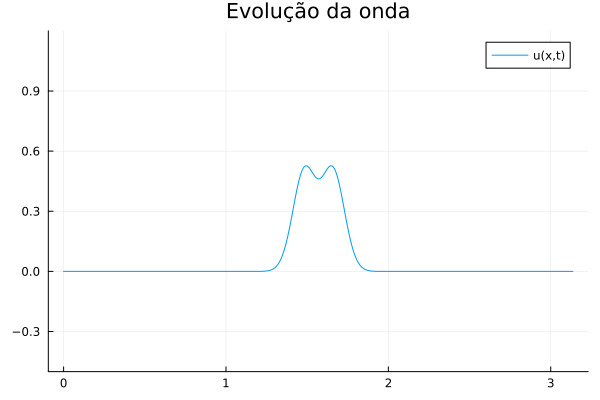
\includegraphics{Trabalho_final_AN_files/gifs/onda0-1}} &
        \adjustbox{max width=\dimexpr\textwidth/3\relax, max height=\dimexpr\textheight/5\relax}{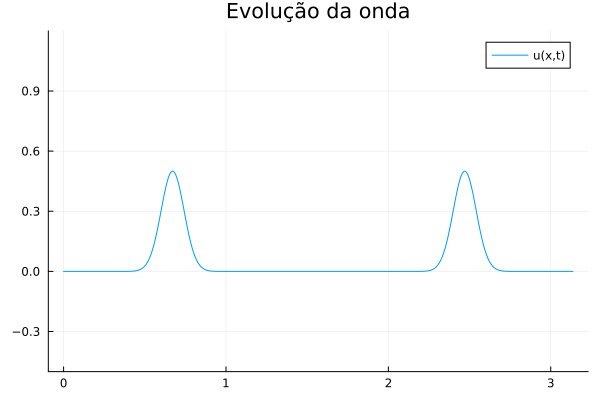
\includegraphics{Trabalho_final_AN_files/gifs/onda0-10}} &
        \adjustbox{max width=\dimexpr\textwidth/3\relax, max height=\dimexpr\textheight/5\relax}{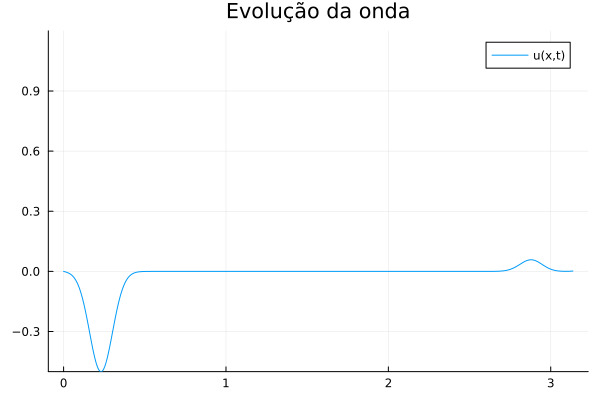
\includegraphics{Trabalho_final_AN_files/gifs/onda0-20}} \\

        % --- Linha 2 ---
        \adjustbox{max width=\dimexpr\textwidth/3\relax, max height=\dimexpr\textheight/5\relax}{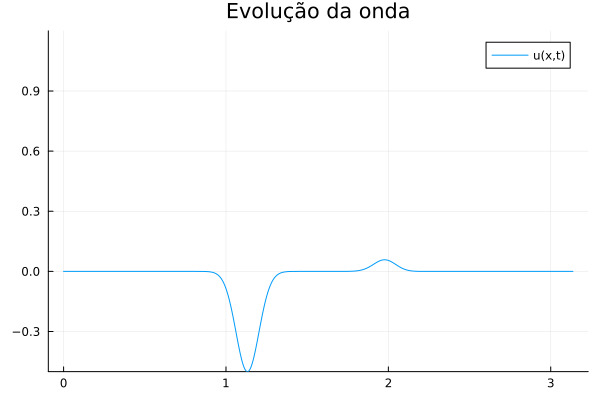
\includegraphics{Trabalho_final_AN_files/gifs/onda0-30}} &
        \adjustbox{max width=\dimexpr\textwidth/3\relax, max height=\dimexpr\textheight/5\relax}{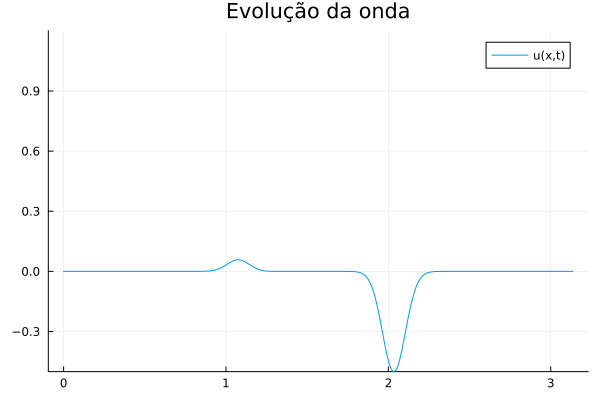
\includegraphics{Trabalho_final_AN_files/gifs/onda0-40}} &
        \adjustbox{max width=\dimexpr\textwidth/3\relax, max height=\dimexpr\textheight/5\relax}{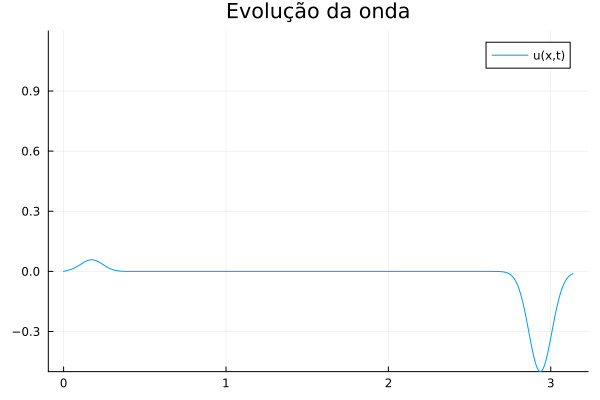
\includegraphics{Trabalho_final_AN_files/gifs/onda0-50}} \\

        % --- Linha 3 ---
        \adjustbox{max width=\dimexpr\textwidth/3\relax, max height=\dimexpr\textheight/5\relax}{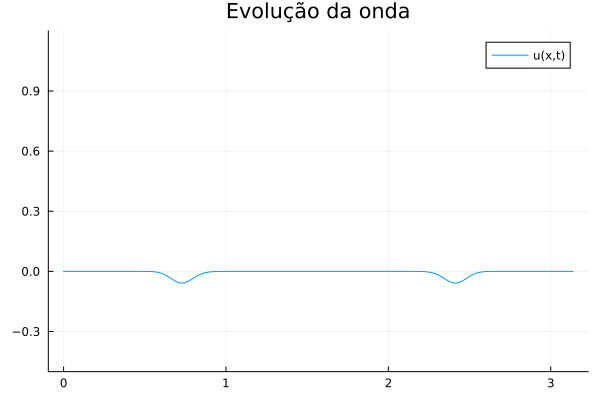
\includegraphics{Trabalho_final_AN_files/gifs/onda0-60}} &
        \adjustbox{max width=\dimexpr\textwidth/3\relax, max height=\dimexpr\textheight/5\relax}{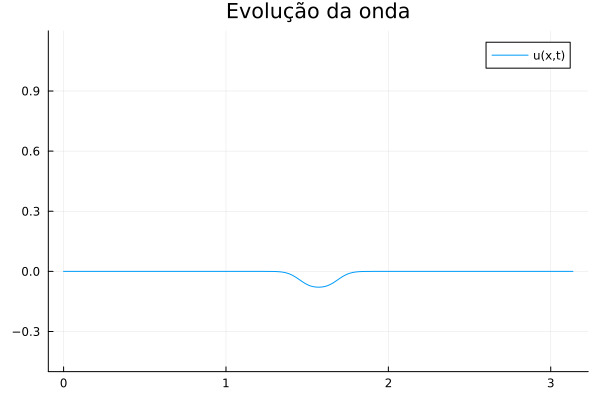
\includegraphics{Trabalho_final_AN_files/gifs/onda0-70}} &
        \adjustbox{max width=\dimexpr\textwidth/3\relax, max height=\dimexpr\textheight/5\relax}{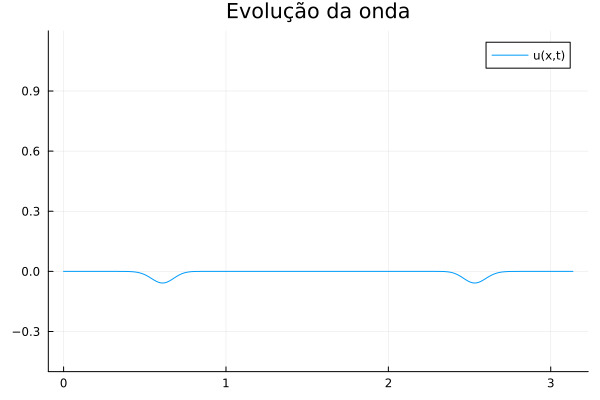
\includegraphics{Trabalho_final_AN_files/gifs/onda0-80}} \\
        
        % --- Linha 4 ---
        \adjustbox{max width=\dimexpr\textwidth/3\relax, max height=\dimexpr\textheight/5\relax}{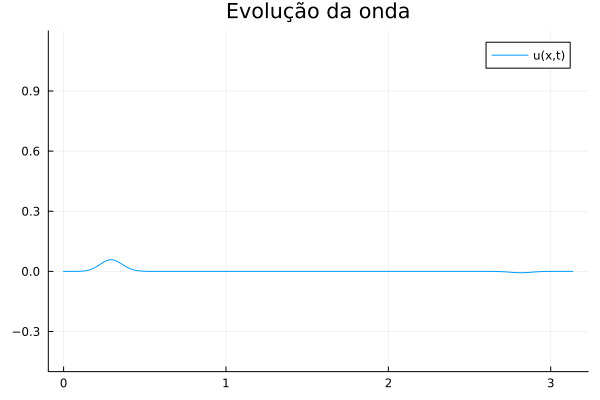
\includegraphics{Trabalho_final_AN_files/gifs/onda0-90}} &
        \adjustbox{max width=\dimexpr\textwidth/3\relax, max height=\dimexpr\textheight/5\relax}{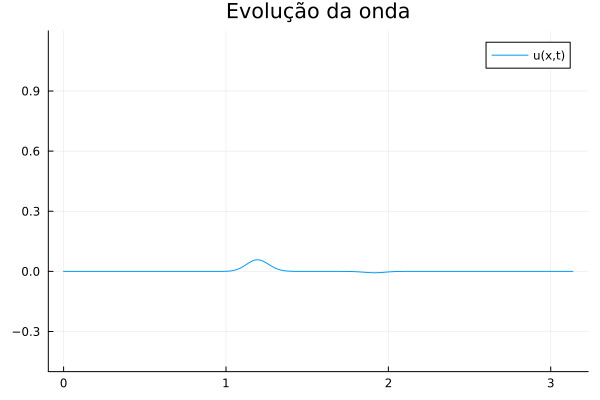
\includegraphics{Trabalho_final_AN_files/gifs/onda0-100}} &
        \adjustbox{max width=\dimexpr\textwidth/3\relax, max height=\dimexpr\textheight/5\relax}{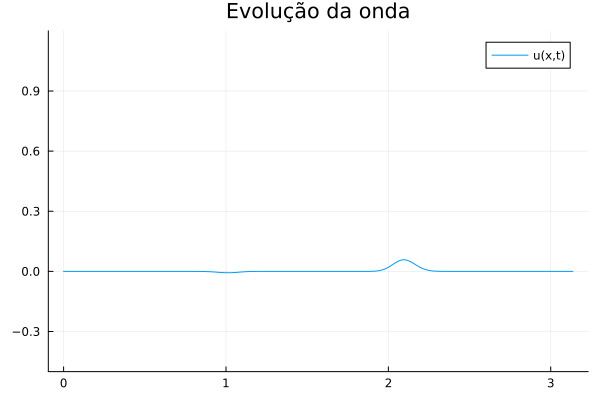
\includegraphics{Trabalho_final_AN_files/gifs/onda0-110}} \\

        % --- Linha 5 ---
        \adjustbox{max width=\dimexpr\textwidth/3\relax, max height=\dimexpr\textheight/5\relax}{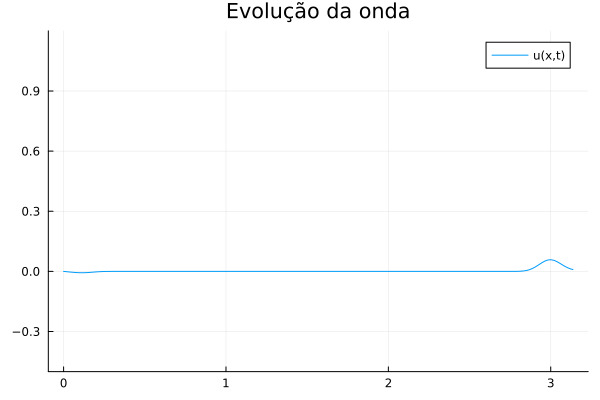
\includegraphics{Trabalho_final_AN_files/gifs/onda0-120}} &
        \adjustbox{max width=\dimexpr\textwidth/3\relax, max height=\dimexpr\textheight/5\relax}{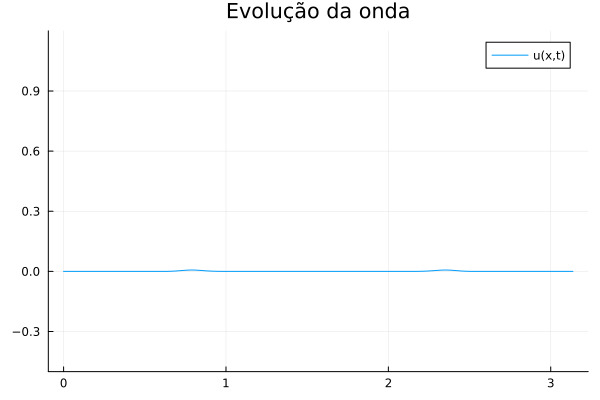
\includegraphics{Trabalho_final_AN_files/gifs/onda0-130}} &
        \adjustbox{max width=\dimexpr\textwidth/3\relax, max height=\dimexpr\textheight/5\relax}{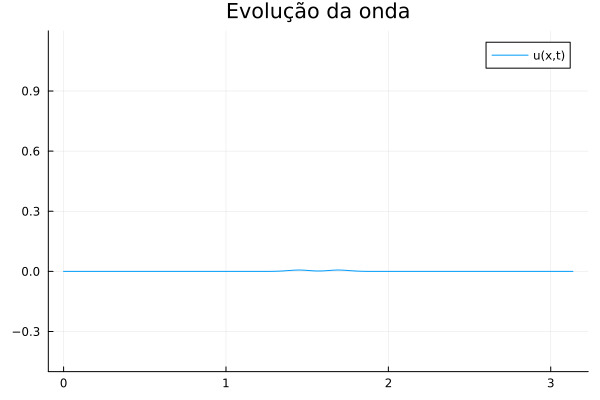
\includegraphics{Trabalho_final_AN_files/gifs/onda0-140}} \\
        
        % Se precisar de 15 imagens, você teria que usar 5 ondas (n=1 a 5) e os 15 frames
        % Os frames seriam: 0, 15, 30, 45, 60, 75, 90, 105, 120, 135, 150, 165, 180, 195, 210, 225

        % Para ter *exatamente* 15 imagens (5x3), precisamos de 15 frames.
        % Os frames solicitados são 0, 15, ..., 225 (16 frames). 
        % Adaptei para 15 frames: 0, 15, ..., 210, utilizando as primeiras 5 ondas. 
        % Para incluir o frame 225, você precisaria de um grid 6x3 ou 5x4.
        
        % Se quiser usar o frame 225, basta adicionar mais uma linha ao \begin{tabular}:
        % --- Linha 6 (Opcional - se o grid fosse 6x3) ---
        % \adjustbox{max width=\dimexpr\textwidth/3\relax, max height=\dimexpr\textheight/5\relax}{\includegraphics{Trabalho_final_AN_files/gifs/onda6-225}} & & \\
        
    \end{tabular}
\end{center}

    \begin{tcolorbox}[breakable, size=fbox, boxrule=1pt, pad at break*=1mm,colback=cellbackground, colframe=cellborder]
\prompt{In}{incolor}{ }{\boxspacing}
\begin{Verbatim}[commandchars=\\\{\}]
\PY{c}{\PYZsh{} LeapFrog}
\PY{n}{δ}\PY{+w}{ }\PY{o}{=}\PY{+w}{ }\PY{l+m+mf}{0.2}\PY{+w}{ }\PY{c}{\PYZsh{} parâmetro de absorção}
\PY{n}{λ}\PY{+w}{ }\PY{o}{=}\PY{+w}{ }\PY{l+m+mf}{0.9}\PY{+w}{ }\PY{c}{\PYZsh{}}
\PY{n}{k}\PY{+w}{ }\PY{o}{=}\PY{+w}{ }\PY{n}{λ}\PY{o}{*}\PY{n}{h}
\PY{n}{T}\PY{+w}{ }\PY{o}{=}\PY{+w}{ }\PY{l+m+mi}{5000}

\PY{n}{U0}\PY{+w}{ }\PY{o}{=}\PY{+w}{  }\PY{n}{f}\PY{o}{.}\PY{p}{(}\PY{n}{domain}\PY{p}{)}\PY{p}{;}
\PY{n}{U1}\PY{+w}{ }\PY{o}{=}\PY{+w}{ }\PY{n}{copy}\PY{p}{(}\PY{n}{U0}\PY{p}{)}\PY{p}{;}\PY{+w}{ }\PY{c}{\PYZsh{} U\PYZca{}1 = U\PYZca{}0}
\PY{n}{U}\PY{+w}{ }\PY{o}{=}\PY{+w}{ }\PY{p}{[}\PY{n}{U0}\PY{p}{,}\PY{+w}{ }\PY{n}{U1}\PY{p}{]}
\PY{n}{M}\PY{+w}{ }\PY{o}{=}\PY{+w}{ }\PY{n}{length}\PY{p}{(}\PY{n}{U0}\PY{p}{)}

\PY{k}{for}\PY{+w}{ }\PY{n}{j}\PY{o}{=}\PY{l+m+mi}{2}\PY{o}{:}\PY{n}{T}
\PY{+w}{  }\PY{n}{Ujp1}\PY{+w}{ }\PY{o}{=}\PY{+w}{ }\PY{n}{zeros}\PY{p}{(}\PY{n}{M}\PY{p}{)}\PY{+w}{ }\PY{c}{\PYZsh{} Ut[0] = 0 por condjção jnjcjal}
\PY{+w}{  }\PY{n}{Uj}\PY{+w}{ }\PY{o}{=}\PY{+w}{ }\PY{n}{U}\PY{p}{[}\PY{n}{j}\PY{p}{]}
\PY{+w}{  }\PY{n}{Ujm1}\PY{+w}{ }\PY{o}{=}\PY{+w}{ }\PY{n}{U}\PY{p}{[}\PY{n}{j}\PY{o}{\PYZhy{}}\PY{l+m+mi}{1}\PY{p}{]}
\PY{+w}{  }\PY{k}{for}\PY{+w}{ }\PY{n}{i}\PY{o}{=}\PY{l+m+mi}{2}\PY{o}{:}\PY{n}{M}\PY{o}{\PYZhy{}}\PY{l+m+mi}{1}\PY{+w}{  }\PY{c}{\PYZsh{} para os pontos jnterjores fazemos o esquema leapfrog}
\PY{+w}{    }\PY{n}{Ujp1}\PY{p}{[}\PY{n}{i}\PY{p}{]}\PY{+w}{ }\PY{o}{=}\PY{+w}{ }\PY{l+m+mi}{2}\PY{n}{Uj}\PY{p}{[}\PY{n}{i}\PY{p}{]}\PY{+w}{ }\PY{o}{\PYZhy{}}\PY{+w}{ }\PY{n}{Ujm1}\PY{p}{[}\PY{n}{i}\PY{p}{]}\PY{+w}{ }\PY{o}{+}\PY{+w}{ }\PY{n}{λ}\PY{o}{\PYZca{}}\PY{l+m+mi}{2}\PY{o}{*}\PY{p}{(}\PY{n}{Uj}\PY{p}{[}\PY{n}{i}\PY{o}{+}\PY{l+m+mi}{1}\PY{p}{]}\PY{o}{+}\PY{n}{Uj}\PY{p}{[}\PY{n}{i}\PY{o}{\PYZhy{}}\PY{l+m+mi}{1}\PY{p}{]}\PY{+w}{ }\PY{o}{\PYZhy{}}\PY{+w}{ }\PY{l+m+mi}{2}\PY{o}{*}\PY{n}{Uj}\PY{p}{[}\PY{n}{i}\PY{p}{]}\PY{p}{)}
\PY{+w}{  }\PY{k}{end}
\PY{+w}{  }\PY{c}{\PYZsh{} e para o ponto da frontejra, usamos uma aproxjmação de 1a ordem}
\PY{+w}{  }\PY{n}{Ujp1}\PY{p}{[}\PY{n}{M}\PY{p}{]}\PY{+w}{ }\PY{o}{=}\PY{+w}{ }\PY{n}{δ}\PY{o}{/}\PY{p}{(}\PY{n}{λ}\PY{o}{+}\PY{n}{δ}\PY{p}{)}\PY{o}{*}\PY{n}{Uj}\PY{p}{[}\PY{n}{M}\PY{p}{]}\PY{+w}{ }\PY{o}{+}\PY{+w}{ }\PY{n}{λ}\PY{o}{/}\PY{p}{(}\PY{n}{λ}\PY{o}{+}\PY{n}{δ}\PY{p}{)}\PY{o}{*}\PY{n}{Ujp1}\PY{p}{[}\PY{n}{M}\PY{o}{\PYZhy{}}\PY{l+m+mi}{1}\PY{p}{]}
\PY{+w}{  }\PY{n}{push!}\PY{p}{(}\PY{n}{U}\PY{p}{,}\PY{+w}{ }\PY{n}{Ujp1}\PY{p}{)}
\PY{k}{end}
\end{Verbatim}
\end{tcolorbox}

    \begin{tcolorbox}[breakable, size=fbox, boxrule=1pt, pad at break*=1mm,colback=cellbackground, colframe=cellborder]
\prompt{In}{incolor}{ }{\boxspacing}
\begin{Verbatim}[commandchars=\\\{\}]
\PY{n+nd}{@gif}\PY{+w}{ }\PY{k}{for}\PY{+w}{ }\PY{n}{t}\PY{o}{=}\PY{l+m+mi}{1}\PY{o}{:}\PY{l+m+mi}{20}\PY{o}{:}\PY{n}{T}
\PY{+w}{  }\PY{n}{plot}\PY{p}{(}\PY{n}{domain}\PY{p}{,}\PY{+w}{ }\PY{n}{U}\PY{p}{[}\PY{n}{t}\PY{p}{]}\PY{p}{,}\PY{+w}{ }\PY{n}{ylim}\PY{o}{=}\PY{p}{(}\PY{o}{\PYZhy{}}\PY{l+m+mf}{0.5}\PY{p}{,}\PY{l+m+mf}{1.2}\PY{p}{)}\PY{p}{,}\PY{+w}{ }\PY{n}{label}\PY{o}{=}\PY{l+s}{\PYZdq{}}\PY{l+s}{u(x,t)}\PY{l+s}{\PYZdq{}}\PY{p}{,}\PY{+w}{ }\PY{n}{title}\PY{o}{=}\PY{l+s}{\PYZdq{}}\PY{l+s}{Evolução da onda}\PY{l+s}{\PYZdq{}}\PY{p}{)}
\PY{k}{end}\PY{+w}{ }\PY{n}{fps}\PY{o}{=}\PY{l+m+mi}{60}
\end{Verbatim}
\end{tcolorbox}
 

        
% Para centralizar a tabela na página
\begin{center}
    % Definimos um array de 3 colunas, todas centralizadas (c)
    % A largura da coluna será automaticamente calculada.
    % A largura total da tabela é ajustada para \textwidth (largura do texto)
    % Ajustamos o espaçamento entre as colunas (colsep) e linhas (rowsep) para ficar mais apertado, se necessário.
    \setlength{\tabcolsep}{1pt} % Espaçamento horizontal entre colunas
    \renewcommand{\arraystretch}{0.5} % Espaçamento vertical entre linhas
    
    \begin{tabular}{ccc} % 3 colunas

        % --- Linha 1 ---
        % As imagens são ajustadas para ter 1/3 da largura do texto menos o espaçamento.
        % Você pode ajustar a escala (\scalebox) se for mais conveniente.
        \adjustbox{max width=\dimexpr\textwidth/3\relax, max height=\dimexpr\textheight/5\relax}{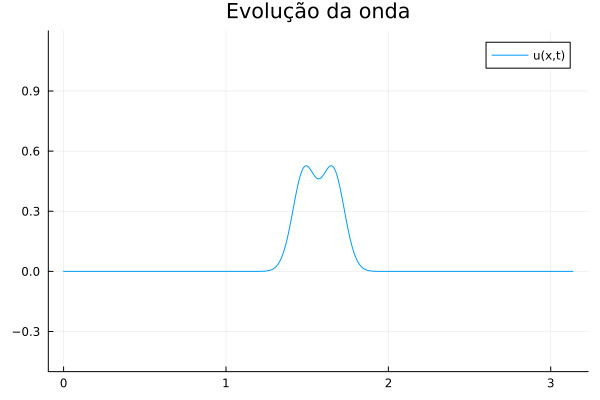
\includegraphics{Trabalho_final_AN_files/gifs/onda1-1}} &
        \adjustbox{max width=\dimexpr\textwidth/3\relax, max height=\dimexpr\textheight/5\relax}{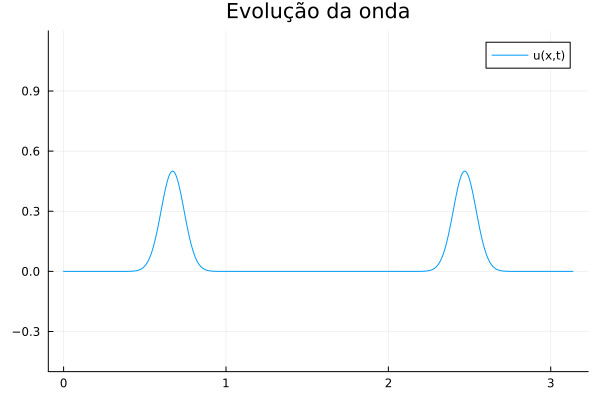
\includegraphics{Trabalho_final_AN_files/gifs/onda1-10}} &
        \adjustbox{max width=\dimexpr\textwidth/3\relax, max height=\dimexpr\textheight/5\relax}{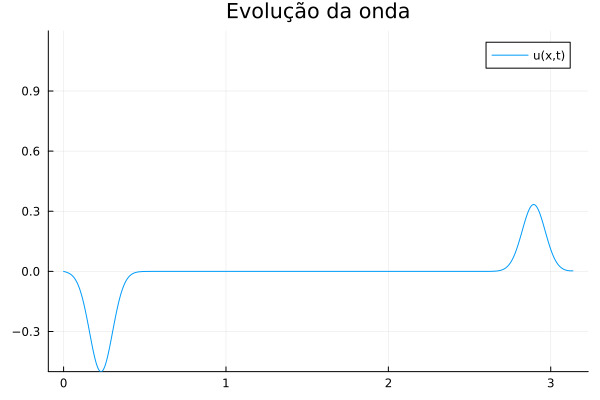
\includegraphics{Trabalho_final_AN_files/gifs/onda1-20}} \\

        % --- Linha 2 ---
        \adjustbox{max width=\dimexpr\textwidth/3\relax, max height=\dimexpr\textheight/5\relax}{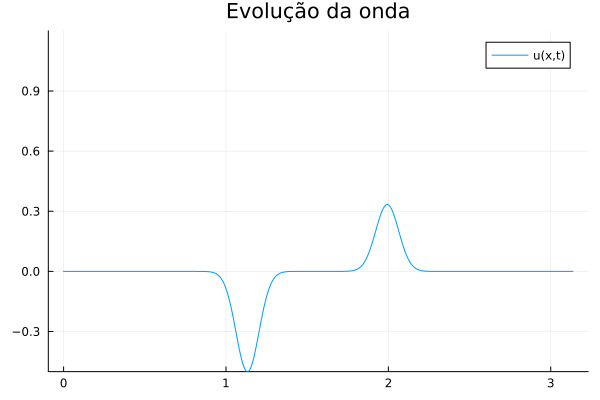
\includegraphics{Trabalho_final_AN_files/gifs/onda1-30}} &
        \adjustbox{max width=\dimexpr\textwidth/3\relax, max height=\dimexpr\textheight/5\relax}{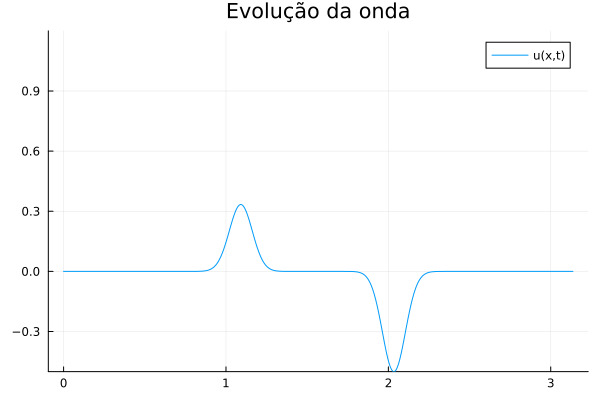
\includegraphics{Trabalho_final_AN_files/gifs/onda1-40}} &
        \adjustbox{max width=\dimexpr\textwidth/3\relax, max height=\dimexpr\textheight/5\relax}{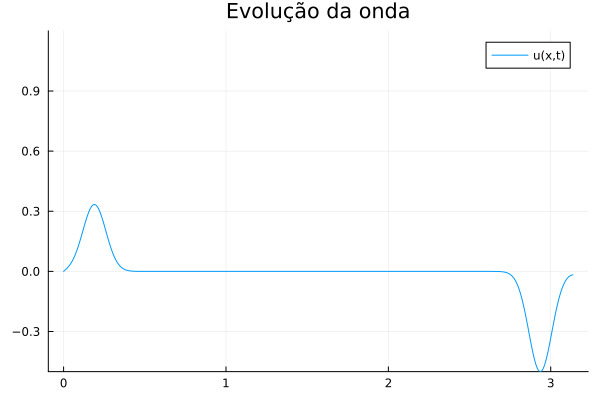
\includegraphics{Trabalho_final_AN_files/gifs/onda1-50}} \\

        % --- Linha 3 ---
        \adjustbox{max width=\dimexpr\textwidth/3\relax, max height=\dimexpr\textheight/5\relax}{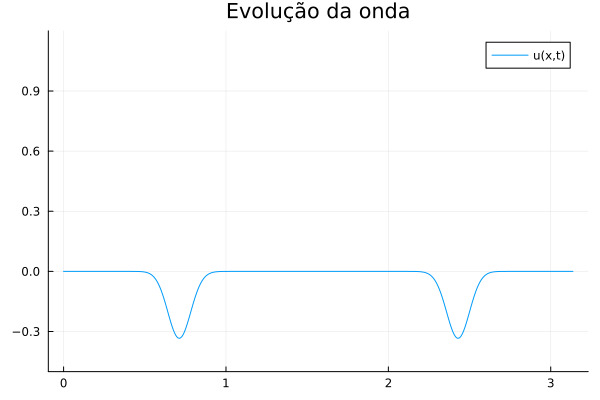
\includegraphics{Trabalho_final_AN_files/gifs/onda1-60}} &
        \adjustbox{max width=\dimexpr\textwidth/3\relax, max height=\dimexpr\textheight/5\relax}{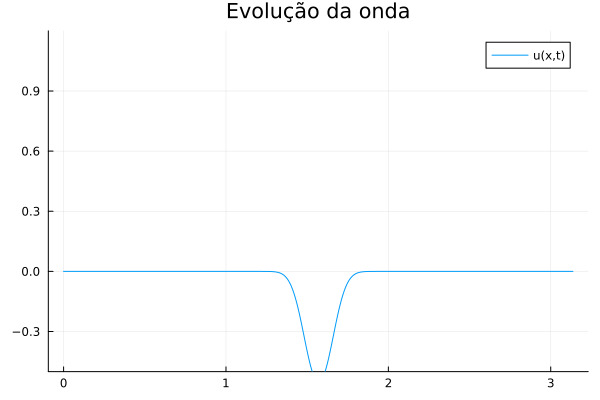
\includegraphics{Trabalho_final_AN_files/gifs/onda1-70}} &
        \adjustbox{max width=\dimexpr\textwidth/3\relax, max height=\dimexpr\textheight/5\relax}{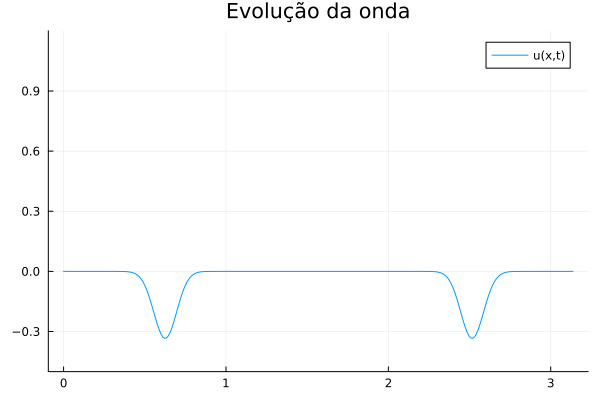
\includegraphics{Trabalho_final_AN_files/gifs/onda1-80}} \\
        
        % --- Linha 4 ---
        \adjustbox{max width=\dimexpr\textwidth/3\relax, max height=\dimexpr\textheight/5\relax}{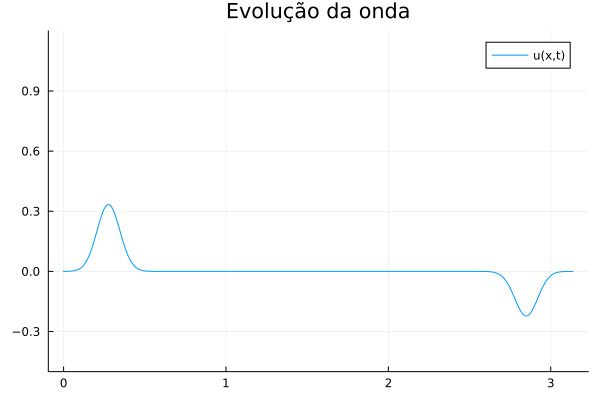
\includegraphics{Trabalho_final_AN_files/gifs/onda1-90}} &
        \adjustbox{max width=\dimexpr\textwidth/3\relax, max height=\dimexpr\textheight/5\relax}{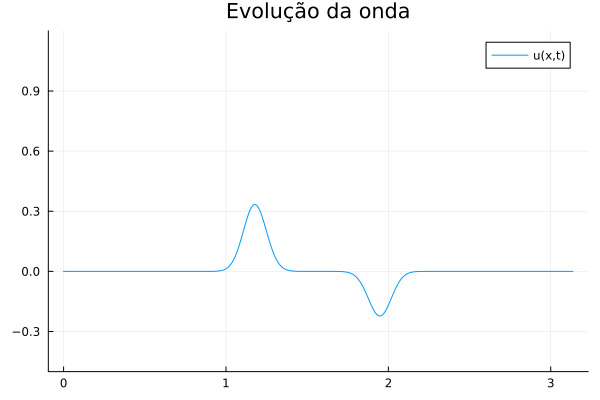
\includegraphics{Trabalho_final_AN_files/gifs/onda1-100}} &
        \adjustbox{max width=\dimexpr\textwidth/3\relax, max height=\dimexpr\textheight/5\relax}{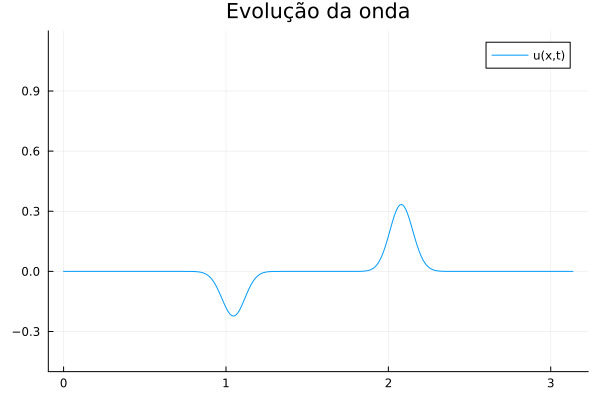
\includegraphics{Trabalho_final_AN_files/gifs/onda1-110}} \\

        % --- Linha 5 ---
        \adjustbox{max width=\dimexpr\textwidth/3\relax, max height=\dimexpr\textheight/5\relax}{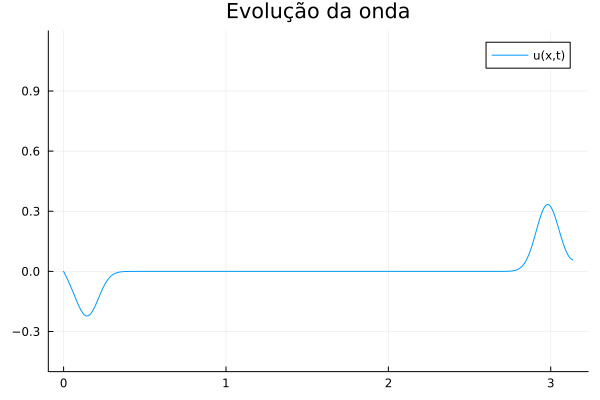
\includegraphics{Trabalho_final_AN_files/gifs/onda1-120}} &
        \adjustbox{max width=\dimexpr\textwidth/3\relax, max height=\dimexpr\textheight/5\relax}{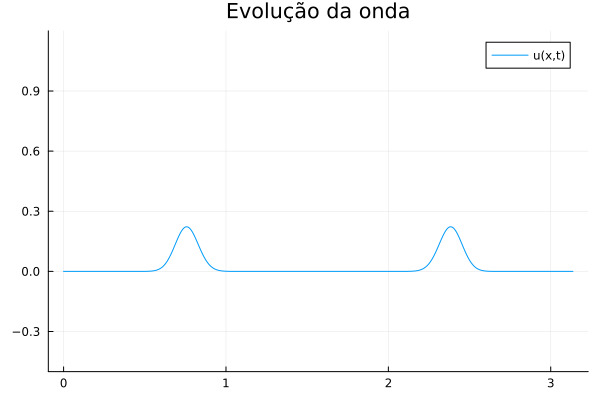
\includegraphics{Trabalho_final_AN_files/gifs/onda1-130}} &
        \adjustbox{max width=\dimexpr\textwidth/3\relax, max height=\dimexpr\textheight/5\relax}{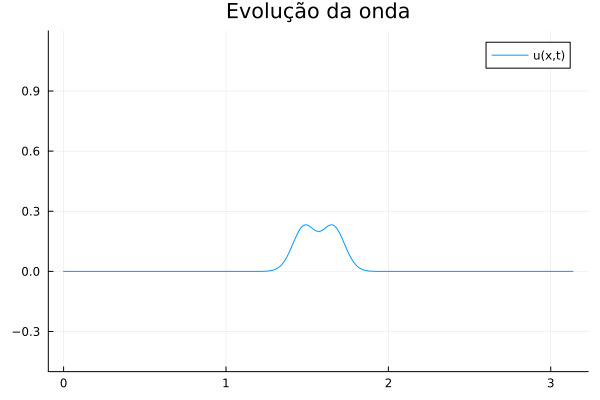
\includegraphics{Trabalho_final_AN_files/gifs/onda1-140}} \\
        
        % Se precisar de 15 imagens, você teria que usar 5 ondas (n=1 a 5) e os 15 frames
        % Os frames seriam: 0, 15, 30, 45, 60, 75, 90, 105, 120, 135, 150, 165, 180, 195, 210, 225

        % Para ter *exatamente* 15 imagens (5x3), precisamos de 15 frames.
        % Os frames solicitados são 0, 15, ..., 225 (16 frames). 
        % Adaptei para 15 frames: 0, 15, ..., 210, utilizando as primeiras 5 ondas. 
        % Para incluir o frame 225, você precisaria de um grid 6x3 ou 5x4.
        
        % Se quiser usar o frame 225, basta adicionar mais uma linha ao \begin{tabular}:
        % --- Linha 6 (Opcional - se o grid fosse 6x3) ---
        % \adjustbox{max width=\dimexpr\textwidth/3\relax, max height=\dimexpr\textheight/5\relax}{\includegraphics{Trabalho_final_AN_files/gifs/onda6-225}} & & \\
        
    \end{tabular}
\end{center}

    Veja que o parâmetro \(\delta=0.8\) causou um efeito maior de absorção,
enquanto um \(\delta=0.2\) causou um efeito maior de reflexão.

    \hypertarget{muxe9todo-box}{%
\subsubsection{Método Box}\label{muxe9todo-box}}

A equação da onda: \[ u_{tt} - u_{xx} = 0 \]

Defina: \[ v = u_t \quad \text{e} \quad w = u_x \]

Então temos o sistema: \[ \begin{cases}
v_t - w_x = 0 \\
w_t - v_x = 0
\end{cases} \]

\hypertarget{condiuxe7uxf5es-iniciais-e-de-contorno}{%
\subsubsection{Condições Iniciais e de
Contorno}\label{condiuxe7uxf5es-iniciais-e-de-contorno}}

Condições iniciais: \[ u(x,0) = \exp(-100(x-\pi/2)^2) \]
\[ v(x,0) = u_t(x,0) = 0 \]
\[ w(x,0) = u_x(x,0) = -200(x-\pi/2)\exp(-100(x-\pi/2)^2) \]

Condições de contorno: \[ u(0,t) = 0 \Rightarrow v(0,t) = 0 \]
\[ u_x(\pi,t) + \delta u_t(\pi,t) = 0 \Rightarrow w(\pi,t) + \delta v(\pi,t) = 0 \]

\hypertarget{discretizauxe7uxe3o-com-muxe9todo-box}{%
\subsubsection{Discretização com Método
Box}\label{discretizauxe7uxe3o-com-muxe9todo-box}}

Em cada direção, calculamos a média das aproximações por diferenças
progressivas.

\textbf{Equação 1 \(v_t - w_x = 0\):}
\[ \frac{V_{i+1,j+1} - V_{i+1,j}+ V_{i,j+1} - V_{i,j}}{2k} - \frac{W_{i+1,j+1} - W_{i,j+1} + W_{i+1,j} - W_{i,j}}{2h} = 0 \]

\textbf{Equação 2 \(w_t - v_x = 0\):}
\[ \frac{W_{i+1,j+1} - W_{i+1,j} + W_{i,j+1} - W_{i,j}}{2k} - \frac{V_{i+1,j+1} - V_{i,j+1} + V_{i+1,j} - V_{i,j}}{2h} = 0 \]

Onde: - \$ V\_\{i,j\} = v(x\_i, t\_j) \$, - \$ W\_\{i,j\} = w(x\_i,
t\_j) \$,

\hypertarget{sistema-linear-para-cada-passo-de-tempo}{%
\subsubsection{Sistema Linear para Cada Passo de
Tempo}\label{sistema-linear-para-cada-passo-de-tempo}}

Para cada passo no tempo, montamos um sistema linear
\[A\mathbf{U}^{j+1} = \mathbf{b},\] onde:
\[ \mathbf{U}^{j+1} = [v_0, w_0, v_1, w_1, \ldots, v_N, w_N]^T \]

    \begin{tcolorbox}[breakable, size=fbox, boxrule=1pt, pad at break*=1mm,colback=cellbackground, colframe=cellborder]
\prompt{In}{incolor}{ }{\boxspacing}
\begin{Verbatim}[commandchars=\\\{\}]
\PY{c}{\PYZsh{} Box}
\PY{n}{δ}\PY{+w}{ }\PY{o}{=}\PY{+w}{ }\PY{l+m+mf}{0.8}\PY{+w}{ }\PY{c}{\PYZsh{} parâmetro de absorção}
\PY{n}{λ}\PY{+w}{ }\PY{o}{=}\PY{+w}{ }\PY{l+m+mf}{0.9}\PY{+w}{ }\PY{c}{\PYZsh{}}
\PY{n}{k}\PY{+w}{ }\PY{o}{=}\PY{+w}{ }\PY{n}{λ}\PY{o}{*}\PY{n}{h}

\PY{n}{T}\PY{+w}{ }\PY{o}{=}\PY{+w}{ }\PY{l+m+mi}{4000}

\PY{n}{U0}\PY{+w}{ }\PY{o}{=}\PY{+w}{  }\PY{n}{f}\PY{o}{.}\PY{p}{(}\PY{n}{domain}\PY{p}{)}\PY{p}{;}
\PY{n}{U1}\PY{+w}{ }\PY{o}{=}\PY{+w}{ }\PY{n}{copy}\PY{p}{(}\PY{n}{U0}\PY{p}{)}\PY{p}{;}\PY{+w}{ }\PY{c}{\PYZsh{} U\PYZca{}1 = U\PYZca{}0}
\PY{n}{U}\PY{+w}{ }\PY{o}{=}\PY{+w}{ }\PY{p}{[}\PY{n}{U0}\PY{p}{,}\PY{+w}{ }\PY{n}{U1}\PY{p}{]}
\PY{n}{M}\PY{+w}{ }\PY{o}{=}\PY{+w}{ }\PY{n}{length}\PY{p}{(}\PY{n}{U0}\PY{p}{)}


\PY{k}{function}\PY{+w}{ }\PY{n}{w}\PY{p}{(}\PY{n}{x}\PY{p}{)}\PY{+w}{ }\PY{c}{\PYZsh{}u\PYZus{}x}
\PY{+w}{    }\PY{k}{return}\PY{+w}{ }\PY{o}{\PYZhy{}}\PY{l+m+mi}{200}\PY{o}{*}\PY{p}{(}\PY{n}{x}\PY{+w}{ }\PY{o}{\PYZhy{}}\PY{+w}{ }\PY{n+nb}{π}\PY{o}{/}\PY{l+m+mi}{2}\PY{p}{)}\PY{+w}{ }\PY{o}{*}\PY{+w}{ }\PY{n}{exp}\PY{p}{(}\PY{o}{\PYZhy{}}\PY{l+m+mi}{100}\PY{o}{*}\PY{p}{(}\PY{n}{x}\PY{+w}{ }\PY{o}{\PYZhy{}}\PY{+w}{ }\PY{n+nb}{π}\PY{o}{/}\PY{l+m+mi}{2}\PY{p}{)}\PY{o}{\PYZca{}}\PY{l+m+mi}{2}\PY{p}{)}
\PY{k}{end}

\PY{n}{V}\PY{+w}{ }\PY{o}{=}\PY{+w}{ }\PY{p}{[}\PY{n}{zeros}\PY{p}{(}\PY{n}{M}\PY{p}{)}\PY{p}{]}
\PY{n}{W}\PY{+w}{ }\PY{o}{=}\PY{+w}{ }\PY{p}{[}\PY{n}{w}\PY{o}{.}\PY{p}{(}\PY{n}{domain}\PY{p}{)}\PY{p}{]}

\PY{n}{ν}\PY{+w}{ }\PY{o}{=}\PY{+w}{ }\PY{n}{k}\PY{+w}{ }\PY{o}{/}\PY{+w}{ }\PY{n}{h}


\PY{c}{\PYZsh{} Método Box para a equação da onda}

\PY{k}{for}\PY{+w}{ }\PY{n}{j}\PY{o}{=}\PY{l+m+mi}{1}\PY{o}{:}\PY{n}{T}

\PY{+w}{    }\PY{n}{Vj}\PY{+w}{ }\PY{o}{=}\PY{+w}{ }\PY{n}{V}\PY{p}{[}\PY{n}{j}\PY{p}{]}
\PY{+w}{    }\PY{n}{Wj}\PY{+w}{ }\PY{o}{=}\PY{+w}{ }\PY{n}{W}\PY{p}{[}\PY{n}{j}\PY{p}{]}
\PY{+w}{    }\PY{n}{Uj}\PY{+w}{ }\PY{o}{=}\PY{+w}{ }\PY{n}{U}\PY{p}{[}\PY{n}{j}\PY{o}{+}\PY{l+m+mi}{1}\PY{p}{]}
\PY{+w}{    }\PY{c}{\PYZsh{} Montar sistema linear A * U\PYZus{}\PYZob{}j+1\PYZcb{} = b}

\PY{+w}{    }\PY{c}{\PYZsh{} Número de equações:}
\PY{+w}{    }\PY{c}{\PYZsh{} 2 equações para cada intervalo}
\PY{+w}{    }\PY{c}{\PYZsh{} + 2 condições de contorno \PYZhy{}\PYZgt{} total 2(M) = 2(N+1)}
\PY{+w}{    }\PY{n}{n\PYZus{}equations}\PY{+w}{ }\PY{o}{=}\PY{+w}{ }\PY{l+m+mi}{2}\PY{o}{*}\PY{n}{M}
\PY{+w}{    }\PY{n}{A}\PY{+w}{ }\PY{o}{=}\PY{+w}{ }\PY{n}{spzeros}\PY{p}{(}\PY{n}{n\PYZus{}equations}\PY{p}{,}\PY{+w}{ }\PY{n}{n\PYZus{}equations}\PY{p}{)}
\PY{+w}{    }\PY{n}{b}\PY{+w}{ }\PY{o}{=}\PY{+w}{ }\PY{n}{zeros}\PY{p}{(}\PY{n}{n\PYZus{}equations}\PY{p}{)}

\PY{+w}{    }\PY{n}{eq\PYZus{}counter}\PY{+w}{ }\PY{o}{=}\PY{+w}{ }\PY{l+m+mi}{0}

\PY{+w}{    }\PY{c}{\PYZsh{} Condição de contorno em x=0: v(0,t)=0}
\PY{+w}{    }\PY{n}{eq\PYZus{}counter}\PY{+w}{ }\PY{o}{+=}\PY{+w}{ }\PY{l+m+mi}{1}
\PY{+w}{    }\PY{n}{A}\PY{p}{[}\PY{n}{eq\PYZus{}counter}\PY{p}{,}\PY{+w}{ }\PY{l+m+mi}{1}\PY{p}{]}\PY{+w}{ }\PY{o}{=}\PY{+w}{ }\PY{l+m+mf}{1.0}\PY{+w}{  }\PY{c}{\PYZsh{} v\PYZus{}0}
\PY{+w}{    }\PY{n}{b}\PY{p}{[}\PY{n}{eq\PYZus{}counter}\PY{p}{]}\PY{+w}{ }\PY{o}{=}\PY{+w}{ }\PY{l+m+mf}{0.0}

\PY{+w}{    }\PY{c}{\PYZsh{} Equações para cada intervalo interno (i=1:N)}
\PY{+w}{    }\PY{k}{for}\PY{+w}{ }\PY{n}{i}\PY{+w}{ }\PY{k}{in}\PY{+w}{ }\PY{l+m+mi}{1}\PY{o}{:}\PY{n}{M}\PY{o}{\PYZhy{}}\PY{l+m+mi}{1}
\PY{+w}{        }\PY{c}{\PYZsh{} Equação 1 para o intervalo (i, i+1)}
\PY{+w}{        }\PY{n}{eq\PYZus{}counter}\PY{+w}{ }\PY{o}{+=}\PY{+w}{ }\PY{l+m+mi}{1}
\PY{+w}{        }\PY{c}{\PYZsh{} Coeficientes para v\PYZus{}i, v\PYZus{}\PYZob{}i+1\PYZcb{}, w\PYZus{}i, w\PYZus{}\PYZob{}i+1\PYZcb{}}
\PY{+w}{        }\PY{n}{v\PYZus{}i\PYZus{}idx}\PY{+w}{ }\PY{o}{=}\PY{+w}{ }\PY{l+m+mi}{2}\PY{o}{*}\PY{p}{(}\PY{n}{i}\PY{o}{\PYZhy{}}\PY{l+m+mi}{1}\PY{p}{)}\PY{+w}{ }\PY{o}{+}\PY{+w}{ }\PY{l+m+mi}{1}
\PY{+w}{        }\PY{n}{w\PYZus{}i\PYZus{}idx}\PY{+w}{ }\PY{o}{=}\PY{+w}{ }\PY{l+m+mi}{2}\PY{o}{*}\PY{p}{(}\PY{n}{i}\PY{o}{\PYZhy{}}\PY{l+m+mi}{1}\PY{p}{)}\PY{+w}{ }\PY{o}{+}\PY{+w}{ }\PY{l+m+mi}{2}
\PY{+w}{        }\PY{n}{v\PYZus{}ip1\PYZus{}idx}\PY{+w}{ }\PY{o}{=}\PY{+w}{ }\PY{l+m+mi}{2}\PY{o}{*}\PY{n}{i}\PY{+w}{ }\PY{o}{+}\PY{+w}{ }\PY{l+m+mi}{1}
\PY{+w}{        }\PY{n}{w\PYZus{}ip1\PYZus{}idx}\PY{+w}{ }\PY{o}{=}\PY{+w}{ }\PY{l+m+mi}{2}\PY{o}{*}\PY{n}{i}\PY{+w}{ }\PY{o}{+}\PY{+w}{ }\PY{l+m+mi}{2}

\PY{+w}{        }\PY{c}{\PYZsh{} v\PYZus{}i + v\PYZus{}\PYZob{}i+1\PYZcb{} + ν*w\PYZus{}i \PYZhy{} ν*w\PYZus{}\PYZob{}i+1\PYZcb{} = R\PYZus{}v}
\PY{+w}{        }\PY{n}{A}\PY{p}{[}\PY{n}{eq\PYZus{}counter}\PY{p}{,}\PY{+w}{ }\PY{n}{v\PYZus{}i\PYZus{}idx}\PY{p}{]}\PY{+w}{ }\PY{o}{=}\PY{+w}{ }\PY{l+m+mf}{1.0}
\PY{+w}{        }\PY{n}{A}\PY{p}{[}\PY{n}{eq\PYZus{}counter}\PY{p}{,}\PY{+w}{ }\PY{n}{v\PYZus{}ip1\PYZus{}idx}\PY{p}{]}\PY{+w}{ }\PY{o}{=}\PY{+w}{ }\PY{l+m+mf}{1.0}
\PY{+w}{        }\PY{n}{A}\PY{p}{[}\PY{n}{eq\PYZus{}counter}\PY{p}{,}\PY{+w}{ }\PY{n}{w\PYZus{}i\PYZus{}idx}\PY{p}{]}\PY{+w}{ }\PY{o}{=}\PY{+w}{ }\PY{n}{ν}
\PY{+w}{        }\PY{n}{A}\PY{p}{[}\PY{n}{eq\PYZus{}counter}\PY{p}{,}\PY{+w}{ }\PY{n}{w\PYZus{}ip1\PYZus{}idx}\PY{p}{]}\PY{+w}{ }\PY{o}{=}\PY{+w}{ }\PY{o}{\PYZhy{}}\PY{n}{ν}

\PY{+w}{        }\PY{c}{\PYZsh{} Lado direito R\PYZus{}v}
\PY{+w}{        }\PY{n}{R\PYZus{}v}\PY{+w}{ }\PY{o}{=}\PY{+w}{ }\PY{n}{Vj}\PY{p}{[}\PY{n}{i}\PY{p}{]}\PY{+w}{ }\PY{o}{+}\PY{+w}{ }\PY{n}{Vj}\PY{p}{[}\PY{n}{i}\PY{o}{+}\PY{l+m+mi}{1}\PY{p}{]}\PY{+w}{ }\PY{o}{+}\PY{+w}{ }\PY{n}{ν}\PY{o}{*}\PY{p}{(}\PY{n}{Wj}\PY{p}{[}\PY{n}{i}\PY{o}{+}\PY{l+m+mi}{1}\PY{p}{]}\PY{+w}{ }\PY{o}{\PYZhy{}}\PY{+w}{ }\PY{n}{Wj}\PY{p}{[}\PY{n}{i}\PY{p}{]}\PY{p}{)}
\PY{+w}{        }\PY{n}{b}\PY{p}{[}\PY{n}{eq\PYZus{}counter}\PY{p}{]}\PY{+w}{ }\PY{o}{=}\PY{+w}{ }\PY{n}{R\PYZus{}v}

\PY{+w}{        }\PY{c}{\PYZsh{} Equação 2 para o intervalo (i, i+1)}
\PY{+w}{        }\PY{n}{eq\PYZus{}counter}\PY{+w}{ }\PY{o}{+=}\PY{+w}{ }\PY{l+m+mi}{1}
\PY{+w}{        }\PY{c}{\PYZsh{} w\PYZus{}i + w\PYZus{}\PYZob{}i+1\PYZcb{} + ν*v\PYZus{}i \PYZhy{} ν*v\PYZus{}\PYZob{}i+1\PYZcb{} = R\PYZus{}w}
\PY{+w}{        }\PY{n}{A}\PY{p}{[}\PY{n}{eq\PYZus{}counter}\PY{p}{,}\PY{+w}{ }\PY{n}{w\PYZus{}i\PYZus{}idx}\PY{p}{]}\PY{+w}{ }\PY{o}{=}\PY{+w}{ }\PY{l+m+mf}{1.0}
\PY{+w}{        }\PY{n}{A}\PY{p}{[}\PY{n}{eq\PYZus{}counter}\PY{p}{,}\PY{+w}{ }\PY{n}{w\PYZus{}ip1\PYZus{}idx}\PY{p}{]}\PY{+w}{ }\PY{o}{=}\PY{+w}{ }\PY{l+m+mf}{1.0}
\PY{+w}{        }\PY{n}{A}\PY{p}{[}\PY{n}{eq\PYZus{}counter}\PY{p}{,}\PY{+w}{ }\PY{n}{v\PYZus{}i\PYZus{}idx}\PY{p}{]}\PY{+w}{ }\PY{o}{=}\PY{+w}{ }\PY{n}{ν}
\PY{+w}{        }\PY{n}{A}\PY{p}{[}\PY{n}{eq\PYZus{}counter}\PY{p}{,}\PY{+w}{ }\PY{n}{v\PYZus{}ip1\PYZus{}idx}\PY{p}{]}\PY{+w}{ }\PY{o}{=}\PY{+w}{ }\PY{o}{\PYZhy{}}\PY{n}{ν}

\PY{+w}{        }\PY{c}{\PYZsh{} Lado direito R\PYZus{}w}
\PY{+w}{        }\PY{n}{R\PYZus{}w}\PY{+w}{ }\PY{o}{=}\PY{+w}{ }\PY{n}{Wj}\PY{p}{[}\PY{n}{i}\PY{p}{]}\PY{+w}{ }\PY{o}{+}\PY{+w}{ }\PY{n}{Wj}\PY{p}{[}\PY{n}{i}\PY{o}{+}\PY{l+m+mi}{1}\PY{p}{]}\PY{+w}{ }\PY{o}{+}\PY{+w}{ }\PY{n}{ν}\PY{o}{*}\PY{p}{(}\PY{n}{Vj}\PY{p}{[}\PY{n}{i}\PY{o}{+}\PY{l+m+mi}{1}\PY{p}{]}\PY{+w}{ }\PY{o}{\PYZhy{}}\PY{+w}{ }\PY{n}{Vj}\PY{p}{[}\PY{n}{i}\PY{p}{]}\PY{p}{)}
\PY{+w}{        }\PY{n}{b}\PY{p}{[}\PY{n}{eq\PYZus{}counter}\PY{p}{]}\PY{+w}{ }\PY{o}{=}\PY{+w}{ }\PY{n}{R\PYZus{}w}
\PY{+w}{    }\PY{k}{end}

\PY{+w}{    }\PY{c}{\PYZsh{} Condição de contorno em x=π: w\PYZus{}N + δ*v\PYZus{}N = 0}
\PY{+w}{    }\PY{n}{eq\PYZus{}counter}\PY{+w}{ }\PY{o}{+=}\PY{+w}{ }\PY{l+m+mi}{1}
\PY{+w}{    }\PY{n}{v\PYZus{}N\PYZus{}idx}\PY{+w}{ }\PY{o}{=}\PY{+w}{ }\PY{l+m+mi}{2}\PY{o}{*}\PY{p}{(}\PY{n}{M}\PY{o}{\PYZhy{}}\PY{l+m+mi}{1}\PY{p}{)}\PY{+w}{ }\PY{o}{+}\PY{+w}{ }\PY{l+m+mi}{1}
\PY{+w}{    }\PY{n}{w\PYZus{}N\PYZus{}idx}\PY{+w}{ }\PY{o}{=}\PY{+w}{ }\PY{l+m+mi}{2}\PY{o}{*}\PY{p}{(}\PY{n}{M}\PY{o}{\PYZhy{}}\PY{l+m+mi}{1}\PY{p}{)}\PY{+w}{ }\PY{o}{+}\PY{+w}{ }\PY{l+m+mi}{2}
\PY{+w}{    }\PY{n}{A}\PY{p}{[}\PY{n}{eq\PYZus{}counter}\PY{p}{,}\PY{+w}{ }\PY{n}{v\PYZus{}N\PYZus{}idx}\PY{p}{]}\PY{+w}{ }\PY{o}{=}\PY{+w}{ }\PY{n}{δ}
\PY{+w}{    }\PY{n}{A}\PY{p}{[}\PY{n}{eq\PYZus{}counter}\PY{p}{,}\PY{+w}{ }\PY{n}{w\PYZus{}N\PYZus{}idx}\PY{p}{]}\PY{+w}{ }\PY{o}{=}\PY{+w}{ }\PY{l+m+mf}{1.0}
\PY{+w}{    }\PY{n}{b}\PY{p}{[}\PY{n}{eq\PYZus{}counter}\PY{p}{]}\PY{+w}{ }\PY{o}{=}\PY{+w}{ }\PY{l+m+mf}{0.0}

\PY{+w}{    }\PY{c}{\PYZsh{} Resolver sistema linear}
\PY{+w}{    }\PY{n}{U\PYZus{}next}\PY{+w}{ }\PY{o}{=}\PY{+w}{ }\PY{n}{A}\PY{+w}{ }\PY{o}{\PYZbs{}}\PY{+w}{ }\PY{n}{b}

\PY{+w}{    }\PY{c}{\PYZsh{} Extrair soluções}
\PY{+w}{    }\PY{n}{Vjp1}\PY{+w}{ }\PY{o}{=}\PY{+w}{ }\PY{n}{zeros}\PY{p}{(}\PY{n}{M}\PY{p}{)}
\PY{+w}{    }\PY{n}{Wjp1}\PY{+w}{ }\PY{o}{=}\PY{+w}{ }\PY{n}{zeros}\PY{p}{(}\PY{n}{M}\PY{p}{)}
\PY{+w}{    }\PY{k}{for}\PY{+w}{ }\PY{n}{i}\PY{+w}{ }\PY{k}{in}\PY{+w}{ }\PY{l+m+mi}{1}\PY{o}{:}\PY{n}{M}
\PY{+w}{        }\PY{n}{Vjp1}\PY{p}{[}\PY{n}{i}\PY{p}{]}\PY{+w}{ }\PY{o}{=}\PY{+w}{ }\PY{n}{U\PYZus{}next}\PY{p}{[}\PY{l+m+mi}{2}\PY{o}{*}\PY{p}{(}\PY{n}{i}\PY{o}{\PYZhy{}}\PY{l+m+mi}{1}\PY{p}{)}\PY{o}{+}\PY{l+m+mi}{1}\PY{p}{]}
\PY{+w}{        }\PY{n}{Wjp1}\PY{p}{[}\PY{n}{i}\PY{p}{]}\PY{+w}{ }\PY{o}{=}\PY{+w}{ }\PY{n}{U\PYZus{}next}\PY{p}{[}\PY{l+m+mi}{2}\PY{o}{*}\PY{p}{(}\PY{n}{i}\PY{o}{\PYZhy{}}\PY{l+m+mi}{1}\PY{p}{)}\PY{o}{+}\PY{l+m+mi}{2}\PY{p}{]}
\PY{+w}{    }\PY{k}{end}

\PY{+w}{    }\PY{n}{push!}\PY{p}{(}\PY{n}{V}\PY{p}{,}\PY{+w}{ }\PY{n}{Vjp1}\PY{p}{)}
\PY{+w}{    }\PY{n}{push!}\PY{p}{(}\PY{n}{W}\PY{p}{,}\PY{+w}{ }\PY{n}{Wjp1}\PY{p}{)}

\PY{+w}{    }\PY{c}{\PYZsh{} Atualizar u usando regra do trapézio}
\PY{+w}{    }\PY{n}{Ujp1}\PY{+w}{ }\PY{o}{=}\PY{+w}{ }\PY{n}{zeros}\PY{p}{(}\PY{n}{M}\PY{p}{)}
\PY{+w}{    }\PY{k}{for}\PY{+w}{ }\PY{n}{i}\PY{+w}{ }\PY{k}{in}\PY{+w}{ }\PY{l+m+mi}{1}\PY{o}{:}\PY{n}{M}
\PY{+w}{        }\PY{n}{Ujp1}\PY{p}{[}\PY{n}{i}\PY{p}{]}\PY{+w}{ }\PY{o}{=}\PY{+w}{ }\PY{n}{Uj}\PY{p}{[}\PY{n}{i}\PY{p}{]}\PY{+w}{ }\PY{o}{+}\PY{+w}{ }\PY{p}{(}\PY{n}{k}\PY{o}{/}\PY{l+m+mi}{2}\PY{p}{)}\PY{o}{*}\PY{p}{(}\PY{n}{Vj}\PY{p}{[}\PY{n}{i}\PY{p}{]}\PY{+w}{ }\PY{o}{+}\PY{+w}{ }\PY{n}{Vjp1}\PY{p}{[}\PY{n}{i}\PY{p}{]}\PY{p}{)}
\PY{+w}{    }\PY{k}{end}
\PY{+w}{    }\PY{n}{push!}\PY{p}{(}\PY{n}{U}\PY{p}{,}\PY{+w}{ }\PY{n}{Ujp1}\PY{p}{)}
\PY{k}{end}
\end{Verbatim}
\end{tcolorbox}
 
 
\subsection{{[}5.38{]}}

\textbf{Resolver a equação:}
\[u_t + a(x, t)u_x = 0, \quad x \ge 0, \quad t \ge 0,\]

onde \[a(x,t) = \frac{1 + x^2}{1 + 2xt + 2x^2 + x^4},\] com a condição
inicial:

\textbf{a.} 
\begin{align}
u(x, 0) &= \begin{cases} 1 & 0.2 \le x \le 0.4 \\ 0 & \text{caso contrário} \end{cases}\\
u(0, t) &= 0,
\end{align}
 cuja solução exata é
\(u(x,t) = u\left(\frac{x - t}{1 + x^2}, 0\right)\).

\textbf{b.} 
\begin{align}
u(x, 0) &= \exp(-10(4x - 1)^2) \\
u(0, t) &= 0.
\end{align}
Usar malhas com \(h = 0.02\) e \(\Delta t = 0.01\).

Compare os perfis das soluções em \(t = 0\), \(t = 0.1\), \(t = 0.5\) e
\(t = 1\), obtidas pelos métodos - \textbf{upwind}, -
\textbf{Lax-Wendroff}, - \textbf{método Box} - \textbf{esquema implícito
de primeira ordem}.

    \hypertarget{a-condiuxe7uxe3o-inicial-quadrada}{%
\subsubsection{(a) Condição inicial
quadrada}}

    \begin{tcolorbox}[breakable, size=fbox, boxrule=1pt, pad at break*=1mm,colback=cellbackground, colframe=cellborder]
\prompt{In}{incolor}{ }{\boxspacing}
\begin{Verbatim}[commandchars=\\\{\}]
\PY{n}{a}\PY{p}{(}\PY{n}{x}\PY{p}{,}\PY{n}{t}\PY{p}{)}\PY{+w}{ }\PY{o}{=}\PY{+w}{ }\PY{p}{(}\PY{l+m+mi}{1}\PY{o}{+}\PY{n}{x}\PY{o}{\PYZca{}}\PY{l+m+mi}{2}\PY{p}{)}\PY{o}{/}\PY{p}{(}\PY{l+m+mi}{1}\PY{o}{+}\PY{l+m+mi}{2}\PY{n}{x}\PY{o}{*}\PY{n}{t}\PY{+w}{ }\PY{o}{+}\PY{+w}{ }\PY{l+m+mi}{2}\PY{n}{x}\PY{o}{\PYZca{}}\PY{l+m+mi}{2}\PY{+w}{ }\PY{o}{+}\PY{+w}{ }\PY{n}{x}\PY{o}{\PYZca{}}\PY{l+m+mi}{4}\PY{p}{)}

\PY{n}{u}\PY{p}{(}\PY{n}{x}\PY{p}{)}\PY{+w}{ }\PY{o}{=}\PY{+w}{ }\PY{k}{begin}
\PY{+w}{  }\PY{k}{if}\PY{+w}{ }\PY{l+m+mf}{0.2}\PY{+w}{ }\PY{o}{<=}\PY{+w}{ }\PY{n}{x}\PY{+w}{ }\PY{o}{<=}\PY{+w}{ }\PY{l+m+mf}{0.4}
\PY{+w}{    }\PY{k}{return}\PY{+w}{ }\PY{l+m+mf}{1.0}
\PY{+w}{  }\PY{k}{else}
\PY{+w}{    }\PY{k}{return}\PY{+w}{ }\PY{l+m+mf}{0.0}
\PY{+w}{  }\PY{k}{end}
\PY{k}{end}
\end{Verbatim}
\end{tcolorbox}

            \begin{tcolorbox}[breakable, size=fbox, boxrule=.5pt, pad at break*=1mm, opacityfill=0]
\prompt{Out}{outcolor}{ }{\boxspacing}
\begin{Verbatim}[commandchars=\\\{\}]
u (generic function with 1 method)
\end{Verbatim}
\end{tcolorbox}
        
    \hypertarget{lax-wendroff}{%
\paragraph{Lax-Wendroff}}

     

    \[U_{i,j+1} = U_{i,j} - \frac{\nu a}2( U_{i+1,j} -   U_{i-1,j}) + \frac{\nu^2 a^2}2( U_{i+1,j} -2 U_{i,j} + U_{i-1,j})\]

    \begin{tcolorbox}[breakable, size=fbox, boxrule=1pt, pad at break*=1mm,colback=cellbackground, colframe=cellborder]
\prompt{In}{incolor}{ }{\boxspacing}
\begin{Verbatim}[commandchars=\\\{\}]
\PY{c}{\PYZsh{} Lax\PYZhy{}Wendroff}
\PY{n}{h}\PY{+w}{ }\PY{o}{=}\PY{+w}{ }\PY{l+m+mf}{0.02}
\PY{n}{k}\PY{+w}{ }\PY{o}{=}\PY{+w}{ }\PY{l+m+mf}{0.01}

\PY{n}{T}\PY{+w}{ }\PY{o}{=}\PY{+w}{ }\PY{l+m+mi}{100}

\PY{n}{domain}\PY{+w}{ }\PY{o}{=}\PY{+w}{ }\PY{l+m+mi}{0}\PY{o}{:}\PY{n}{h}\PY{o}{:}\PY{l+m+mi}{2}

\PY{n}{U0}\PY{+w}{ }\PY{o}{=}\PY{+w}{  }\PY{n}{u}\PY{o}{.}\PY{p}{(}\PY{n}{domain}\PY{p}{)}\PY{p}{;}

\PY{n}{ν}\PY{+w}{ }\PY{o}{=}\PY{+w}{ }\PY{n}{k}\PY{o}{/}\PY{n}{h}

\PY{n}{U}\PY{+w}{ }\PY{o}{=}\PY{+w}{ }\PY{p}{[}\PY{n}{U0}\PY{p}{]}


\PY{n}{M}\PY{+w}{ }\PY{o}{=}\PY{+w}{ }\PY{n}{length}\PY{p}{(}\PY{n}{U0}\PY{p}{)}

\PY{k}{for}\PY{+w}{ }\PY{n}{j}\PY{o}{=}\PY{l+m+mi}{1}\PY{o}{:}\PY{n}{T}
\PY{+w}{  }\PY{n}{Ujp1}\PY{+w}{ }\PY{o}{=}\PY{+w}{ }\PY{n}{zeros}\PY{p}{(}\PY{n}{M}\PY{p}{)}\PY{+w}{ }\PY{c}{\PYZsh{} Ut[0] = 0 por condição inicial}
\PY{+w}{  }\PY{n}{Uj}\PY{+w}{ }\PY{o}{=}\PY{+w}{ }\PY{n}{U}\PY{p}{[}\PY{n}{j}\PY{p}{]}
\PY{+w}{  }\PY{k}{for}\PY{+w}{ }\PY{n}{i}\PY{o}{=}\PY{l+m+mi}{2}\PY{o}{:}\PY{n}{M}\PY{o}{\PYZhy{}}\PY{l+m+mi}{1}\PY{+w}{  }\PY{c}{\PYZsh{} para os pontos jnterjores fazemos o esquema Lax\PYZhy{}Wendroff}
\PY{+w}{    }\PY{n}{xi}\PY{+w}{ }\PY{o}{=}\PY{+w}{ }\PY{n}{i}\PY{o}{*}\PY{n}{h}
\PY{+w}{    }\PY{n}{tj}\PY{+w}{ }\PY{o}{=}\PY{+w}{ }\PY{n}{j}\PY{o}{*}\PY{n}{k}
\PY{+w}{    }\PY{n}{va}\PY{+w}{ }\PY{o}{=}\PY{+w}{ }\PY{n}{ν}\PY{o}{*}\PY{n}{a}\PY{p}{(}\PY{n}{xi}\PY{p}{,}\PY{n}{tj}\PY{p}{)}
\PY{+w}{    }\PY{n}{Ujp1}\PY{p}{[}\PY{n}{i}\PY{p}{]}\PY{+w}{ }\PY{o}{=}\PY{+w}{ }\PY{n}{Uj}\PY{p}{[}\PY{n}{i}\PY{p}{]}\PY{+w}{ }\PY{o}{\PYZhy{}}\PY{+w}{ }\PY{n}{va}\PY{o}{/}\PY{l+m+mi}{2}\PY{o}{*}\PY{p}{(}\PY{n}{Uj}\PY{p}{[}\PY{n}{i}\PY{o}{+}\PY{l+m+mi}{1}\PY{p}{]}\PY{o}{\PYZhy{}}\PY{n}{Uj}\PY{p}{[}\PY{n}{i}\PY{o}{\PYZhy{}}\PY{l+m+mi}{1}\PY{p}{]}\PY{p}{)}\PY{+w}{ }\PY{o}{+}
\PY{+w}{                    }\PY{n}{va}\PY{o}{\PYZca{}}\PY{l+m+mi}{2}\PY{o}{/}\PY{l+m+mi}{2}\PY{o}{*}\PY{p}{(}\PY{n}{Uj}\PY{p}{[}\PY{n}{i}\PY{o}{+}\PY{l+m+mi}{1}\PY{p}{]}\PY{+w}{ }\PY{o}{\PYZhy{}}\PY{l+m+mi}{2}\PY{n}{Uj}\PY{p}{[}\PY{n}{i}\PY{p}{]}\PY{+w}{ }\PY{o}{+}\PY{+w}{ }\PY{n}{Uj}\PY{p}{[}\PY{n}{i}\PY{o}{\PYZhy{}}\PY{l+m+mi}{1}\PY{p}{]}\PY{p}{)}
\PY{+w}{  }\PY{k}{end}
\PY{+w}{  }\PY{n}{push!}\PY{p}{(}\PY{n}{U}\PY{p}{,}\PY{+w}{ }\PY{n}{Ujp1}\PY{p}{)}
\PY{k}{end}
\end{Verbatim}
\end{tcolorbox}

    \begin{tcolorbox}[breakable, size=fbox, boxrule=1pt, pad at break*=1mm,colback=cellbackground, colframe=cellborder]
\prompt{In}{incolor}{ }{\boxspacing}
\begin{Verbatim}[commandchars=\\\{\}]
\PY{n}{graficos}\PY{+w}{ }\PY{o}{=}\PY{+w}{ }\PY{p}{[}\PY{p}{]}
\PY{k}{for}\PY{+w}{ }\PY{n}{t}\PY{o}{=}\PY{p}{[}\PY{l+m+mi}{1}\PY{p}{,}\PY{l+m+mi}{11}\PY{p}{,}\PY{l+m+mi}{51}\PY{p}{,}\PY{l+m+mi}{101}\PY{+w}{ }\PY{p}{]}
\PY{+w}{  }\PY{n}{tt}\PY{+w}{ }\PY{o}{=}\PY{+w}{ }\PY{p}{(}\PY{n}{t}\PY{o}{\PYZhy{}}\PY{l+m+mi}{1}\PY{p}{)}\PY{o}{*}\PY{n}{k}
\PY{+w}{  }\PY{n}{p}\PY{+w}{ }\PY{o}{=}\PY{+w}{ }\PY{n}{plot}\PY{p}{(}\PY{n}{domain}\PY{p}{,}\PY{+w}{ }\PY{n}{U}\PY{p}{[}\PY{n}{t}\PY{p}{]}\PY{p}{,}\PY{+w}{ }\PY{n}{ylim}\PY{o}{=}\PY{p}{(}\PY{o}{\PYZhy{}}\PY{l+m+mf}{0.5}\PY{p}{,}\PY{l+m+mf}{1.2}\PY{p}{)}\PY{p}{,}\PY{+w}{ }\PY{n}{label}\PY{o}{=}\PY{l+s}{\PYZdq{}}\PY{l+s}{U\PYZus{}ij}\PY{l+s}{\PYZdq{}}\PY{p}{,}\PY{+w}{ }\PY{n}{title}\PY{o}{=}\PY{l+s}{\PYZdq{}}\PY{l+s}{t=}\PY{l+s+si}{\PYZdl{}tt}\PY{l+s}{\PYZdq{}}\PY{p}{)}
\PY{+w}{  }\PY{n}{solu}\PY{p}{(}\PY{n}{z}\PY{p}{)}\PY{+w}{ }\PY{o}{=}\PY{+w}{ }\PY{n}{z}\PY{o}{\PYZhy{}}\PY{+w}{ }\PY{n}{tt}\PY{o}{/}\PY{p}{(}\PY{l+m+mi}{1}\PY{o}{+}\PY{n}{z}\PY{o}{\PYZca{}}\PY{l+m+mi}{2}\PY{p}{)}
\PY{+w}{  }\PY{n}{plot!}\PY{p}{(}\PY{n}{p}\PY{p}{,}\PY{+w}{ }\PY{n}{domain}\PY{p}{,}\PY{+w}{ }\PY{n}{u}\PY{o}{.}\PY{p}{(}\PY{n}{solu}\PY{o}{.}\PY{p}{(}\PY{n}{domain}\PY{p}{)}\PY{p}{)}\PY{p}{,}\PY{+w}{ }\PY{n}{label}\PY{o}{=}\PY{l+s}{\PYZdq{}}\PY{l+s}{u(x,t)}\PY{l+s}{\PYZdq{}}\PY{p}{)}
\PY{+w}{  }\PY{n}{push!}\PY{p}{(}\PY{n}{graficos}\PY{p}{,}\PY{+w}{ }\PY{n}{p}\PY{p}{)}
\PY{k}{end}
\PY{n}{plot}\PY{p}{(}\PY{n}{graficos}\PY{o}{...}\PY{p}{;}\PY{+w}{ }\PY{n}{layout}\PY{o}{=}\PY{n+nd}{@layout}\PY{p}{(}\PY{p}{[}\PY{n}{°}\PY{+w}{ }\PY{n}{°}\PY{p}{;}\PY{+w}{ }\PY{n}{°}\PY{+w}{ }\PY{n}{°}\PY{p}{]}\PY{p}{)}\PY{p}{,}\PY{+w}{ }\PY{n}{size}\PY{o}{=}\PY{p}{(}\PY{l+m+mi}{1200}\PY{p}{,}\PY{l+m+mi}{600}\PY{p}{)}\PY{p}{)}
\end{Verbatim}
\end{tcolorbox}
 
            
\prompt{Out}{outcolor}{ }{}
    
    \begin{center}
    \adjustimage{max size={0.9\linewidth}{0.9\paperheight}}{Trabalho_final_AN_files/Trabalho_final_AN_32_0.pdf}
    \end{center}
    { \hspace*{\fill} \\}
    



% Para centralizar a tabela na página
% \begin{center}
%     % Definimos um array de 3 colunas, todas centralizadas (c)
%     % A largura da coluna será automaticamente calculada.
%     % A largura total da tabela é ajustada para \textwidth (largura do texto)
%     % Ajustamos o espaçamento entre as colunas (colsep) e linhas (rowsep) para ficar mais apertado, se necessário.
%     \setlength{\tabcolsep}{1pt} % Espaçamento horizontal entre colunas
%     \renewcommand{\arraystretch}{0.5} % Espaçamento vertical entre linhas
    
%     \begin{tabular}{ccc} % 3 colunas

%         % --- Linha 1 ---
%         % As imagens são ajustadas para ter 1/3 da largura do texto menos o espaçamento.
%         % Você pode ajustar a escala (\scalebox) se for mais conveniente.
%         \adjustbox{max width=\dimexpr\textwidth/3\relax, max height=\dimexpr\textheight/5\relax}{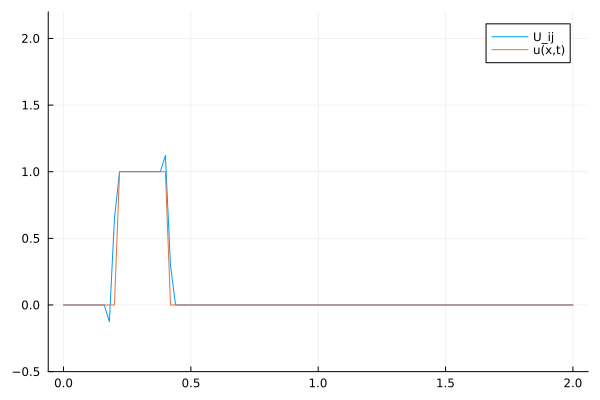
\includegraphics{Trabalho_final_AN_files/gifs/onda2-1}} &
%         \adjustbox{max width=\dimexpr\textwidth/3\relax, max height=\dimexpr\textheight/5\relax}{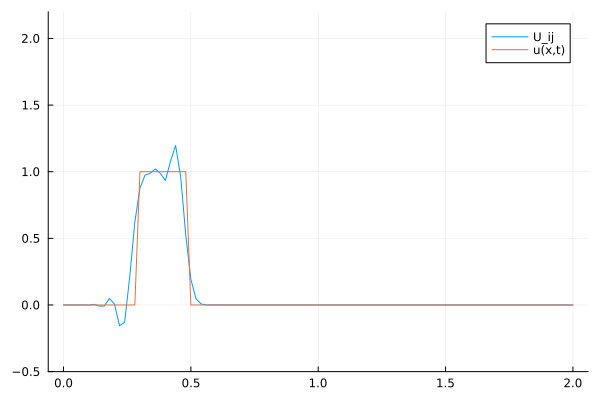
\includegraphics{Trabalho_final_AN_files/gifs/onda2-10}} &
%         \adjustbox{max width=\dimexpr\textwidth/3\relax, max height=\dimexpr\textheight/5\relax}{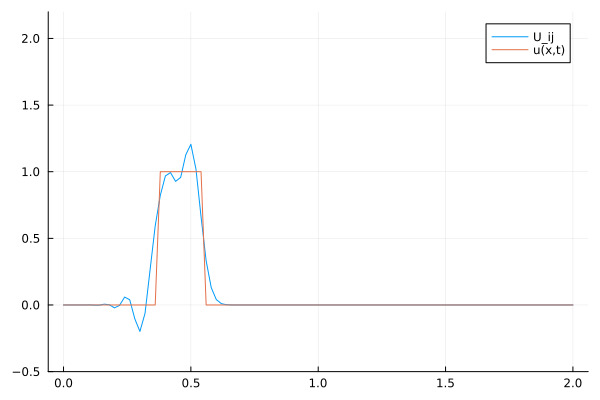
\includegraphics{Trabalho_final_AN_files/gifs/onda2-20}} \\

%         % --- Linha 2 ---
%         \adjustbox{max width=\dimexpr\textwidth/3\relax, max height=\dimexpr\textheight/5\relax}{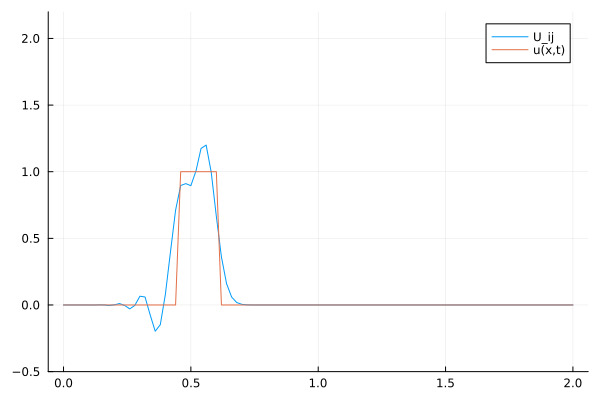
\includegraphics{Trabalho_final_AN_files/gifs/onda2-30}} &
%         \adjustbox{max width=\dimexpr\textwidth/3\relax, max height=\dimexpr\textheight/5\relax}{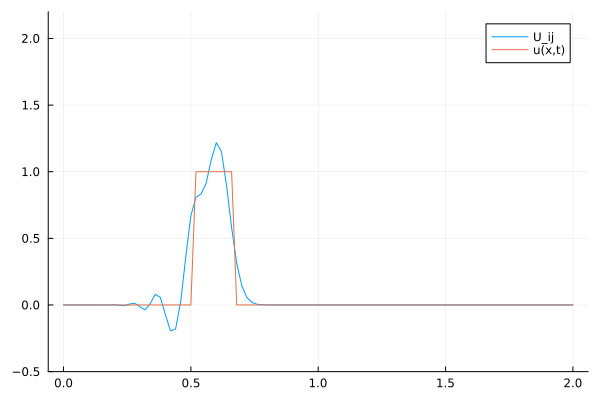
\includegraphics{Trabalho_final_AN_files/gifs/onda2-40}} &
%         \adjustbox{max width=\dimexpr\textwidth/3\relax, max height=\dimexpr\textheight/5\relax}{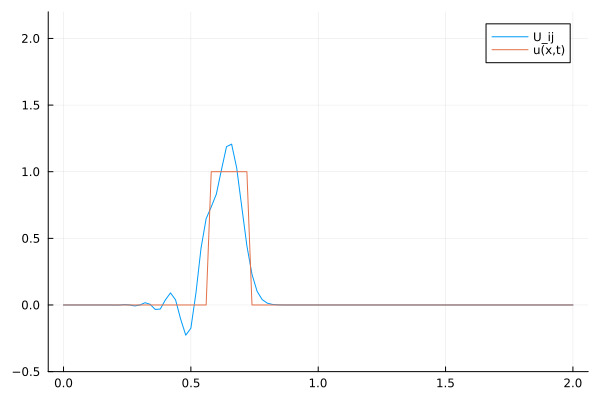
\includegraphics{Trabalho_final_AN_files/gifs/onda2-50}} \\

%         % --- Linha 3 ---
%         \adjustbox{max width=\dimexpr\textwidth/3\relax, max height=\dimexpr\textheight/5\relax}{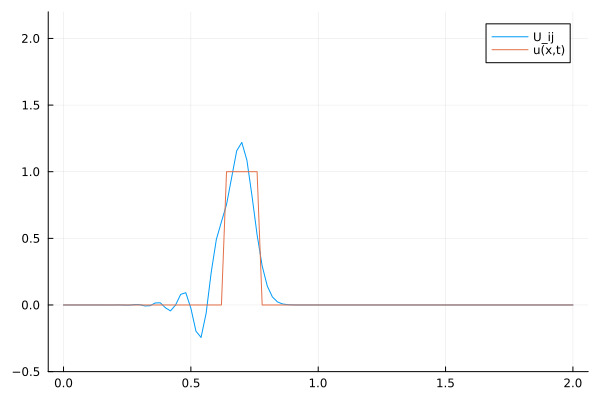
\includegraphics{Trabalho_final_AN_files/gifs/onda2-60}} &
%         \adjustbox{max width=\dimexpr\textwidth/3\relax, max height=\dimexpr\textheight/5\relax}{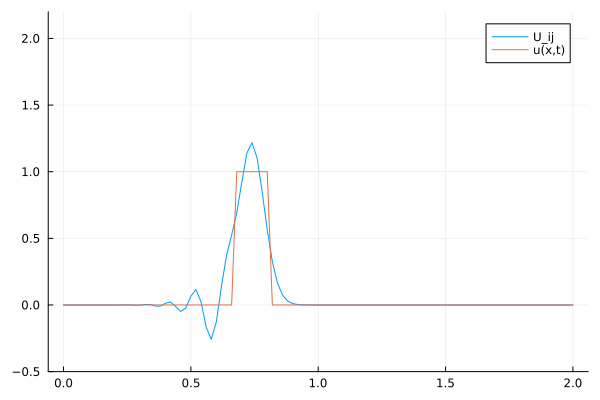
\includegraphics{Trabalho_final_AN_files/gifs/onda2-70}} &
%         \adjustbox{max width=\dimexpr\textwidth/3\relax, max height=\dimexpr\textheight/5\relax}{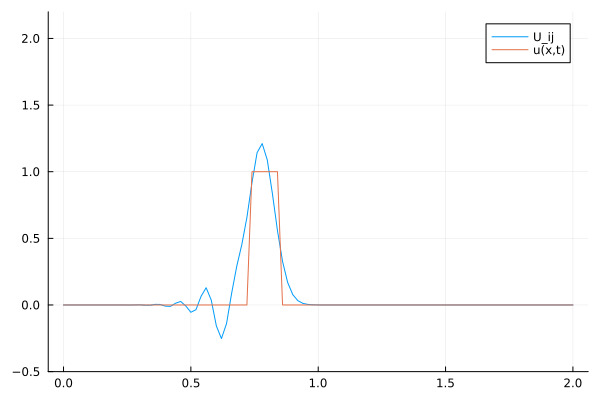
\includegraphics{Trabalho_final_AN_files/gifs/onda2-80}} \\
        
%         % --- Linha 4 --- 
        
%         % Se precisar de 15 imagens, você teria que usar 5 ondas (n=1 a 5) e os 15 frames
%         % Os frames seriam: 0, 15, 30, 45, 60, 75, 90, 105, 120, 135, 150, 165, 180, 195, 210, 225

%         % Para ter *exatamente* 15 imagens (5x3), precisamos de 15 frames.
%         % Os frames solicitados são 0, 15, ..., 225 (16 frames). 
%         % Adaptei para 15 frames: 0, 15, ..., 210, utilizando as primeiras 5 ondas. 
%         % Para incluir o frame 225, você precisaria de um grid 6x3 ou 5x4.
        
%         % Se quiser usar o frame 225, basta adicionar mais uma linha ao \begin{tabular}:
%         % --- Linha 6 (Opcional - se o grid fosse 6x3) ---
%         % \adjustbox{max width=\dimexpr\textwidth/3\relax, max height=\dimexpr\textheight/5\relax}{\includegraphics{Trabalho_final_AN_files/gifs/onda6-225}} & & \\
        
%     \end{tabular}
% \end{center}
        
 
    Observamos uma suavização ao longo do tempo, uns spikes de erros
numéricos, e um efeito de aumento de amplitude da onda.

    \hypertarget{esquema-impluxedcito-de-primeira-ordem}{%
\paragraph{Esquema implícito de primeira
ordem}}
 

    \[U_{i,j} = (1+\nu a)U_{i,j+1} - \nu aU_{i-1,j+1}\]

    \begin{tcolorbox}[breakable, size=fbox, boxrule=1pt, pad at break*=1mm,colback=cellbackground, colframe=cellborder]
\prompt{In}{incolor}{ }{\boxspacing}
\begin{Verbatim}[commandchars=\\\{\}]
\PY{c}{\PYZsh{} Implicito Primeira Ordem}
\PY{n}{h}\PY{+w}{ }\PY{o}{=}\PY{+w}{ }\PY{l+m+mf}{0.02}
\PY{n}{k}\PY{+w}{ }\PY{o}{=}\PY{+w}{ }\PY{l+m+mf}{0.01}

\PY{n}{T}\PY{+w}{ }\PY{o}{=}\PY{+w}{ }\PY{l+m+mi}{100}

\PY{n}{domain}\PY{+w}{ }\PY{o}{=}\PY{+w}{ }\PY{l+m+mi}{0}\PY{o}{:}\PY{n}{h}\PY{o}{:}\PY{l+m+mi}{2}

\PY{n}{U0}\PY{+w}{ }\PY{o}{=}\PY{+w}{  }\PY{n}{u}\PY{o}{.}\PY{p}{(}\PY{n}{domain}\PY{p}{)}\PY{p}{;}


\PY{n}{U}\PY{+w}{ }\PY{o}{=}\PY{+w}{ }\PY{p}{[}\PY{n}{U0}\PY{p}{]}
\PY{n}{ν}\PY{+w}{ }\PY{o}{=}\PY{+w}{ }\PY{n}{k}\PY{o}{/}\PY{n}{h}

\PY{n}{M}\PY{+w}{ }\PY{o}{=}\PY{+w}{ }\PY{n}{length}\PY{p}{(}\PY{n}{U0}\PY{p}{)}

\PY{k}{for}\PY{+w}{ }\PY{n}{j}\PY{o}{=}\PY{l+m+mi}{1}\PY{o}{:}\PY{n}{T}
\PY{+w}{  }\PY{n}{Uj}\PY{+w}{ }\PY{o}{=}\PY{+w}{ }\PY{n}{U}\PY{p}{[}\PY{n}{j}\PY{p}{]}
\PY{+w}{  }\PY{n}{diag}\PY{+w}{ }\PY{o}{=}\PY{+w}{ }\PY{n}{ones}\PY{p}{(}\PY{n}{M}\PY{p}{)}
\PY{+w}{  }\PY{n}{subdiag}\PY{+w}{ }\PY{o}{=}\PY{+w}{ }\PY{n}{zeros}\PY{p}{(}\PY{n}{M}\PY{o}{\PYZhy{}}\PY{l+m+mi}{1}\PY{p}{)}
\PY{+w}{  }\PY{k}{for}\PY{+w}{ }\PY{n}{i}\PY{o}{=}\PY{l+m+mi}{1}\PY{o}{:}\PY{n}{M}\PY{o}{\PYZhy{}}\PY{l+m+mi}{1}
\PY{+w}{    }\PY{n}{xi}\PY{+w}{ }\PY{o}{=}\PY{+w}{ }\PY{p}{(}\PY{n}{i}\PY{o}{+}\PY{l+m+mi}{1}\PY{p}{)}\PY{o}{*}\PY{n}{h}
\PY{+w}{    }\PY{n}{tj}\PY{+w}{ }\PY{o}{=}\PY{+w}{ }\PY{n}{j}\PY{o}{*}\PY{n}{k}
\PY{+w}{    }\PY{n}{va}\PY{+w}{ }\PY{o}{=}\PY{+w}{ }\PY{n}{ν}\PY{o}{*}\PY{n}{a}\PY{p}{(}\PY{n}{xi}\PY{p}{,}\PY{n}{tj}\PY{p}{)}
\PY{+w}{    }\PY{n}{diag}\PY{p}{[}\PY{n}{i}\PY{o}{+}\PY{l+m+mi}{1}\PY{p}{]}\PY{+w}{ }\PY{o}{=}\PY{+w}{ }\PY{l+m+mi}{1}\PY{+w}{ }\PY{o}{+}\PY{+w}{ }\PY{n}{va}
\PY{+w}{    }\PY{n}{subdiag}\PY{p}{[}\PY{n}{i}\PY{p}{]}\PY{+w}{ }\PY{o}{=}\PY{+w}{ }\PY{o}{\PYZhy{}}\PY{n}{va}
\PY{+w}{  }\PY{k}{end}
\PY{+w}{  }\PY{n}{A}\PY{+w}{ }\PY{o}{=}\PY{+w}{ }\PY{n}{Tridiagonal}\PY{p}{(}\PY{n}{subdiag}\PY{p}{,}\PY{+w}{ }\PY{n}{diag}\PY{p}{,}\PY{+w}{ }\PY{n}{zeros}\PY{p}{(}\PY{n}{M}\PY{o}{\PYZhy{}}\PY{l+m+mi}{1}\PY{p}{)}\PY{p}{)}
\PY{+w}{  }\PY{n}{Ujp1}\PY{+w}{ }\PY{o}{=}\PY{+w}{ }\PY{n}{A}\PY{o}{\PYZbs{}}\PY{n}{Uj}
\PY{+w}{  }\PY{n}{push!}\PY{p}{(}\PY{n}{U}\PY{p}{,}\PY{+w}{ }\PY{n}{Ujp1}\PY{p}{)}
\PY{k}{end}
\end{Verbatim}
\end{tcolorbox}

    \begin{tcolorbox}[breakable, size=fbox, boxrule=1pt, pad at break*=1mm,colback=cellbackground, colframe=cellborder]
\prompt{In}{incolor}{ }{\boxspacing}
\begin{Verbatim}[commandchars=\\\{\}]
\PY{n}{graficos}\PY{+w}{ }\PY{o}{=}\PY{+w}{ }\PY{p}{[}\PY{p}{]}
\PY{k}{for}\PY{+w}{ }\PY{n}{t}\PY{o}{=}\PY{p}{[}\PY{l+m+mi}{1}\PY{p}{,}\PY{l+m+mi}{11}\PY{p}{,}\PY{l+m+mi}{51}\PY{p}{,}\PY{l+m+mi}{101}\PY{+w}{ }\PY{p}{]}
\PY{+w}{  }\PY{n}{tt}\PY{+w}{ }\PY{o}{=}\PY{+w}{ }\PY{p}{(}\PY{n}{t}\PY{o}{\PYZhy{}}\PY{l+m+mi}{1}\PY{p}{)}\PY{o}{*}\PY{n}{k}
\PY{+w}{  }\PY{n}{p}\PY{+w}{ }\PY{o}{=}\PY{+w}{ }\PY{n}{plot}\PY{p}{(}\PY{n}{domain}\PY{p}{,}\PY{+w}{ }\PY{n}{U}\PY{p}{[}\PY{n}{t}\PY{p}{]}\PY{p}{,}\PY{+w}{ }\PY{n}{ylim}\PY{o}{=}\PY{p}{(}\PY{o}{\PYZhy{}}\PY{l+m+mf}{0.5}\PY{p}{,}\PY{l+m+mf}{1.2}\PY{p}{)}\PY{p}{,}\PY{+w}{ }\PY{n}{label}\PY{o}{=}\PY{l+s}{\PYZdq{}}\PY{l+s}{U\PYZus{}ij}\PY{l+s}{\PYZdq{}}\PY{p}{,}\PY{+w}{ }\PY{n}{title}\PY{o}{=}\PY{l+s}{\PYZdq{}}\PY{l+s}{t=}\PY{l+s+si}{\PYZdl{}tt}\PY{l+s}{\PYZdq{}}\PY{p}{)}
\PY{+w}{  }\PY{n}{solu}\PY{p}{(}\PY{n}{z}\PY{p}{)}\PY{+w}{ }\PY{o}{=}\PY{+w}{ }\PY{n}{z}\PY{o}{\PYZhy{}}\PY{+w}{ }\PY{n}{tt}\PY{o}{/}\PY{p}{(}\PY{l+m+mi}{1}\PY{o}{+}\PY{n}{z}\PY{o}{\PYZca{}}\PY{l+m+mi}{2}\PY{p}{)}
\PY{+w}{  }\PY{n}{plot!}\PY{p}{(}\PY{n}{p}\PY{p}{,}\PY{+w}{ }\PY{n}{domain}\PY{p}{,}\PY{+w}{ }\PY{n}{u}\PY{o}{.}\PY{p}{(}\PY{n}{solu}\PY{o}{.}\PY{p}{(}\PY{n}{domain}\PY{p}{)}\PY{p}{)}\PY{p}{,}\PY{+w}{ }\PY{n}{label}\PY{o}{=}\PY{l+s}{\PYZdq{}}\PY{l+s}{u(x,t)}\PY{l+s}{\PYZdq{}}\PY{p}{)}
\PY{+w}{  }\PY{n}{push!}\PY{p}{(}\PY{n}{graficos}\PY{p}{,}\PY{+w}{ }\PY{n}{p}\PY{p}{)}
\PY{k}{end}
\PY{n}{plot}\PY{p}{(}\PY{n}{graficos}\PY{o}{...}\PY{p}{;}\PY{+w}{ }\PY{n}{layout}\PY{o}{=}\PY{n+nd}{@layout}\PY{p}{(}\PY{p}{[}\PY{n}{°}\PY{+w}{ }\PY{n}{°}\PY{p}{;}\PY{+w}{ }\PY{n}{°}\PY{+w}{ }\PY{n}{°}\PY{p}{]}\PY{p}{)}\PY{p}{,}\PY{+w}{ }\PY{n}{size}\PY{o}{=}\PY{p}{(}\PY{l+m+mi}{1200}\PY{p}{,}\PY{l+m+mi}{600}\PY{p}{)}\PY{p}{)}
\end{Verbatim}
\end{tcolorbox}
 
            
\prompt{Out}{outcolor}{ }{}
    
    \begin{center}
    \adjustimage{max size={0.9\linewidth}{0.9\paperheight}}{Trabalho_final_AN_files/Trabalho_final_AN_39_0.pdf}
    \end{center}
    { \hspace*{\fill} \\}
      



% Para centralizar a tabela na página
% \begin{center}
%     % Definimos um array de 3 colunas, todas centralizadas (c)
%     % A largura da coluna será automaticamente calculada.
%     % A largura total da tabela é ajustada para \textwidth (largura do texto)
%     % Ajustamos o espaçamento entre as colunas (colsep) e linhas (rowsep) para ficar mais apertado, se necessário.
%     \setlength{\tabcolsep}{1pt} % Espaçamento horizontal entre colunas
%     \renewcommand{\arraystretch}{0.5} % Espaçamento vertical entre linhas
    
%     \begin{tabular}{ccc} % 3 colunas

%         % --- Linha 1 ---
%         % As imagens são ajustadas para ter 1/3 da largura do texto menos o espaçamento.
%         % Você pode ajustar a escala (\scalebox) se for mais conveniente.
%         \adjustbox{max width=\dimexpr\textwidth/3\relax, max height=\dimexpr\textheight/5\relax}{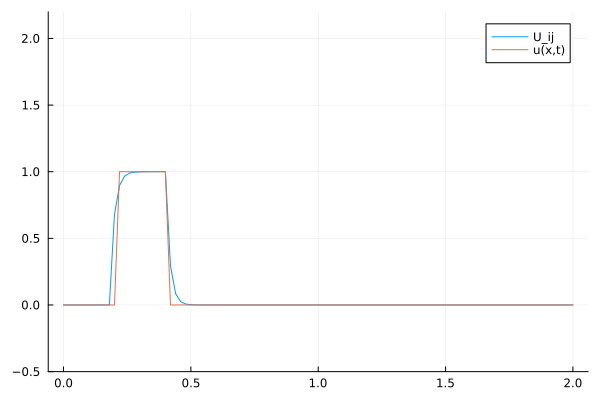
\includegraphics{Trabalho_final_AN_files/gifs/onda3-1}} &
%         \adjustbox{max width=\dimexpr\textwidth/3\relax, max height=\dimexpr\textheight/5\relax}{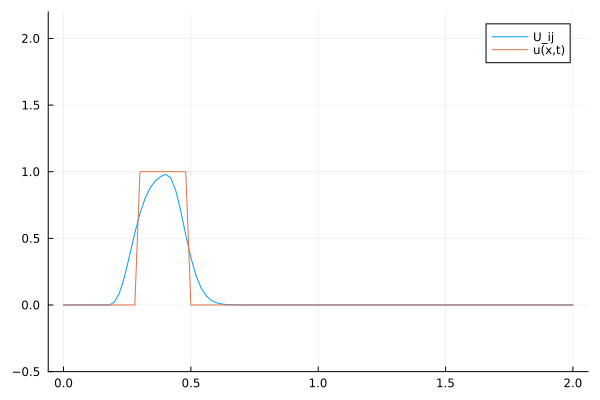
\includegraphics{Trabalho_final_AN_files/gifs/onda3-10}} &
%         \adjustbox{max width=\dimexpr\textwidth/3\relax, max height=\dimexpr\textheight/5\relax}{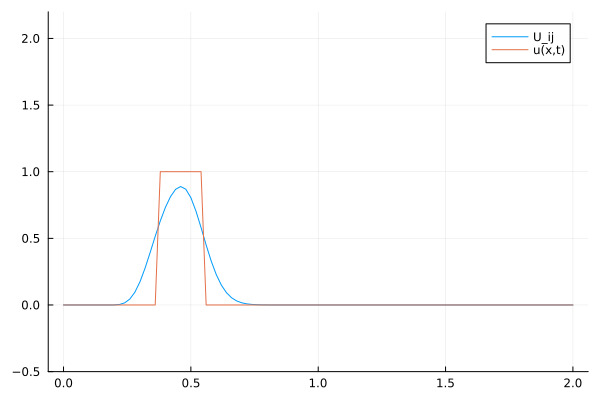
\includegraphics{Trabalho_final_AN_files/gifs/onda3-20}} \\

%         % --- Linha 2 ---
%         \adjustbox{max width=\dimexpr\textwidth/3\relax, max height=\dimexpr\textheight/5\relax}{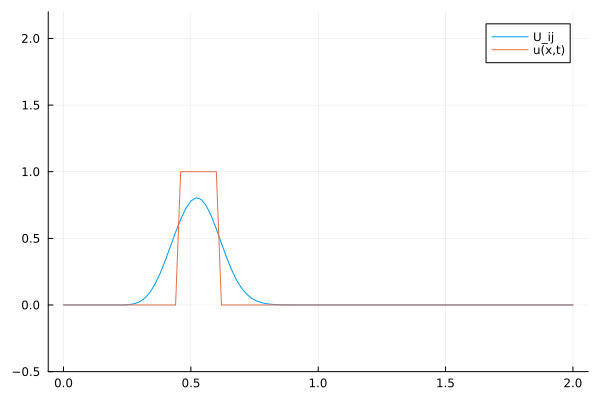
\includegraphics{Trabalho_final_AN_files/gifs/onda3-30}} &
%         \adjustbox{max width=\dimexpr\textwidth/3\relax, max height=\dimexpr\textheight/5\relax}{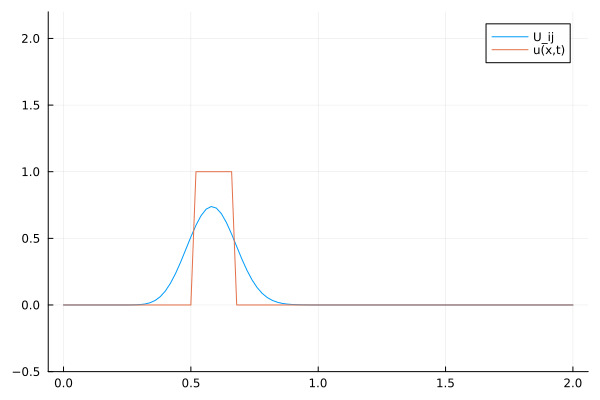
\includegraphics{Trabalho_final_AN_files/gifs/onda3-40}} &
%         \adjustbox{max width=\dimexpr\textwidth/3\relax, max height=\dimexpr\textheight/5\relax}{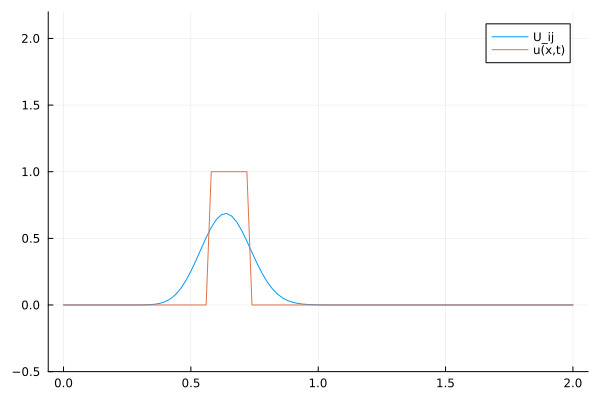
\includegraphics{Trabalho_final_AN_files/gifs/onda3-50}} \\

%         % --- Linha 3 ---
%         \adjustbox{max width=\dimexpr\textwidth/3\relax, max height=\dimexpr\textheight/5\relax}{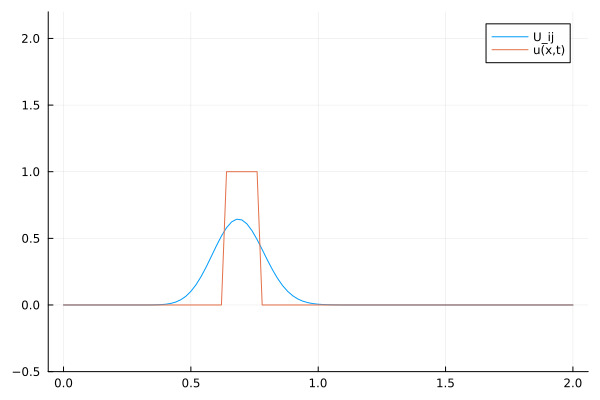
\includegraphics{Trabalho_final_AN_files/gifs/onda3-60}} &
%         \adjustbox{max width=\dimexpr\textwidth/3\relax, max height=\dimexpr\textheight/5\relax}{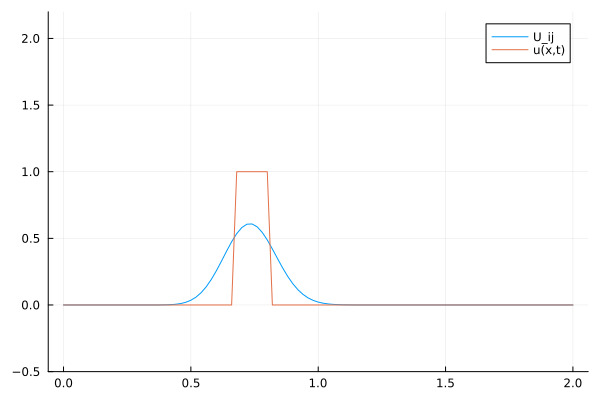
\includegraphics{Trabalho_final_AN_files/gifs/onda3-70}} &
%         \adjustbox{max width=\dimexpr\textwidth/3\relax, max height=\dimexpr\textheight/5\relax}{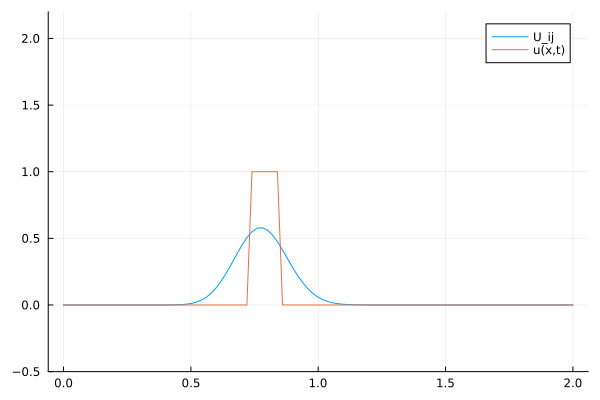
\includegraphics{Trabalho_final_AN_files/gifs/onda3-80}} \\
        
%         % --- Linha 4 --- 
        
%         % Se precisar de 15 imagens, você teria que usar 5 ondas (n=1 a 5) e os 15 frames
%         % Os frames seriam: 0, 15, 30, 45, 60, 75, 90, 105, 120, 135, 150, 165, 180, 195, 210, 225

%         % Para ter *exatamente* 15 imagens (5x3), precisamos de 15 frames.
%         % Os frames solicitados são 0, 15, ..., 225 (16 frames). 
%         % Adaptei para 15 frames: 0, 15, ..., 210, utilizando as primeiras 5 ondas. 
%         % Para incluir o frame 225, você precisaria de um grid 6x3 ou 5x4.
        
%         % Se quiser usar o frame 225, basta adicionar mais uma linha ao \begin{tabular}:
%         % --- Linha 6 (Opcional - se o grid fosse 6x3) ---
%         % \adjustbox{max width=\dimexpr\textwidth/3\relax, max height=\dimexpr\textheight/5\relax}{\includegraphics{Trabalho_final_AN_files/gifs/onda6-225}} & & \\
        
%     \end{tabular}
% \end{center}
        

        
    Temos uma suavização da descontinuidade bem como um efeito de
dissipação.

    \hypertarget{muxe9todo-box}{%
\paragraph{Método Box}}

    \begin{figure}
\centering
\caption{image.png}
\end{figure}

    \[U_{i+1,j+1} + \frac{1-\nu a}{1+\nu a}U_{i,j+1} = U_{i,j} + \frac{1-\nu a}{1+\nu a}U_{i+1,j}\]

    \begin{tcolorbox}[breakable, size=fbox, boxrule=1pt, pad at break*=1mm,colback=cellbackground, colframe=cellborder]
\prompt{In}{incolor}{ }{\boxspacing}
\begin{Verbatim}[commandchars=\\\{\}]
\PY{+w}{ }\PY{c}{\PYZsh{} Método Box}
\PY{n}{h}\PY{+w}{ }\PY{o}{=}\PY{+w}{ }\PY{l+m+mf}{0.02}
\PY{n}{k}\PY{+w}{ }\PY{o}{=}\PY{+w}{ }\PY{l+m+mf}{0.01}

\PY{n}{T}\PY{+w}{ }\PY{o}{=}\PY{+w}{ }\PY{l+m+mi}{100}

\PY{n}{domain}\PY{+w}{ }\PY{o}{=}\PY{+w}{ }\PY{l+m+mi}{0}\PY{o}{:}\PY{n}{h}\PY{o}{:}\PY{l+m+mi}{2}

\PY{n}{U0}\PY{+w}{ }\PY{o}{=}\PY{+w}{  }\PY{n}{u}\PY{o}{.}\PY{p}{(}\PY{n}{domain}\PY{p}{)}\PY{p}{;}


\PY{n}{U}\PY{+w}{ }\PY{o}{=}\PY{+w}{ }\PY{p}{[}\PY{n}{U0}\PY{p}{]}
\PY{n}{ν}\PY{+w}{ }\PY{o}{=}\PY{+w}{ }\PY{n}{k}\PY{o}{/}\PY{n}{h}

\PY{n}{M}\PY{+w}{ }\PY{o}{=}\PY{+w}{ }\PY{n}{length}\PY{p}{(}\PY{n}{U0}\PY{p}{)}


\PY{k}{for}\PY{+w}{ }\PY{n}{j}\PY{o}{=}\PY{l+m+mi}{1}\PY{o}{:}\PY{n}{T}
\PY{+w}{  }\PY{n}{Uj}\PY{+w}{ }\PY{o}{=}\PY{+w}{ }\PY{n}{U}\PY{p}{[}\PY{n}{j}\PY{p}{]}

\PY{+w}{  }\PY{n}{Ujp1}\PY{+w}{ }\PY{o}{=}\PY{+w}{ }\PY{n}{zeros}\PY{p}{(}\PY{n}{M}\PY{p}{)}
\PY{+w}{  }\PY{n}{diagA}\PY{+w}{ }\PY{o}{=}\PY{+w}{ }\PY{n}{ones}\PY{p}{(}\PY{n}{M}\PY{p}{)}
\PY{+w}{  }\PY{n}{subdiagB}\PY{+w}{ }\PY{o}{=}\PY{+w}{ }\PY{n}{zeros}\PY{p}{(}\PY{n}{M}\PY{p}{)}
\PY{+w}{  }\PY{k}{for}\PY{+w}{ }\PY{n}{i}\PY{o}{=}\PY{l+m+mi}{1}\PY{o}{:}\PY{n}{M}\PY{o}{\PYZhy{}}\PY{l+m+mi}{1}
\PY{+w}{    }\PY{n}{xi}\PY{+w}{ }\PY{o}{=}\PY{+w}{ }\PY{p}{(}\PY{n}{i}\PY{o}{\PYZhy{}}\PY{l+m+mi}{1}\PY{p}{)}\PY{o}{*}\PY{n}{h}\PY{+w}{  }\PY{c}{\PYZsh{} Correção: índice começa em 0}
\PY{+w}{    }\PY{n}{tj}\PY{+w}{ }\PY{o}{=}\PY{+w}{ }\PY{p}{(}\PY{n}{j}\PY{o}{\PYZhy{}}\PY{l+m+mi}{1}\PY{p}{)}\PY{o}{*}\PY{n}{k}
\PY{+w}{    }\PY{n}{va}\PY{+w}{ }\PY{o}{=}\PY{+w}{ }\PY{n}{ν}\PY{o}{*}\PY{n}{a}\PY{p}{(}\PY{n}{xi}\PY{p}{,}\PY{n}{tj}\PY{p}{)}
\PY{+w}{    }\PY{n}{λ}\PY{+w}{ }\PY{o}{=}\PY{+w}{ }\PY{p}{(}\PY{l+m+mi}{1}\PY{+w}{ }\PY{o}{\PYZhy{}}\PY{+w}{ }\PY{n}{va}\PY{p}{)}\PY{o}{/}\PY{p}{(}\PY{l+m+mi}{1}\PY{+w}{ }\PY{o}{+}\PY{+w}{ }\PY{n}{va}\PY{p}{)}
\PY{+w}{    }\PY{k}{if}\PY{+w}{ }\PY{n}{i}\PY{+w}{ }\PY{o}{==}\PY{+w}{ }\PY{l+m+mi}{1}
\PY{+w}{    }\PY{c}{\PYZsh{} Para i=1: U\PYZus{}\PYZob{}1,j+1\PYZcb{} = 0 (condição de contorno)}
\PY{+w}{    }\PY{c}{\PYZsh{} Equação: U\PYZus{}\PYZob{}2,j+1\PYZcb{} + λ * 0 = U\PYZus{}\PYZob{}1,j\PYZcb{} + λ * U\PYZus{}\PYZob{}2,j\PYZcb{}}
\PY{+w}{        }\PY{n}{Ujp1}\PY{p}{[}\PY{l+m+mi}{2}\PY{p}{]}\PY{+w}{ }\PY{o}{=}\PY{+w}{ }\PY{n}{Uj}\PY{p}{[}\PY{l+m+mi}{1}\PY{p}{]}\PY{+w}{ }\PY{o}{+}\PY{+w}{ }\PY{n}{λ}\PY{+w}{ }\PY{o}{*}\PY{+w}{ }\PY{n}{Uj}\PY{p}{[}\PY{l+m+mi}{2}\PY{p}{]}
\PY{+w}{    }\PY{k}{else}
\PY{+w}{        }\PY{c}{\PYZsh{} Para i\PYZgt{}1: U\PYZus{}\PYZob{}i+1,j+1\PYZcb{} + λ * U\PYZus{}\PYZob{}i,j+1\PYZcb{} = U\PYZus{}\PYZob{}i,j\PYZcb{} + λ * U\PYZus{}\PYZob{}i+1,j\PYZcb{}}
\PY{+w}{        }\PY{c}{\PYZsh{} Isolando U\PYZus{}\PYZob{}i+1,j+1\PYZcb{}:}
\PY{+w}{        }\PY{n}{Ujp1}\PY{p}{[}\PY{n}{i}\PY{o}{+}\PY{l+m+mi}{1}\PY{p}{]}\PY{+w}{ }\PY{o}{=}\PY{+w}{ }\PY{n}{Uj}\PY{p}{[}\PY{n}{i}\PY{p}{]}\PY{+w}{ }\PY{o}{+}\PY{+w}{ }\PY{n}{λ}\PY{+w}{ }\PY{o}{*}\PY{+w}{ }\PY{n}{Uj}\PY{p}{[}\PY{n}{i}\PY{o}{+}\PY{l+m+mi}{1}\PY{p}{]}\PY{+w}{ }\PY{o}{\PYZhy{}}\PY{+w}{ }\PY{n}{λ}\PY{+w}{ }\PY{o}{*}\PY{+w}{ }\PY{n}{Ujp1}\PY{p}{[}\PY{n}{i}\PY{p}{]}
\PY{+w}{    }\PY{k}{end}
\PY{+w}{  }\PY{k}{end}
\PY{+w}{  }\PY{n}{push!}\PY{p}{(}\PY{n}{U}\PY{p}{,}\PY{n}{Ujp1}\PY{p}{)}
\PY{k}{end}
\end{Verbatim}
\end{tcolorbox}

    \begin{tcolorbox}[breakable, size=fbox, boxrule=1pt, pad at break*=1mm,colback=cellbackground, colframe=cellborder]
\prompt{In}{incolor}{ }{\boxspacing}
\begin{Verbatim}[commandchars=\\\{\}]
\PY{n}{graficos}\PY{+w}{ }\PY{o}{=}\PY{+w}{ }\PY{p}{[}\PY{p}{]}
\PY{k}{for}\PY{+w}{ }\PY{n}{t}\PY{o}{=}\PY{p}{[}\PY{l+m+mi}{1}\PY{p}{,}\PY{l+m+mi}{11}\PY{p}{,}\PY{l+m+mi}{51}\PY{p}{,}\PY{l+m+mi}{101}\PY{+w}{ }\PY{p}{]}
\PY{+w}{  }\PY{n}{tt}\PY{+w}{ }\PY{o}{=}\PY{+w}{ }\PY{p}{(}\PY{n}{t}\PY{o}{\PYZhy{}}\PY{l+m+mi}{1}\PY{p}{)}\PY{o}{*}\PY{n}{k}
\PY{+w}{  }\PY{n}{p}\PY{+w}{ }\PY{o}{=}\PY{+w}{ }\PY{n}{plot}\PY{p}{(}\PY{n}{domain}\PY{p}{,}\PY{+w}{ }\PY{n}{U}\PY{p}{[}\PY{n}{t}\PY{p}{]}\PY{p}{,}\PY{+w}{ }\PY{n}{ylim}\PY{o}{=}\PY{p}{(}\PY{o}{\PYZhy{}}\PY{l+m+mf}{0.5}\PY{p}{,}\PY{l+m+mf}{1.2}\PY{p}{)}\PY{p}{,}\PY{+w}{ }\PY{n}{label}\PY{o}{=}\PY{l+s}{\PYZdq{}}\PY{l+s}{U\PYZus{}ij}\PY{l+s}{\PYZdq{}}\PY{p}{,}\PY{+w}{ }\PY{n}{title}\PY{o}{=}\PY{l+s}{\PYZdq{}}\PY{l+s}{t=}\PY{l+s+si}{\PYZdl{}tt}\PY{l+s}{\PYZdq{}}\PY{p}{)}
\PY{+w}{  }\PY{n}{solu}\PY{p}{(}\PY{n}{z}\PY{p}{)}\PY{+w}{ }\PY{o}{=}\PY{+w}{ }\PY{n}{z}\PY{o}{\PYZhy{}}\PY{+w}{ }\PY{n}{tt}\PY{o}{/}\PY{p}{(}\PY{l+m+mi}{1}\PY{o}{+}\PY{n}{z}\PY{o}{\PYZca{}}\PY{l+m+mi}{2}\PY{p}{)}
\PY{+w}{  }\PY{n}{plot!}\PY{p}{(}\PY{n}{p}\PY{p}{,}\PY{+w}{ }\PY{n}{domain}\PY{p}{,}\PY{+w}{ }\PY{n}{u}\PY{o}{.}\PY{p}{(}\PY{n}{solu}\PY{o}{.}\PY{p}{(}\PY{n}{domain}\PY{p}{)}\PY{p}{)}\PY{p}{,}\PY{+w}{ }\PY{n}{label}\PY{o}{=}\PY{l+s}{\PYZdq{}}\PY{l+s}{u(x,t)}\PY{l+s}{\PYZdq{}}\PY{p}{)}
\PY{+w}{  }\PY{n}{push!}\PY{p}{(}\PY{n}{graficos}\PY{p}{,}\PY{+w}{ }\PY{n}{p}\PY{p}{)}
\PY{k}{end}
\PY{n}{plot}\PY{p}{(}\PY{n}{graficos}\PY{o}{...}\PY{p}{;}\PY{+w}{ }\PY{n}{layout}\PY{o}{=}\PY{n+nd}{@layout}\PY{p}{(}\PY{p}{[}\PY{n}{°}\PY{+w}{ }\PY{n}{°}\PY{p}{;}\PY{+w}{ }\PY{n}{°}\PY{+w}{ }\PY{n}{°}\PY{p}{]}\PY{p}{)}\PY{p}{,}\PY{+w}{ }\PY{n}{size}\PY{o}{=}\PY{p}{(}\PY{l+m+mi}{1200}\PY{p}{,}\PY{l+m+mi}{600}\PY{p}{)}\PY{p}{)}
\end{Verbatim}
\end{tcolorbox}
 
            
\prompt{Out}{outcolor}{ }{}
    
    \begin{center}
    \adjustimage{max size={0.9\linewidth}{0.9\paperheight}}{Trabalho_final_AN_files/Trabalho_final_AN_46_0.pdf}
    \end{center}
    { \hspace*{\fill} \\}
    
 % Metodo Box



% Para centralizar a tabela na página
% \begin{center}
%     % Definimos um array de 3 colunas, todas centralizadas (c)
%     % A largura da coluna será automaticamente calculada.
%     % A largura total da tabela é ajustada para \textwidth (largura do texto)
%     % Ajustamos o espaçamento entre as colunas (colsep) e linhas (rowsep) para ficar mais apertado, se necessário.
%     \setlength{\tabcolsep}{1pt} % Espaçamento horizontal entre colunas
%     \renewcommand{\arraystretch}{0.5} % Espaçamento vertical entre linhas
    
%     \begin{tabular}{ccc} % 3 colunas

%         % --- Linha 1 ---
%         % As imagens são ajustadas para ter 1/3 da largura do texto menos o espaçamento.
%         % Você pode ajustar a escala (\scalebox) se for mais conveniente.
%         \adjustbox{max width=\dimexpr\textwidth/3\relax, max height=\dimexpr\textheight/5\relax}{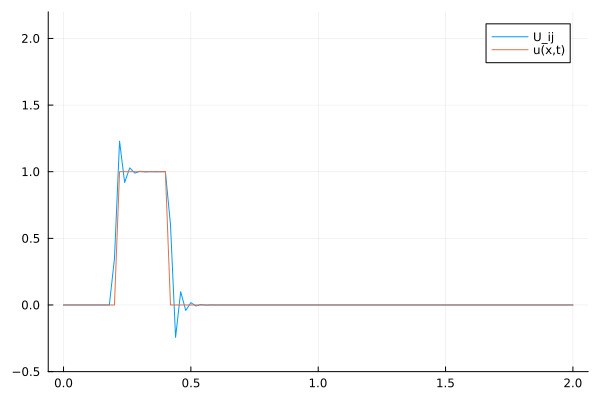
\includegraphics{Trabalho_final_AN_files/gifs/onda4-1}} &
%         \adjustbox{max width=\dimexpr\textwidth/3\relax, max height=\dimexpr\textheight/5\relax}{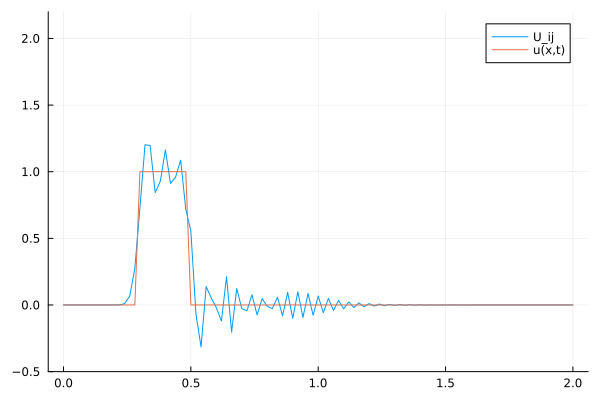
\includegraphics{Trabalho_final_AN_files/gifs/onda4-10}} &
%         \adjustbox{max width=\dimexpr\textwidth/3\relax, max height=\dimexpr\textheight/5\relax}{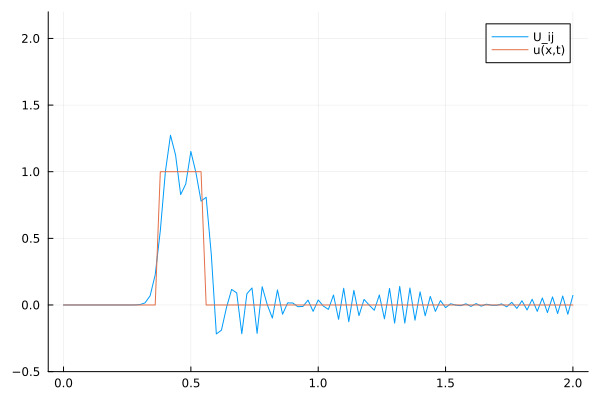
\includegraphics{Trabalho_final_AN_files/gifs/onda4-20}} \\

%         % --- Linha 2 ---
%         \adjustbox{max width=\dimexpr\textwidth/3\relax, max height=\dimexpr\textheight/5\relax}{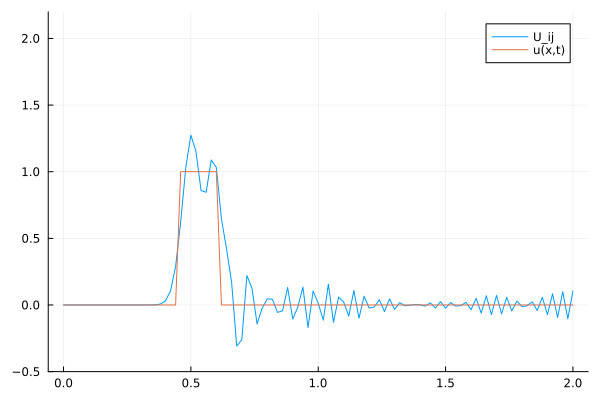
\includegraphics{Trabalho_final_AN_files/gifs/onda4-30}} &
%         \adjustbox{max width=\dimexpr\textwidth/3\relax, max height=\dimexpr\textheight/5\relax}{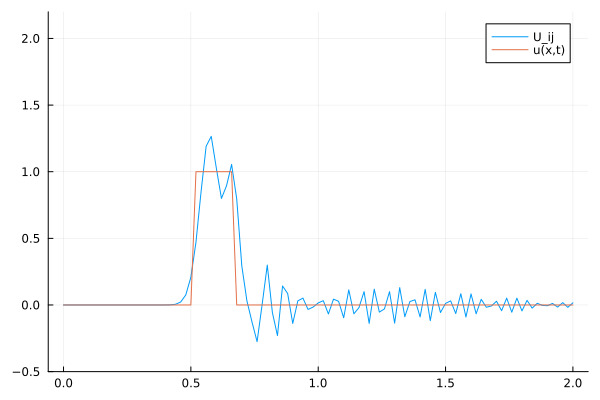
\includegraphics{Trabalho_final_AN_files/gifs/onda4-40}} &
%         \adjustbox{max width=\dimexpr\textwidth/3\relax, max height=\dimexpr\textheight/5\relax}{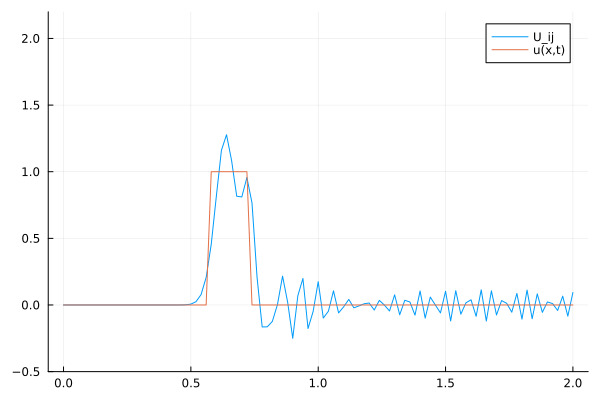
\includegraphics{Trabalho_final_AN_files/gifs/onda4-50}} \\

%         % --- Linha 3 ---
%         \adjustbox{max width=\dimexpr\textwidth/3\relax, max height=\dimexpr\textheight/5\relax}{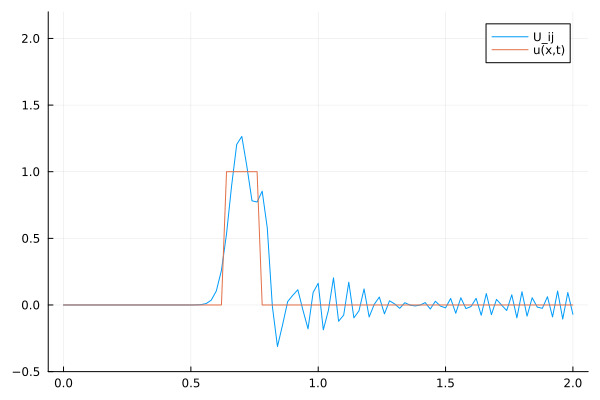
\includegraphics{Trabalho_final_AN_files/gifs/onda4-60}} &
%         \adjustbox{max width=\dimexpr\textwidth/3\relax, max height=\dimexpr\textheight/5\relax}{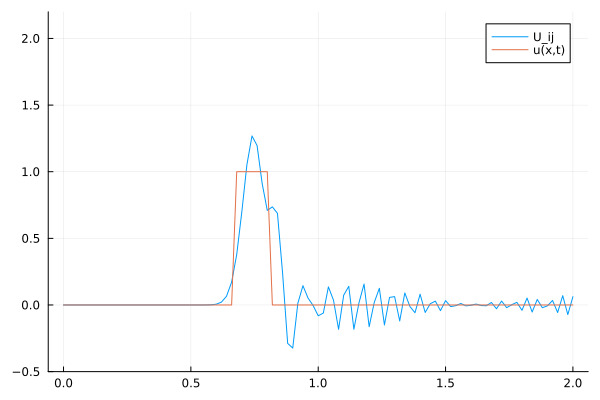
\includegraphics{Trabalho_final_AN_files/gifs/onda4-70}} &
%         \adjustbox{max width=\dimexpr\textwidth/3\relax, max height=\dimexpr\textheight/5\relax}{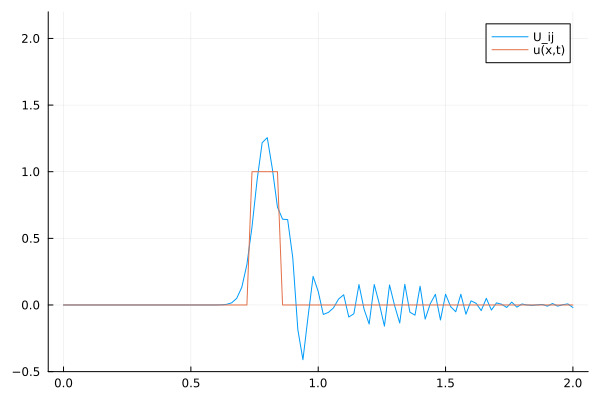
\includegraphics{Trabalho_final_AN_files/gifs/onda4-80}} \\
        
%         % --- Linha 4 --- 
        
%         % Se precisar de 15 imagens, você teria que usar 5 ondas (n=1 a 5) e os 15 frames
%         % Os frames seriam: 0, 15, 30, 45, 60, 75, 90, 105, 120, 135, 150, 165, 180, 195, 210, 225

%         % Para ter *exatamente* 15 imagens (5x3), precisamos de 15 frames.
%         % Os frames solicitados são 0, 15, ..., 225 (16 frames). 
%         % Adaptei para 15 frames: 0, 15, ..., 210, utilizando as primeiras 5 ondas. 
%         % Para incluir o frame 225, você precisaria de um grid 6x3 ou 5x4.
        
%         % Se quiser usar o frame 225, basta adicionar mais uma linha ao \begin{tabular}:
%         % --- Linha 6 (Opcional - se o grid fosse 6x3) ---
%         % \adjustbox{max width=\dimexpr\textwidth/3\relax, max height=\dimexpr\textheight/5\relax}{\includegraphics{Trabalho_final_AN_files/gifs/onda6-225}} & & \\
        
%     \end{tabular}
% \end{center}
        

        
    \hypertarget{muxe9todo-upwind}{%
\paragraph{\texorpdfstring{Método
\emph{upwind}}{Método upwind}}}

    \begin{figure}
\centering
\caption{image.png}
\end{figure}

    \[U_{i,j+1} = U_{i,j} - \frac{a\nu}{2}(U_{i+1,j} - U_{i-1,j}) + \frac{|a|\nu}2(U_{i+1,j}-2U_{i,j}+U_{i-1,j})  \]

    \begin{tcolorbox}[breakable, size=fbox, boxrule=1pt, pad at break*=1mm,colback=cellbackground, colframe=cellborder]
\prompt{In}{incolor}{ }{\boxspacing}
\begin{Verbatim}[commandchars=\\\{\}]
\PY{c}{\PYZsh{} upwind}
\PY{n}{h}\PY{+w}{ }\PY{o}{=}\PY{+w}{ }\PY{l+m+mf}{0.02}
\PY{n}{k}\PY{+w}{ }\PY{o}{=}\PY{+w}{ }\PY{l+m+mf}{0.01}

\PY{n}{T}\PY{+w}{ }\PY{o}{=}\PY{+w}{ }\PY{l+m+mi}{100}

\PY{n}{domain}\PY{+w}{ }\PY{o}{=}\PY{+w}{ }\PY{l+m+mi}{0}\PY{o}{:}\PY{n}{h}\PY{o}{:}\PY{l+m+mi}{2}
\PY{n}{U0}\PY{+w}{ }\PY{o}{=}\PY{+w}{  }\PY{n}{u}\PY{o}{.}\PY{p}{(}\PY{n}{domain}\PY{p}{)}\PY{p}{;}
\PY{n}{U}\PY{+w}{ }\PY{o}{=}\PY{+w}{ }\PY{p}{[}\PY{n}{U0}\PY{p}{]}
\PY{n}{ν}\PY{+w}{ }\PY{o}{=}\PY{+w}{ }\PY{n}{k}\PY{o}{/}\PY{n}{h}

\PY{n}{M}\PY{+w}{ }\PY{o}{=}\PY{+w}{ }\PY{n}{length}\PY{p}{(}\PY{n}{U0}\PY{p}{)}

\PY{k}{for}\PY{+w}{ }\PY{n}{j}\PY{o}{=}\PY{l+m+mi}{1}\PY{o}{:}\PY{n}{T}
\PY{+w}{  }\PY{n}{Uj}\PY{+w}{ }\PY{o}{=}\PY{+w}{ }\PY{n}{U}\PY{p}{[}\PY{n}{j}\PY{p}{]}
\PY{+w}{  }\PY{n}{Ujp1}\PY{+w}{ }\PY{o}{=}\PY{+w}{ }\PY{n}{zeros}\PY{p}{(}\PY{n}{M}\PY{p}{)}

\PY{+w}{  }\PY{n}{subdA}\PY{+w}{ }\PY{o}{=}\PY{+w}{ }\PY{n}{zeros}\PY{p}{(}\PY{n}{M}\PY{o}{\PYZhy{}}\PY{l+m+mi}{1}\PY{p}{)}
\PY{+w}{  }\PY{n}{diagA}\PY{+w}{ }\PY{o}{=}\PY{+w}{ }\PY{n}{ones}\PY{p}{(}\PY{n}{M}\PY{p}{)}
\PY{+w}{  }\PY{n}{supdA}\PY{+w}{ }\PY{o}{=}\PY{+w}{ }\PY{n}{zeros}\PY{p}{(}\PY{n}{M}\PY{o}{\PYZhy{}}\PY{l+m+mi}{1}\PY{p}{)}

\PY{+w}{  }\PY{n}{subdB}\PY{+w}{ }\PY{o}{=}\PY{+w}{ }\PY{n}{zeros}\PY{p}{(}\PY{n}{M}\PY{o}{\PYZhy{}}\PY{l+m+mi}{1}\PY{p}{)}
\PY{+w}{  }\PY{n}{diagB}\PY{+w}{ }\PY{o}{=}\PY{+w}{ }\PY{n}{ones}\PY{p}{(}\PY{n}{M}\PY{p}{)}
\PY{+w}{  }\PY{n}{supdB}\PY{+w}{ }\PY{o}{=}\PY{+w}{ }\PY{n}{zeros}\PY{p}{(}\PY{n}{M}\PY{o}{\PYZhy{}}\PY{l+m+mi}{1}\PY{p}{)}
\PY{+w}{  }\PY{k}{for}\PY{+w}{ }\PY{n}{i}\PY{o}{=}\PY{l+m+mi}{2}\PY{o}{:}\PY{n}{M}\PY{o}{\PYZhy{}}\PY{l+m+mi}{1}
\PY{+w}{    }\PY{n}{xi}\PY{+w}{ }\PY{o}{=}\PY{+w}{ }\PY{n}{i}\PY{o}{*}\PY{n}{h}
\PY{+w}{    }\PY{n}{tj}\PY{+w}{ }\PY{o}{=}\PY{+w}{ }\PY{n}{j}\PY{o}{*}\PY{n}{k}
\PY{+w}{    }\PY{n}{va}\PY{+w}{ }\PY{o}{=}\PY{+w}{ }\PY{n}{ν}\PY{o}{*}\PY{n}{a}\PY{p}{(}\PY{n}{xi}\PY{p}{,}\PY{n}{tj}\PY{p}{)}
\PY{+w}{    }\PY{n}{vap}\PY{+w}{ }\PY{o}{=}\PY{+w}{ }\PY{n}{ν}\PY{o}{*}\PY{n}{abs}\PY{p}{(}\PY{n}{a}\PY{p}{(}\PY{n}{xi}\PY{p}{,}\PY{n}{tj}\PY{p}{)}\PY{p}{)}
\PY{+w}{    }\PY{n}{Ujp1}\PY{p}{[}\PY{n}{i}\PY{p}{]}\PY{+w}{ }\PY{o}{=}\PY{+w}{ }\PY{n}{Uj}\PY{p}{[}\PY{n}{i}\PY{p}{]}\PY{+w}{ }\PY{o}{\PYZhy{}}\PY{+w}{ }\PY{n}{va}\PY{o}{/}\PY{l+m+mi}{2}\PY{o}{*}\PY{p}{(}\PY{n}{Uj}\PY{p}{[}\PY{n}{i}\PY{o}{+}\PY{l+m+mi}{1}\PY{p}{]}\PY{+w}{ }\PY{o}{\PYZhy{}}\PY{+w}{ }\PY{n}{Uj}\PY{p}{[}\PY{n}{i}\PY{o}{\PYZhy{}}\PY{l+m+mi}{1}\PY{p}{]}\PY{p}{)}\PY{+w}{ }\PY{o}{+}\PY{+w}{ }\PY{n}{vap}\PY{o}{/}\PY{l+m+mi}{2}\PY{o}{*}\PY{p}{(}\PY{n}{Uj}\PY{p}{[}\PY{n}{i}\PY{o}{+}\PY{l+m+mi}{1}\PY{p}{]}\PY{+w}{ }\PY{o}{\PYZhy{}}\PY{+w}{ }\PY{l+m+mi}{2}\PY{o}{*}\PY{n}{Uj}\PY{p}{[}\PY{n}{i}\PY{p}{]}\PY{+w}{ }\PY{o}{+}\PY{+w}{ }\PY{n}{Uj}\PY{p}{[}\PY{n}{i}\PY{o}{\PYZhy{}}\PY{l+m+mi}{1}\PY{p}{]}\PY{p}{)}
\PY{+w}{  }\PY{k}{end}
\PY{+w}{  }\PY{n}{push!}\PY{p}{(}\PY{n}{U}\PY{p}{,}\PY{+w}{ }\PY{n}{Ujp1}\PY{p}{)}
\PY{k}{end}
\end{Verbatim}
\end{tcolorbox}

    \begin{tcolorbox}[breakable, size=fbox, boxrule=1pt, pad at break*=1mm,colback=cellbackground, colframe=cellborder]
\prompt{In}{incolor}{ }{\boxspacing}
\begin{Verbatim}[commandchars=\\\{\}]
\PY{n}{graficos}\PY{+w}{ }\PY{o}{=}\PY{+w}{ }\PY{p}{[}\PY{p}{]}
\PY{k}{for}\PY{+w}{ }\PY{n}{t}\PY{o}{=}\PY{p}{[}\PY{l+m+mi}{1}\PY{p}{,}\PY{l+m+mi}{11}\PY{p}{,}\PY{l+m+mi}{51}\PY{p}{,}\PY{l+m+mi}{101}\PY{+w}{ }\PY{p}{]}
\PY{+w}{  }\PY{n}{tt}\PY{+w}{ }\PY{o}{=}\PY{+w}{ }\PY{p}{(}\PY{n}{t}\PY{o}{\PYZhy{}}\PY{l+m+mi}{1}\PY{p}{)}\PY{o}{*}\PY{n}{k}
\PY{+w}{  }\PY{n}{p}\PY{+w}{ }\PY{o}{=}\PY{+w}{ }\PY{n}{plot}\PY{p}{(}\PY{n}{domain}\PY{p}{,}\PY{+w}{ }\PY{n}{U}\PY{p}{[}\PY{n}{t}\PY{p}{]}\PY{p}{,}\PY{+w}{ }\PY{n}{ylim}\PY{o}{=}\PY{p}{(}\PY{o}{\PYZhy{}}\PY{l+m+mf}{0.5}\PY{p}{,}\PY{l+m+mf}{1.2}\PY{p}{)}\PY{p}{,}\PY{+w}{ }\PY{n}{label}\PY{o}{=}\PY{l+s}{\PYZdq{}}\PY{l+s}{U\PYZus{}ij}\PY{l+s}{\PYZdq{}}\PY{p}{,}\PY{+w}{ }\PY{n}{title}\PY{o}{=}\PY{l+s}{\PYZdq{}}\PY{l+s}{t=}\PY{l+s+si}{\PYZdl{}tt}\PY{l+s}{\PYZdq{}}\PY{p}{)}
\PY{+w}{  }\PY{n}{solu}\PY{p}{(}\PY{n}{z}\PY{p}{)}\PY{+w}{ }\PY{o}{=}\PY{+w}{ }\PY{n}{z}\PY{o}{\PYZhy{}}\PY{+w}{ }\PY{n}{tt}\PY{o}{/}\PY{p}{(}\PY{l+m+mi}{1}\PY{o}{+}\PY{n}{z}\PY{o}{\PYZca{}}\PY{l+m+mi}{2}\PY{p}{)}
\PY{+w}{  }\PY{n}{plot!}\PY{p}{(}\PY{n}{p}\PY{p}{,}\PY{+w}{ }\PY{n}{domain}\PY{p}{,}\PY{+w}{ }\PY{n}{u}\PY{o}{.}\PY{p}{(}\PY{n}{solu}\PY{o}{.}\PY{p}{(}\PY{n}{domain}\PY{p}{)}\PY{p}{)}\PY{p}{,}\PY{+w}{ }\PY{n}{label}\PY{o}{=}\PY{l+s}{\PYZdq{}}\PY{l+s}{u(x,t)}\PY{l+s}{\PYZdq{}}\PY{p}{)}
\PY{+w}{  }\PY{n}{push!}\PY{p}{(}\PY{n}{graficos}\PY{p}{,}\PY{+w}{ }\PY{n}{p}\PY{p}{)}
\PY{k}{end}
\PY{n}{plot}\PY{p}{(}\PY{n}{graficos}\PY{o}{...}\PY{p}{;}\PY{+w}{ }\PY{n}{layout}\PY{o}{=}\PY{n+nd}{@layout}\PY{p}{(}\PY{p}{[}\PY{n}{°}\PY{+w}{ }\PY{n}{°}\PY{p}{;}\PY{+w}{ }\PY{n}{°}\PY{+w}{ }\PY{n}{°}\PY{p}{]}\PY{p}{)}\PY{p}{,}\PY{+w}{ }\PY{n}{size}\PY{o}{=}\PY{p}{(}\PY{l+m+mi}{1200}\PY{p}{,}\PY{l+m+mi}{600}\PY{p}{)}\PY{p}{)}
\end{Verbatim}
\end{tcolorbox}
 
            
\prompt{Out}{outcolor}{ }{}
    
    \begin{center}
    \adjustimage{max size={0.9\linewidth}{0.9\paperheight}}{Trabalho_final_AN_files/Trabalho_final_AN_52_0.pdf}
    \end{center}
    { \hspace*{\fill} \\}
    

  %% upwind

% Para centralizar a tabela na página
% \begin{center}
%     % Definimos um array de 3 colunas, todas centralizadas (c)
%     % A largura da coluna será automaticamente calculada.
%     % A largura total da tabela é ajustada para \textwidth (largura do texto)
%     % Ajustamos o espaçamento entre as colunas (colsep) e linhas (rowsep) para ficar mais apertado, se necessário.
%     \setlength{\tabcolsep}{1pt} % Espaçamento horizontal entre colunas
%     \renewcommand{\arraystretch}{0.5} % Espaçamento vertical entre linhas
    
%     \begin{tabular}{ccc} % 3 colunas

%         % --- Linha 1 ---
%         % As imagens são ajustadas para ter 1/3 da largura do texto menos o espaçamento.
%         % Você pode ajustar a escala (\scalebox) se for mais conveniente.
%         \adjustbox{max width=\dimexpr\textwidth/3\relax, max height=\dimexpr\textheight/5\relax}{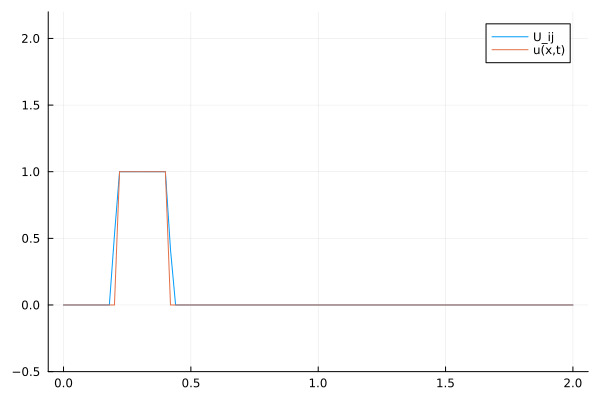
\includegraphics{Trabalho_final_AN_files/gifs/onda5-1}} &
%         \adjustbox{max width=\dimexpr\textwidth/3\relax, max height=\dimexpr\textheight/5\relax}{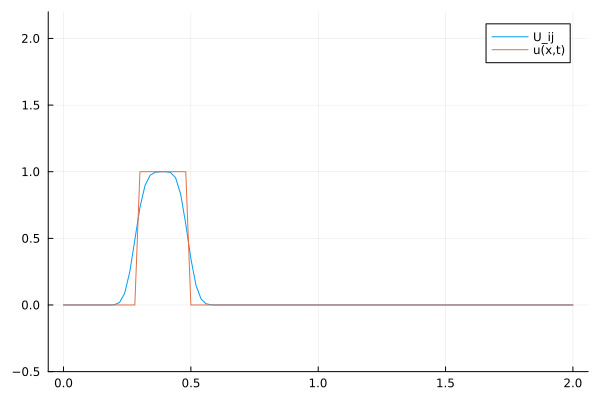
\includegraphics{Trabalho_final_AN_files/gifs/onda5-10}} &
%         \adjustbox{max width=\dimexpr\textwidth/3\relax, max height=\dimexpr\textheight/5\relax}{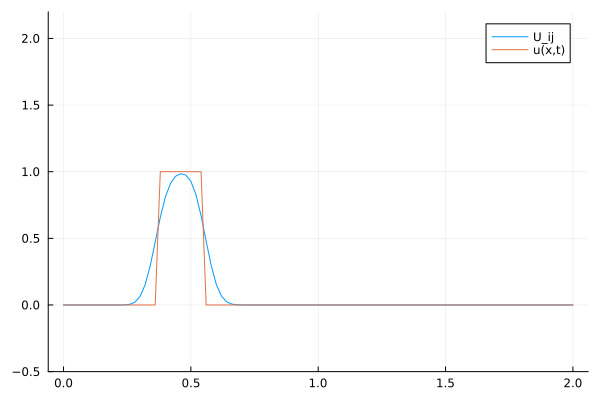
\includegraphics{Trabalho_final_AN_files/gifs/onda5-20}} \\

%         % --- Linha 2 ---
%         \adjustbox{max width=\dimexpr\textwidth/3\relax, max height=\dimexpr\textheight/5\relax}{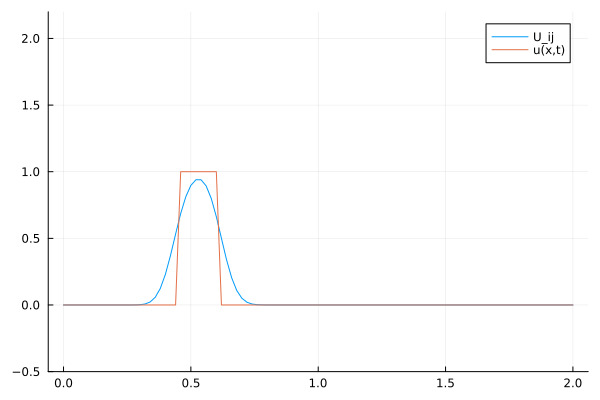
\includegraphics{Trabalho_final_AN_files/gifs/onda5-30}} &
%         \adjustbox{max width=\dimexpr\textwidth/3\relax, max height=\dimexpr\textheight/5\relax}{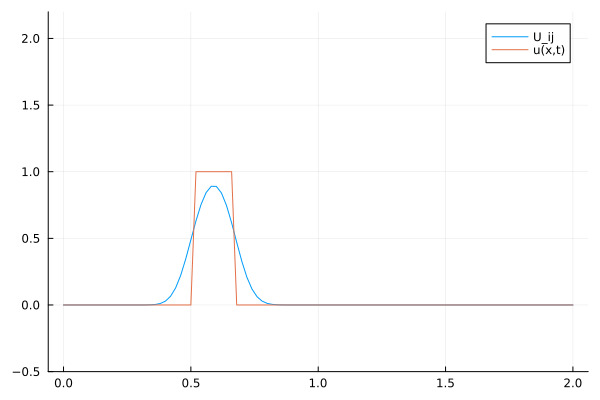
\includegraphics{Trabalho_final_AN_files/gifs/onda5-40}} &
%         \adjustbox{max width=\dimexpr\textwidth/3\relax, max height=\dimexpr\textheight/5\relax}{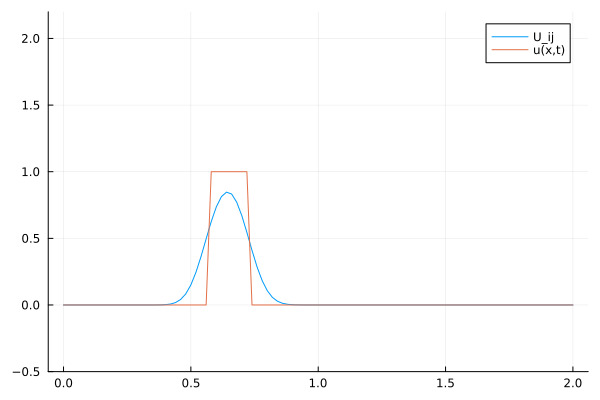
\includegraphics{Trabalho_final_AN_files/gifs/onda5-50}} \\

%         % --- Linha 3 ---
%         \adjustbox{max width=\dimexpr\textwidth/3\relax, max height=\dimexpr\textheight/5\relax}{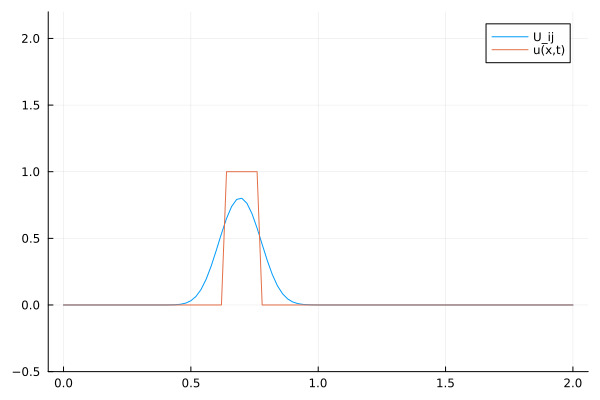
\includegraphics{Trabalho_final_AN_files/gifs/onda5-60}} &
%         \adjustbox{max width=\dimexpr\textwidth/3\relax, max height=\dimexpr\textheight/5\relax}{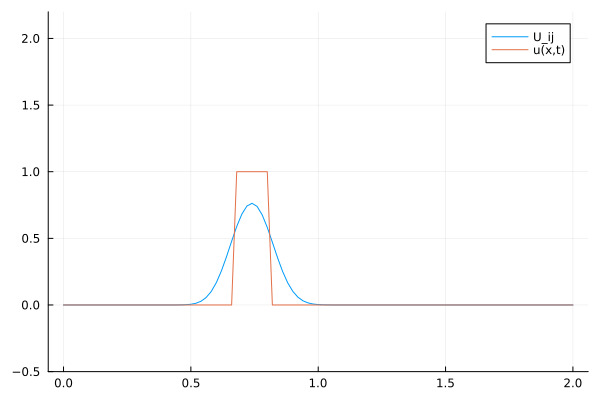
\includegraphics{Trabalho_final_AN_files/gifs/onda5-70}} &
%         \adjustbox{max width=\dimexpr\textwidth/3\relax, max height=\dimexpr\textheight/5\relax}{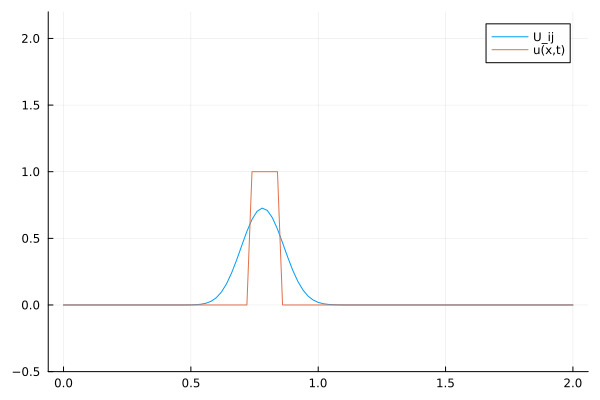
\includegraphics{Trabalho_final_AN_files/gifs/onda5-80}} \\
        
%         % --- Linha 4 --- 
        
%         % Se precisar de 15 imagens, você teria que usar 5 ondas (n=1 a 5) e os 15 frames
%         % Os frames seriam: 0, 15, 30, 45, 60, 75, 90, 105, 120, 135, 150, 165, 180, 195, 210, 225

%         % Para ter *exatamente* 15 imagens (5x3), precisamos de 15 frames.
%         % Os frames solicitados são 0, 15, ..., 225 (16 frames). 
%         % Adaptei para 15 frames: 0, 15, ..., 210, utilizando as primeiras 5 ondas. 
%         % Para incluir o frame 225, você precisaria de um grid 6x3 ou 5x4.
        
%         % Se quiser usar o frame 225, basta adicionar mais uma linha ao \begin{tabular}:
%         % --- Linha 6 (Opcional - se o grid fosse 6x3) ---
%         % \adjustbox{max width=\dimexpr\textwidth/3\relax, max height=\dimexpr\textheight/5\relax}{\includegraphics{Trabalho_final_AN_files/gifs/onda6-225}} & & \\
        
%     \end{tabular}
% \end{center}
        
  
        
    Novamente temos um efeito de suavização e dissipação.

    \hypertarget{b-condiuxe7uxe3o-inicial-suave}{%
\subsubsection{(b) Condição inicial
suave}}

    \begin{tcolorbox}[breakable, size=fbox, boxrule=1pt, pad at break*=1mm,colback=cellbackground, colframe=cellborder]
\prompt{In}{incolor}{ }{\boxspacing}
\begin{Verbatim}[commandchars=\\\{\}]
\PY{n}{u}\PY{p}{(}\PY{n}{x}\PY{p}{)}\PY{+w}{ }\PY{o}{=}\PY{+w}{ }\PY{n}{exp}\PY{p}{(}\PY{o}{\PYZhy{}}\PY{l+m+mi}{10}\PY{p}{(}\PY{l+m+mi}{4}\PY{n}{x}\PY{+w}{ }\PY{o}{\PYZhy{}}\PY{+w}{ }\PY{l+m+mi}{1}\PY{p}{)}\PY{o}{\PYZca{}}\PY{l+m+mi}{2}\PY{p}{)}
\end{Verbatim}
\end{tcolorbox}

            \begin{tcolorbox}[breakable, size=fbox, boxrule=.5pt, pad at break*=1mm, opacityfill=0]
\prompt{Out}{outcolor}{ }{\boxspacing}
\begin{Verbatim}[commandchars=\\\{\}]
u (generic function with 1 method)
\end{Verbatim}
\end{tcolorbox}
        
    \hypertarget{lax-wendroff}{%
\paragraph{Lax-Wendroff}}

    \begin{tcolorbox}[breakable, size=fbox, boxrule=1pt, pad at break*=1mm,colback=cellbackground, colframe=cellborder]
\prompt{In}{incolor}{ }{\boxspacing}
\begin{Verbatim}[commandchars=\\\{\}]
\PY{c}{\PYZsh{} Lax\PYZhy{}Wendroff}
\PY{n}{h}\PY{+w}{ }\PY{o}{=}\PY{+w}{ }\PY{l+m+mf}{0.02}
\PY{n}{k}\PY{+w}{ }\PY{o}{=}\PY{+w}{ }\PY{l+m+mf}{0.01}

\PY{n}{T}\PY{+w}{ }\PY{o}{=}\PY{+w}{ }\PY{l+m+mi}{100}

\PY{n}{domain}\PY{+w}{ }\PY{o}{=}\PY{+w}{ }\PY{l+m+mi}{0}\PY{o}{:}\PY{n}{h}\PY{o}{:}\PY{l+m+mi}{2}

\PY{n}{U0}\PY{+w}{ }\PY{o}{=}\PY{+w}{  }\PY{n}{u}\PY{o}{.}\PY{p}{(}\PY{n}{domain}\PY{p}{)}\PY{p}{;}

\PY{n}{ν}\PY{+w}{ }\PY{o}{=}\PY{+w}{ }\PY{n}{k}\PY{o}{/}\PY{n}{h}

\PY{n}{U}\PY{+w}{ }\PY{o}{=}\PY{+w}{ }\PY{p}{[}\PY{n}{U0}\PY{p}{]}


\PY{n}{M}\PY{+w}{ }\PY{o}{=}\PY{+w}{ }\PY{n}{length}\PY{p}{(}\PY{n}{U0}\PY{p}{)}

\PY{k}{for}\PY{+w}{ }\PY{n}{j}\PY{o}{=}\PY{l+m+mi}{1}\PY{o}{:}\PY{n}{T}
\PY{+w}{  }\PY{n}{Ujp1}\PY{+w}{ }\PY{o}{=}\PY{+w}{ }\PY{n}{zeros}\PY{p}{(}\PY{n}{M}\PY{p}{)}\PY{+w}{ }\PY{c}{\PYZsh{} Ut[0] = 0 por condição inicial}
\PY{+w}{  }\PY{n}{Uj}\PY{+w}{ }\PY{o}{=}\PY{+w}{ }\PY{n}{U}\PY{p}{[}\PY{n}{j}\PY{p}{]}
\PY{+w}{  }\PY{k}{for}\PY{+w}{ }\PY{n}{i}\PY{o}{=}\PY{l+m+mi}{2}\PY{o}{:}\PY{n}{M}\PY{o}{\PYZhy{}}\PY{l+m+mi}{1}\PY{+w}{  }\PY{c}{\PYZsh{} para os pontos jnterjores fazemos o esquema Lax\PYZhy{}Wendroff}
\PY{+w}{    }\PY{n}{xi}\PY{+w}{ }\PY{o}{=}\PY{+w}{ }\PY{n}{i}\PY{o}{*}\PY{n}{h}
\PY{+w}{    }\PY{n}{tj}\PY{+w}{ }\PY{o}{=}\PY{+w}{ }\PY{n}{j}\PY{o}{*}\PY{n}{k}
\PY{+w}{    }\PY{n}{va}\PY{+w}{ }\PY{o}{=}\PY{+w}{ }\PY{n}{ν}\PY{o}{*}\PY{n}{a}\PY{p}{(}\PY{n}{xi}\PY{p}{,}\PY{n}{tj}\PY{p}{)}
\PY{+w}{    }\PY{n}{Ujp1}\PY{p}{[}\PY{n}{i}\PY{p}{]}\PY{+w}{ }\PY{o}{=}\PY{+w}{ }\PY{n}{Uj}\PY{p}{[}\PY{n}{i}\PY{p}{]}\PY{+w}{ }\PY{o}{\PYZhy{}}\PY{+w}{ }\PY{n}{va}\PY{o}{/}\PY{l+m+mi}{2}\PY{o}{*}\PY{p}{(}\PY{n}{Uj}\PY{p}{[}\PY{n}{i}\PY{o}{+}\PY{l+m+mi}{1}\PY{p}{]}\PY{o}{\PYZhy{}}\PY{n}{Uj}\PY{p}{[}\PY{n}{i}\PY{o}{\PYZhy{}}\PY{l+m+mi}{1}\PY{p}{]}\PY{p}{)}\PY{+w}{ }\PY{o}{+}
\PY{+w}{                    }\PY{n}{va}\PY{o}{\PYZca{}}\PY{l+m+mi}{2}\PY{o}{/}\PY{l+m+mi}{2}\PY{o}{*}\PY{p}{(}\PY{n}{Uj}\PY{p}{[}\PY{n}{i}\PY{o}{+}\PY{l+m+mi}{1}\PY{p}{]}\PY{+w}{ }\PY{o}{\PYZhy{}}\PY{l+m+mi}{2}\PY{n}{Uj}\PY{p}{[}\PY{n}{i}\PY{p}{]}\PY{+w}{ }\PY{o}{+}\PY{+w}{ }\PY{n}{Uj}\PY{p}{[}\PY{n}{i}\PY{o}{\PYZhy{}}\PY{l+m+mi}{1}\PY{p}{]}\PY{p}{)}
\PY{+w}{  }\PY{k}{end}
\PY{+w}{  }\PY{n}{push!}\PY{p}{(}\PY{n}{U}\PY{p}{,}\PY{+w}{ }\PY{n}{Ujp1}\PY{p}{)}
\PY{k}{end}
\end{Verbatim}
\end{tcolorbox}

    \begin{tcolorbox}[breakable, size=fbox, boxrule=1pt, pad at break*=1mm,colback=cellbackground, colframe=cellborder]
\prompt{In}{incolor}{ }{\boxspacing}
\begin{Verbatim}[commandchars=\\\{\}]
\PY{n}{graficos}\PY{+w}{ }\PY{o}{=}\PY{+w}{ }\PY{p}{[}\PY{p}{]}
\PY{k}{for}\PY{+w}{ }\PY{n}{t}\PY{o}{=}\PY{p}{[}\PY{l+m+mi}{1}\PY{p}{,}\PY{l+m+mi}{11}\PY{p}{,}\PY{l+m+mi}{51}\PY{p}{,}\PY{l+m+mi}{101}\PY{+w}{ }\PY{p}{]}
\PY{+w}{  }\PY{n}{tt}\PY{+w}{ }\PY{o}{=}\PY{+w}{ }\PY{p}{(}\PY{n}{t}\PY{o}{\PYZhy{}}\PY{l+m+mi}{1}\PY{p}{)}\PY{o}{*}\PY{n}{k}
\PY{+w}{  }\PY{n}{p}\PY{+w}{ }\PY{o}{=}\PY{+w}{ }\PY{n}{plot}\PY{p}{(}\PY{n}{domain}\PY{p}{,}\PY{+w}{ }\PY{n}{U}\PY{p}{[}\PY{n}{t}\PY{p}{]}\PY{p}{,}\PY{+w}{ }\PY{n}{ylim}\PY{o}{=}\PY{p}{(}\PY{o}{\PYZhy{}}\PY{l+m+mf}{0.5}\PY{p}{,}\PY{l+m+mf}{1.2}\PY{p}{)}\PY{p}{,}\PY{+w}{ }\PY{n}{label}\PY{o}{=}\PY{l+s}{\PYZdq{}}\PY{l+s}{U\PYZus{}ij}\PY{l+s}{\PYZdq{}}\PY{p}{,}\PY{+w}{ }\PY{n}{title}\PY{o}{=}\PY{l+s}{\PYZdq{}}\PY{l+s}{t=}\PY{l+s+si}{\PYZdl{}tt}\PY{l+s}{\PYZdq{}}\PY{p}{)}
\PY{+w}{  }\PY{n}{solu}\PY{p}{(}\PY{n}{z}\PY{p}{)}\PY{+w}{ }\PY{o}{=}\PY{+w}{ }\PY{n}{z}\PY{o}{\PYZhy{}}\PY{+w}{ }\PY{n}{tt}\PY{o}{/}\PY{p}{(}\PY{l+m+mi}{1}\PY{o}{+}\PY{n}{z}\PY{o}{\PYZca{}}\PY{l+m+mi}{2}\PY{p}{)}
\PY{+w}{  }\PY{n}{plot!}\PY{p}{(}\PY{n}{p}\PY{p}{,}\PY{+w}{ }\PY{n}{domain}\PY{p}{,}\PY{+w}{ }\PY{n}{u}\PY{o}{.}\PY{p}{(}\PY{n}{solu}\PY{o}{.}\PY{p}{(}\PY{n}{domain}\PY{p}{)}\PY{p}{)}\PY{p}{,}\PY{+w}{ }\PY{n}{label}\PY{o}{=}\PY{l+s}{\PYZdq{}}\PY{l+s}{u(x,t)}\PY{l+s}{\PYZdq{}}\PY{p}{)}
\PY{+w}{  }\PY{n}{push!}\PY{p}{(}\PY{n}{graficos}\PY{p}{,}\PY{+w}{ }\PY{n}{p}\PY{p}{)}
\PY{k}{end}
\PY{n}{plot}\PY{p}{(}\PY{n}{graficos}\PY{o}{...}\PY{p}{;}\PY{+w}{ }\PY{n}{layout}\PY{o}{=}\PY{n+nd}{@layout}\PY{p}{(}\PY{p}{[}\PY{n}{°}\PY{+w}{ }\PY{n}{°}\PY{p}{;}\PY{+w}{ }\PY{n}{°}\PY{+w}{ }\PY{n}{°}\PY{p}{]}\PY{p}{)}\PY{p}{,}\PY{+w}{ }\PY{n}{size}\PY{o}{=}\PY{p}{(}\PY{l+m+mi}{1200}\PY{p}{,}\PY{l+m+mi}{600}\PY{p}{)}\PY{p}{)}
\end{Verbatim}
\end{tcolorbox}
 
            
\prompt{Out}{outcolor}{ }{}
    
    \begin{center}
    \adjustimage{max size={0.9\linewidth}{0.9\paperheight}}{Trabalho_final_AN_files/Trabalho_final_AN_59_0.pdf}
    \end{center}
    { \hspace*{\fill} \\}
    
 

% Para centralizar a tabela na página
% \begin{center}
%     % Definimos um array de 3 colunas, todas centralizadas (c)
%     % A largura da coluna será automaticamente calculada.
%     % A largura total da tabela é ajustada para \textwidth (largura do texto)
%     % Ajustamos o espaçamento entre as colunas (colsep) e linhas (rowsep) para ficar mais apertado, se necessário.
%     \setlength{\tabcolsep}{1pt} % Espaçamento horizontal entre colunas
%     \renewcommand{\arraystretch}{0.5} % Espaçamento vertical entre linhas
    
%     \begin{tabular}{ccc} % 3 colunas

%         % --- Linha 1 ---
%         % As imagens são ajustadas para ter 1/3 da largura do texto menos o espaçamento6
%         % Você pode ajustar a escala (\scalebox) se for mais conveniente6
%         \adjustbox{max width=\dimexpr\textwidth/3\relax, max height=\dimexpr\textheight/5\relax}{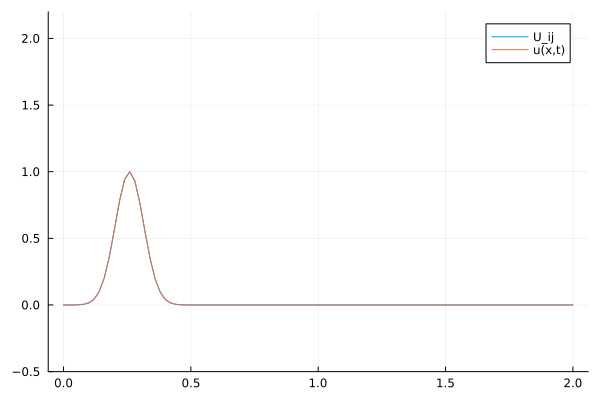
\includegraphics{Trabalho_final_AN_files/gifs/onda6-1}} &
%         \adjustbox{max width=\dimexpr\textwidth/3\relax, max height=\dimexpr\textheight/5\relax}{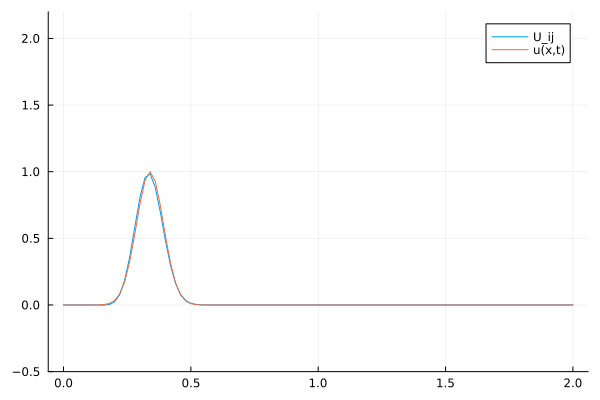
\includegraphics{Trabalho_final_AN_files/gifs/onda6-10}} &
%         \adjustbox{max width=\dimexpr\textwidth/3\relax, max height=\dimexpr\textheight/5\relax}{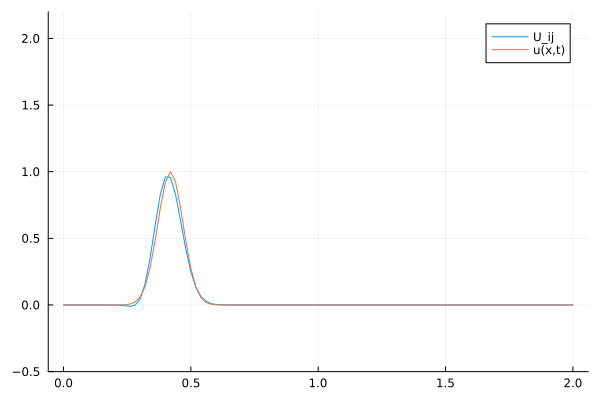
\includegraphics{Trabalho_final_AN_files/gifs/onda6-20}} \\
%         % --- Linha 2 --6
%         \adjustbox{max width=\dimexpr\textwidth/3\relax, max height=\dimexpr\textheight/5\relax}{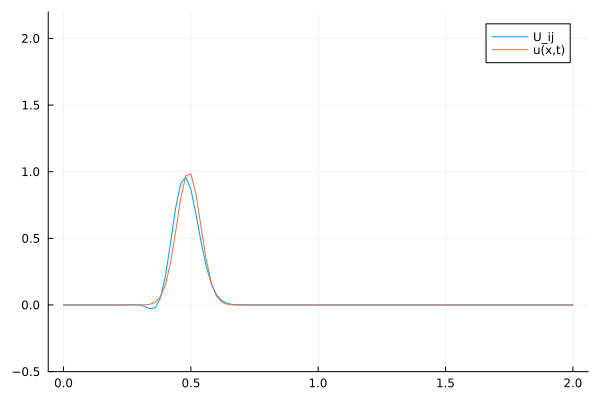
\includegraphics{Trabalho_final_AN_files/gifs/onda6-30}} &
%         \adjustbox{max width=\dimexpr\textwidth/3\relax, max height=\dimexpr\textheight/5\relax}{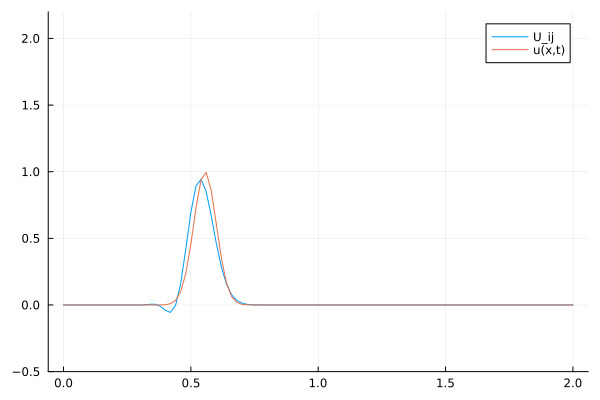
\includegraphics{Trabalho_final_AN_files/gifs/onda6-40}} &
%         \adjustbox{max width=\dimexpr\textwidth/3\relax, max height=\dimexpr\textheight/5\relax}{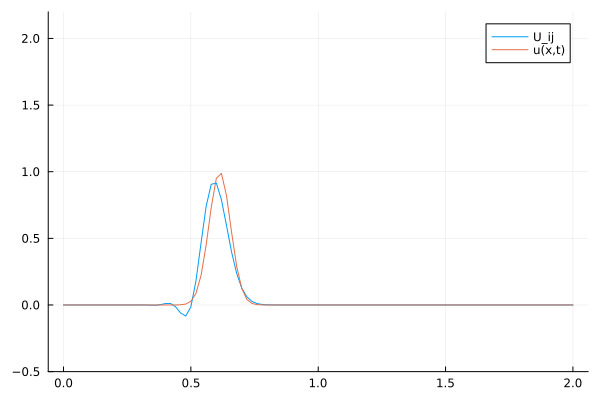
\includegraphics{Trabalho_final_AN_files/gifs/onda6-50}} \\

%         % --- Linha 3 ---
%         \adjustbox{max width=\dimexpr\textwidth/3\relax, max height=\dimexpr\textheight/5\relax}{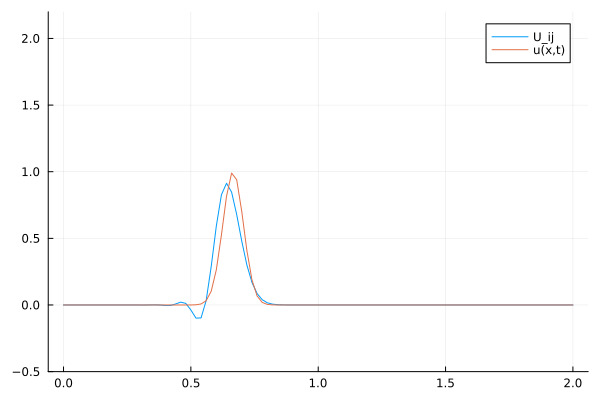
\includegraphics{Trabalho_final_AN_files/gifs/onda6-60}} &
%         \adjustbox{max width=\dimexpr\textwidth/3\relax, max height=\dimexpr\textheight/5\relax}{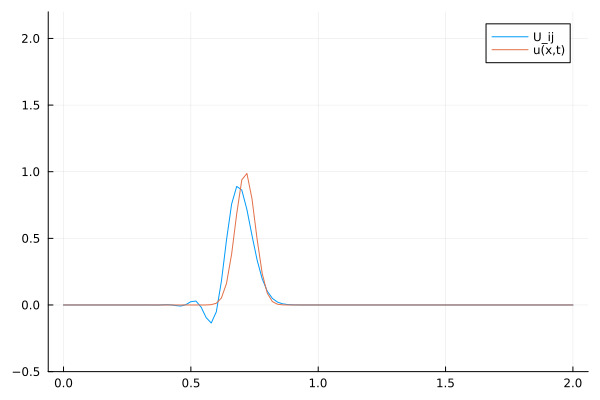
\includegraphics{Trabalho_final_AN_files/gifs/onda6-70}} &
%         \adjustbox{max width=\dimexpr\textwidth/3\relax, max height=\dimexpr\textheight/5\relax}{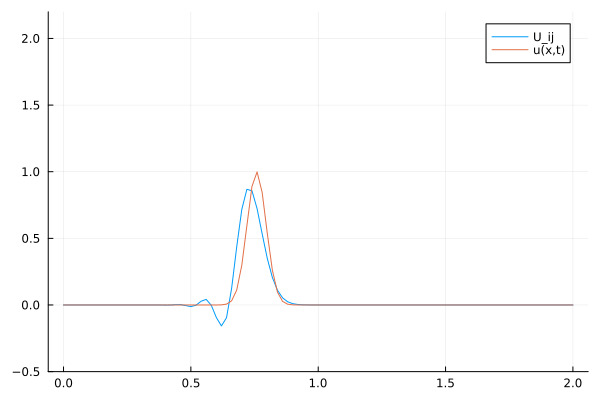
\includegraphics{Trabalho_final_AN_files/gifs/onda6-80}} \\
        
%         % --- Linha 4 --- 
        
%         % Se precisar de 15 imagens, você teria que usar 5 ondas (n=1 a 5) e os 15 frames
%         % Os frames seriam: 0, 15, 30, 45, 60, 75, 90, 105, 120, 135, 150, 165, 180, 195, 210, 225

%         % Para ter *exatamente* 15 imagens (5x3), precisamos de 15 frames.
%         % Os frames solicitados são 0, 15, ..., 225 (16 frames). 
%         % Adaptei para 15 frames: 0, 15, ..., 210, utilizando as primeiras 5 ondas. 
%         % Para incluir o frame 225, você precisaria de um grid 6x3 ou 5x4.
        
%         % Se quiser usar o frame 225, basta adicionar mais uma linha ao \begin{tabular}:
%         % --- Linha 6 (Opcional - se o grid fosse 6x3) ---
%         % \adjustbox{max width=\dimexpr\textwidth/3\relax, max height=\dimexpr\textheight/5\relax}{\includegraphics{Trabalho_final_AN_files/gifs/onda6-225}} & & \\
        
%     \end{tabular}
% \end{center}
        

        
    \hypertarget{esquema-impluxedcito-de-primeira-ordem}{%
\paragraph{Esquema implícito de primeira
ordem}}

    \begin{figure}
\centering
\caption{image.png}
\end{figure}

    \[U_{i,j} = (1+\nu a)U_{i,j+1} - \nu aU_{i-1,j+1}\]

    \begin{tcolorbox}[breakable, size=fbox, boxrule=1pt, pad at break*=1mm,colback=cellbackground, colframe=cellborder]
\prompt{In}{incolor}{ }{\boxspacing}
\begin{Verbatim}[commandchars=\\\{\}]
\PY{c}{\PYZsh{} Implicito Primeira Ordem}
\PY{n}{h}\PY{+w}{ }\PY{o}{=}\PY{+w}{ }\PY{l+m+mf}{0.02}
\PY{n}{k}\PY{+w}{ }\PY{o}{=}\PY{+w}{ }\PY{l+m+mf}{0.01}

\PY{n}{T}\PY{+w}{ }\PY{o}{=}\PY{+w}{ }\PY{l+m+mi}{100}

\PY{n}{domain}\PY{+w}{ }\PY{o}{=}\PY{+w}{ }\PY{l+m+mi}{0}\PY{o}{:}\PY{n}{h}\PY{o}{:}\PY{l+m+mi}{2}

\PY{n}{U0}\PY{+w}{ }\PY{o}{=}\PY{+w}{  }\PY{n}{u}\PY{o}{.}\PY{p}{(}\PY{n}{domain}\PY{p}{)}\PY{p}{;}


\PY{n}{U}\PY{+w}{ }\PY{o}{=}\PY{+w}{ }\PY{p}{[}\PY{n}{U0}\PY{p}{]}
\PY{n}{ν}\PY{+w}{ }\PY{o}{=}\PY{+w}{ }\PY{n}{k}\PY{o}{/}\PY{n}{h}

\PY{n}{M}\PY{+w}{ }\PY{o}{=}\PY{+w}{ }\PY{n}{length}\PY{p}{(}\PY{n}{U0}\PY{p}{)}

\PY{k}{for}\PY{+w}{ }\PY{n}{j}\PY{o}{=}\PY{l+m+mi}{1}\PY{o}{:}\PY{n}{T}
\PY{+w}{  }\PY{n}{Uj}\PY{+w}{ }\PY{o}{=}\PY{+w}{ }\PY{n}{U}\PY{p}{[}\PY{n}{j}\PY{p}{]}
\PY{+w}{  }\PY{n}{diag}\PY{+w}{ }\PY{o}{=}\PY{+w}{ }\PY{n}{ones}\PY{p}{(}\PY{n}{M}\PY{p}{)}
\PY{+w}{  }\PY{n}{subdiag}\PY{+w}{ }\PY{o}{=}\PY{+w}{ }\PY{n}{zeros}\PY{p}{(}\PY{n}{M}\PY{o}{\PYZhy{}}\PY{l+m+mi}{1}\PY{p}{)}
\PY{+w}{  }\PY{k}{for}\PY{+w}{ }\PY{n}{i}\PY{o}{=}\PY{l+m+mi}{1}\PY{o}{:}\PY{n}{M}\PY{o}{\PYZhy{}}\PY{l+m+mi}{1}
\PY{+w}{    }\PY{n}{xi}\PY{+w}{ }\PY{o}{=}\PY{+w}{ }\PY{p}{(}\PY{n}{i}\PY{o}{+}\PY{l+m+mi}{1}\PY{p}{)}\PY{o}{*}\PY{n}{h}
\PY{+w}{    }\PY{n}{tj}\PY{+w}{ }\PY{o}{=}\PY{+w}{ }\PY{n}{j}\PY{o}{*}\PY{n}{k}
\PY{+w}{    }\PY{n}{va}\PY{+w}{ }\PY{o}{=}\PY{+w}{ }\PY{n}{ν}\PY{o}{*}\PY{n}{a}\PY{p}{(}\PY{n}{xi}\PY{p}{,}\PY{n}{tj}\PY{p}{)}
\PY{+w}{    }\PY{n}{diag}\PY{p}{[}\PY{n}{i}\PY{o}{+}\PY{l+m+mi}{1}\PY{p}{]}\PY{+w}{ }\PY{o}{=}\PY{+w}{ }\PY{l+m+mi}{1}\PY{+w}{ }\PY{o}{+}\PY{+w}{ }\PY{n}{va}
\PY{+w}{    }\PY{n}{subdiag}\PY{p}{[}\PY{n}{i}\PY{p}{]}\PY{+w}{ }\PY{o}{=}\PY{+w}{ }\PY{o}{\PYZhy{}}\PY{n}{va}
\PY{+w}{  }\PY{k}{end}
\PY{+w}{  }\PY{n}{A}\PY{+w}{ }\PY{o}{=}\PY{+w}{ }\PY{n}{Tridiagonal}\PY{p}{(}\PY{n}{subdiag}\PY{p}{,}\PY{+w}{ }\PY{n}{diag}\PY{p}{,}\PY{+w}{ }\PY{n}{zeros}\PY{p}{(}\PY{n}{M}\PY{o}{\PYZhy{}}\PY{l+m+mi}{1}\PY{p}{)}\PY{p}{)}
\PY{+w}{  }\PY{n}{Ujp1}\PY{+w}{ }\PY{o}{=}\PY{+w}{ }\PY{n}{A}\PY{o}{\PYZbs{}}\PY{n}{Uj}
\PY{+w}{  }\PY{n}{push!}\PY{p}{(}\PY{n}{U}\PY{p}{,}\PY{+w}{ }\PY{n}{Ujp1}\PY{p}{)}
\PY{k}{end}
\end{Verbatim}
\end{tcolorbox}

    \begin{tcolorbox}[breakable, size=fbox, boxrule=1pt, pad at break*=1mm,colback=cellbackground, colframe=cellborder]
\prompt{In}{incolor}{ }{\boxspacing}
\begin{Verbatim}[commandchars=\\\{\}]
\PY{n}{graficos}\PY{+w}{ }\PY{o}{=}\PY{+w}{ }\PY{p}{[}\PY{p}{]}
\PY{k}{for}\PY{+w}{ }\PY{n}{t}\PY{o}{=}\PY{p}{[}\PY{l+m+mi}{1}\PY{p}{,}\PY{l+m+mi}{11}\PY{p}{,}\PY{l+m+mi}{51}\PY{p}{,}\PY{l+m+mi}{101}\PY{+w}{ }\PY{p}{]}
\PY{+w}{  }\PY{n}{tt}\PY{+w}{ }\PY{o}{=}\PY{+w}{ }\PY{p}{(}\PY{n}{t}\PY{o}{\PYZhy{}}\PY{l+m+mi}{1}\PY{p}{)}\PY{o}{*}\PY{n}{k}
\PY{+w}{  }\PY{n}{p}\PY{+w}{ }\PY{o}{=}\PY{+w}{ }\PY{n}{plot}\PY{p}{(}\PY{n}{domain}\PY{p}{,}\PY{+w}{ }\PY{n}{U}\PY{p}{[}\PY{n}{t}\PY{p}{]}\PY{p}{,}\PY{+w}{ }\PY{n}{ylim}\PY{o}{=}\PY{p}{(}\PY{o}{\PYZhy{}}\PY{l+m+mf}{0.5}\PY{p}{,}\PY{l+m+mf}{1.2}\PY{p}{)}\PY{p}{,}\PY{+w}{ }\PY{n}{label}\PY{o}{=}\PY{l+s}{\PYZdq{}}\PY{l+s}{U\PYZus{}ij}\PY{l+s}{\PYZdq{}}\PY{p}{,}\PY{+w}{ }\PY{n}{title}\PY{o}{=}\PY{l+s}{\PYZdq{}}\PY{l+s}{t=}\PY{l+s+si}{\PYZdl{}tt}\PY{l+s}{\PYZdq{}}\PY{p}{)}
\PY{+w}{  }\PY{n}{solu}\PY{p}{(}\PY{n}{z}\PY{p}{)}\PY{+w}{ }\PY{o}{=}\PY{+w}{ }\PY{n}{z}\PY{o}{\PYZhy{}}\PY{+w}{ }\PY{n}{tt}\PY{o}{/}\PY{p}{(}\PY{l+m+mi}{1}\PY{o}{+}\PY{n}{z}\PY{o}{\PYZca{}}\PY{l+m+mi}{2}\PY{p}{)}
\PY{+w}{  }\PY{n}{plot!}\PY{p}{(}\PY{n}{p}\PY{p}{,}\PY{+w}{ }\PY{n}{domain}\PY{p}{,}\PY{+w}{ }\PY{n}{u}\PY{o}{.}\PY{p}{(}\PY{n}{solu}\PY{o}{.}\PY{p}{(}\PY{n}{domain}\PY{p}{)}\PY{p}{)}\PY{p}{,}\PY{+w}{ }\PY{n}{label}\PY{o}{=}\PY{l+s}{\PYZdq{}}\PY{l+s}{u(x,t)}\PY{l+s}{\PYZdq{}}\PY{p}{)}
\PY{+w}{  }\PY{n}{push!}\PY{p}{(}\PY{n}{graficos}\PY{p}{,}\PY{+w}{ }\PY{n}{p}\PY{p}{)}
\PY{k}{end}
\PY{n}{plot}\PY{p}{(}\PY{n}{graficos}\PY{o}{...}\PY{p}{;}\PY{+w}{ }\PY{n}{layout}\PY{o}{=}\PY{n+nd}{@layout}\PY{p}{(}\PY{p}{[}\PY{n}{°}\PY{+w}{ }\PY{n}{°}\PY{p}{;}\PY{+w}{ }\PY{n}{°}\PY{+w}{ }\PY{n}{°}\PY{p}{]}\PY{p}{)}\PY{p}{,}\PY{+w}{ }\PY{n}{size}\PY{o}{=}\PY{p}{(}\PY{l+m+mi}{1200}\PY{p}{,}\PY{l+m+mi}{600}\PY{p}{)}\PY{p}{)}
\end{Verbatim}
\end{tcolorbox}
 
            
\prompt{Out}{outcolor}{ }{}
    
    \begin{center}
    \adjustimage{max size={0.9\linewidth}{0.9\paperheight}}{Trabalho_final_AN_files/Trabalho_final_AN_65_0.pdf}
    \end{center}
    { \hspace*{\fill} \\}



% Para centralizar a tabela na página
% \begin{center}
%     % Definimos um array de 3 colunas, todas centralizadas (c)
%     % A largura da coluna será automaticamente calculada.
%     % A largura total da tabela é ajustada para \textwidth (largura do texto)
%     % Ajustamos o espaçamento entre as colunas (colsep) e linhas (rowsep) para ficar mais apertado, se necessário.
%     \setlength{\tabcolsep}{1pt} % Espaçamento horizontal entre colunas
%     \renewcommand{\arraystretch}{0.5} % Espaçamento vertical entre linhas
    
%     \begin{tabular}{ccc} % 3 colunas

%         % --- Linha 1 ---
%         % As imagens são ajustadas para ter 1/3 da largura do texto menos o espaçamento6
%         % Você pode ajustar a escala (\scalebox) se for mais conveniente6
%         \adjustbox{max width=\dimexpr\textwidth/3\relax, max height=\dimexpr\textheight/5\relax}{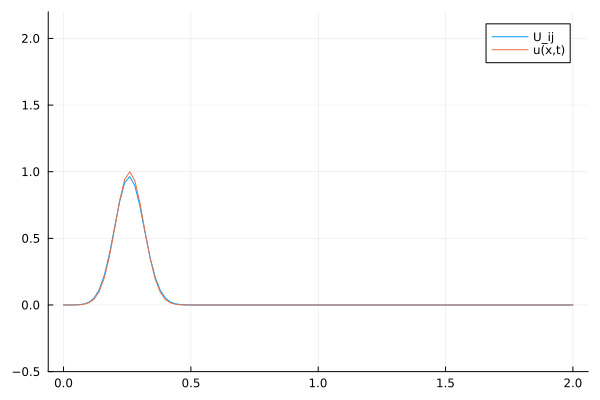
\includegraphics{Trabalho_final_AN_files/gifs/onda7-1}} &
%         \adjustbox{max width=\dimexpr\textwidth/3\relax, max height=\dimexpr\textheight/5\relax}{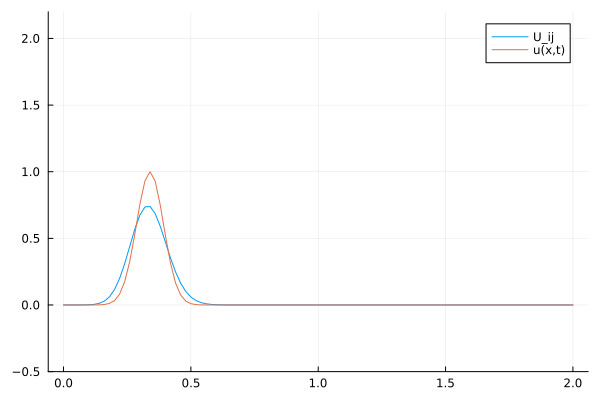
\includegraphics{Trabalho_final_AN_files/gifs/onda7-10}} &
%         \adjustbox{max width=\dimexpr\textwidth/3\relax, max height=\dimexpr\textheight/5\relax}{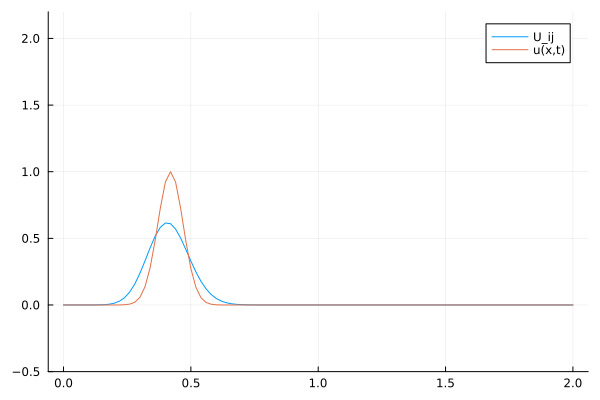
\includegraphics{Trabalho_final_AN_files/gifs/onda7-20}} \\
%         % --- Linha 2 --6
%         \adjustbox{max width=\dimexpr\textwidth/3\relax, max height=\dimexpr\textheight/5\relax}{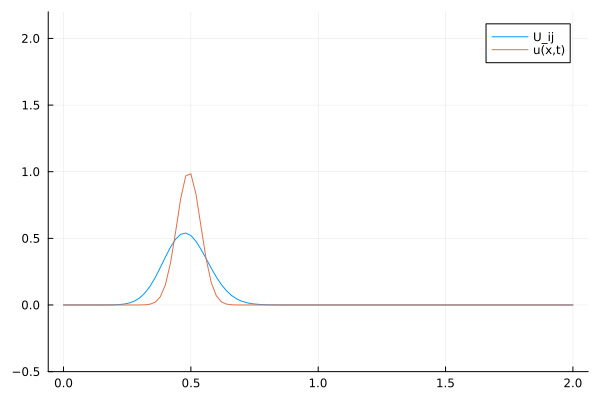
\includegraphics{Trabalho_final_AN_files/gifs/onda7-30}} &
%         \adjustbox{max width=\dimexpr\textwidth/3\relax, max height=\dimexpr\textheight/5\relax}{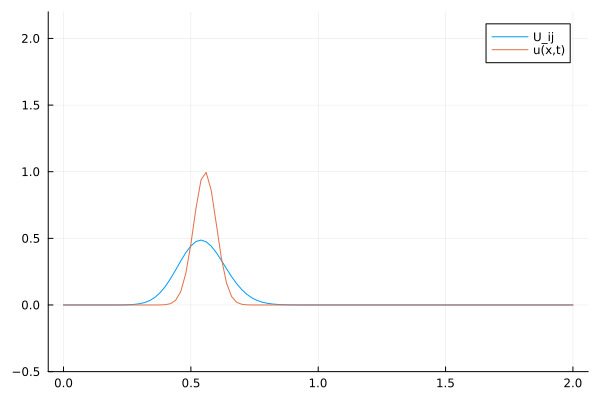
\includegraphics{Trabalho_final_AN_files/gifs/onda7-40}} &
%         \adjustbox{max width=\dimexpr\textwidth/3\relax, max height=\dimexpr\textheight/5\relax}{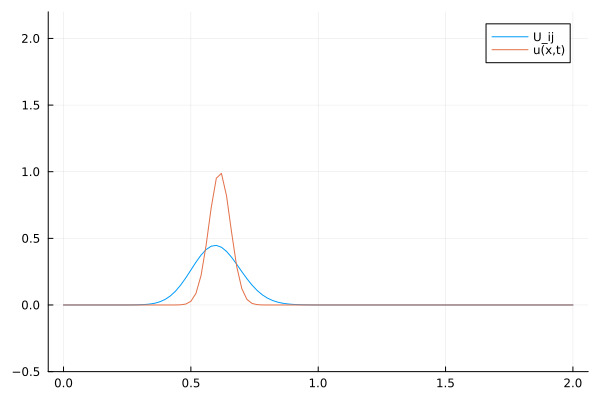
\includegraphics{Trabalho_final_AN_files/gifs/onda7-50}} \\

%         % --- Linha 3 ---
%         \adjustbox{max width=\dimexpr\textwidth/3\relax, max height=\dimexpr\textheight/5\relax}{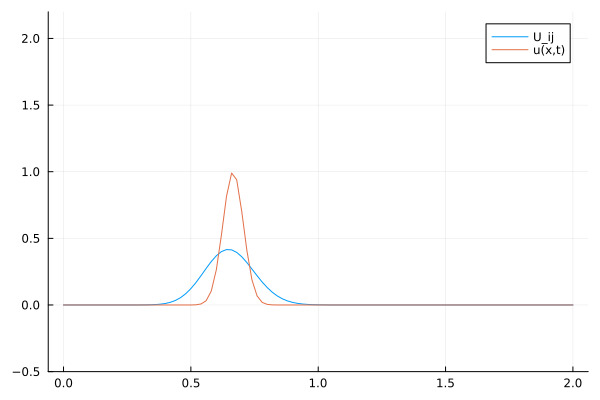
\includegraphics{Trabalho_final_AN_files/gifs/onda7-60}} &
%         \adjustbox{max width=\dimexpr\textwidth/3\relax, max height=\dimexpr\textheight/5\relax}{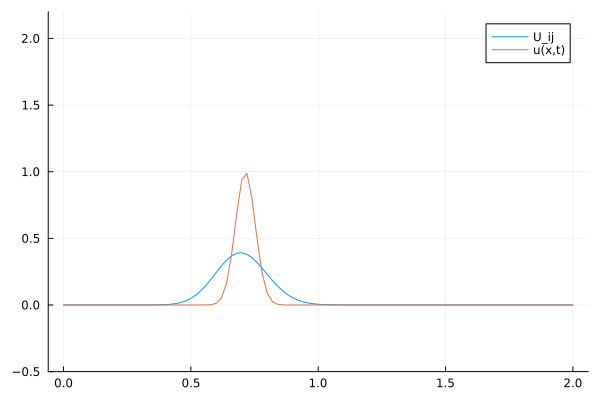
\includegraphics{Trabalho_final_AN_files/gifs/onda7-70}} &
%         \adjustbox{max width=\dimexpr\textwidth/3\relax, max height=\dimexpr\textheight/5\relax}{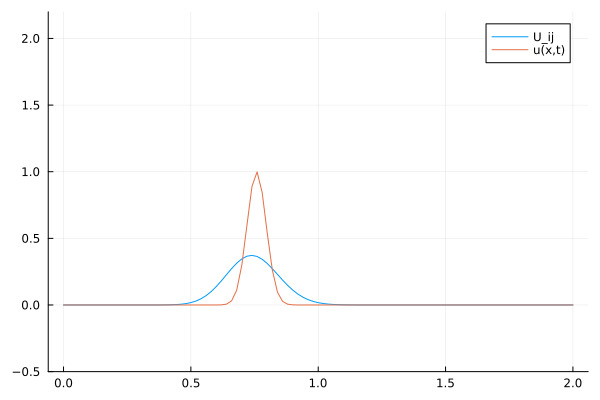
\includegraphics{Trabalho_final_AN_files/gifs/onda7-80}} \\
        
%         % --- Linha 4 --- 
        
%         % Se precisar de 15 imagens, você teria que usar 5 ondas (n=1 a 5) e os 15 frames
%         % Os frames seriam: 0, 15, 30, 45, 60, 75, 90, 105, 120, 135, 150, 165, 180, 195, 210, 225

%         % Para ter *exatamente* 15 imagens (5x3), precisamos de 15 frames.
%         % Os frames solicitados são 0, 15, ..., 225 (16 frames). 
%         % Adaptei para 15 frames: 0, 15, ..., 210, utilizando as primeiras 5 ondas. 
%         % Para incluir o frame 225, você precisaria de um grid 6x3 ou 5x4.
        
%         % Se quiser usar o frame 225, basta adicionar mais uma linha ao \begin{tabular}:
%         % --- Linha 6 (Opcional - se o grid fosse 6x3) ---
%         % \adjustbox{max width=\dimexpr\textwidth/3\relax, max height=\dimexpr\textheight/5\relax}{\includegraphics{Trabalho_final_AN_files/gifs/onda6-225}} & & \\
        
%     \end{tabular}
% \end{center}
        
    \hypertarget{muxe9todo-box}{%
\paragraph{Método Box}}

    \begin{figure}
\centering
\caption{image.png}
\end{figure}

    \[U_{i+1,j+1} + \frac{1-\nu a}{1+\nu a}U_{i,j+1} = U_{i,j} + \frac{1-\nu a}{1+\nu a}U_{i+1,j}\]

    \begin{tcolorbox}[breakable, size=fbox, boxrule=1pt, pad at break*=1mm,colback=cellbackground, colframe=cellborder]
\prompt{In}{incolor}{ }{\boxspacing}
\begin{Verbatim}[commandchars=\\\{\}]
\PY{c}{\PYZsh{} Método Box}
\PY{n}{h}\PY{+w}{ }\PY{o}{=}\PY{+w}{ }\PY{l+m+mf}{0.02}
\PY{n}{k}\PY{+w}{ }\PY{o}{=}\PY{+w}{ }\PY{l+m+mf}{0.01}
\PY{n}{T}\PY{+w}{ }\PY{o}{=}\PY{+w}{ }\PY{l+m+mi}{100}
\PY{n}{domain}\PY{+w}{ }\PY{o}{=}\PY{+w}{ }\PY{l+m+mi}{0}\PY{o}{:}\PY{n}{h}\PY{o}{:}\PY{l+m+mi}{2}

\PY{n}{U0}\PY{+w}{ }\PY{o}{=}\PY{+w}{  }\PY{n}{u}\PY{o}{.}\PY{p}{(}\PY{n}{domain}\PY{p}{)}\PY{p}{;}
\PY{n}{U}\PY{+w}{ }\PY{o}{=}\PY{+w}{ }\PY{p}{[}\PY{n}{U0}\PY{p}{]}
\PY{n}{ν}\PY{+w}{ }\PY{o}{=}\PY{+w}{ }\PY{n}{k}\PY{o}{/}\PY{n}{h}

\PY{n}{M}\PY{+w}{ }\PY{o}{=}\PY{+w}{ }\PY{n}{length}\PY{p}{(}\PY{n}{U0}\PY{p}{)}
\PY{k}{for}\PY{+w}{ }\PY{n}{j}\PY{o}{=}\PY{l+m+mi}{1}\PY{o}{:}\PY{n}{T}
\PY{+w}{  }\PY{n}{Uj}\PY{+w}{ }\PY{o}{=}\PY{+w}{ }\PY{n}{U}\PY{p}{[}\PY{n}{j}\PY{p}{]}

\PY{+w}{  }\PY{n}{Ujp1}\PY{+w}{ }\PY{o}{=}\PY{+w}{ }\PY{n}{zeros}\PY{p}{(}\PY{n}{M}\PY{p}{)}
\PY{+w}{  }\PY{n}{diagA}\PY{+w}{ }\PY{o}{=}\PY{+w}{ }\PY{n}{ones}\PY{p}{(}\PY{n}{M}\PY{p}{)}
\PY{+w}{  }\PY{n}{subdiagB}\PY{+w}{ }\PY{o}{=}\PY{+w}{ }\PY{n}{zeros}\PY{p}{(}\PY{n}{M}\PY{p}{)}
\PY{+w}{  }\PY{k}{for}\PY{+w}{ }\PY{n}{i}\PY{o}{=}\PY{l+m+mi}{1}\PY{o}{:}\PY{n}{M}\PY{o}{\PYZhy{}}\PY{l+m+mi}{1}
\PY{+w}{    }\PY{n}{xi}\PY{+w}{ }\PY{o}{=}\PY{+w}{ }\PY{p}{(}\PY{n}{i}\PY{o}{\PYZhy{}}\PY{l+m+mi}{1}\PY{p}{)}\PY{o}{*}\PY{n}{h}\PY{+w}{  }\PY{c}{\PYZsh{} Correção: índice começa em 0}
\PY{+w}{    }\PY{n}{tj}\PY{+w}{ }\PY{o}{=}\PY{+w}{ }\PY{p}{(}\PY{n}{j}\PY{o}{\PYZhy{}}\PY{l+m+mi}{1}\PY{p}{)}\PY{o}{*}\PY{n}{k}
\PY{+w}{    }\PY{n}{va}\PY{+w}{ }\PY{o}{=}\PY{+w}{ }\PY{n}{ν}\PY{o}{*}\PY{n}{a}\PY{p}{(}\PY{n}{xi}\PY{p}{,}\PY{n}{tj}\PY{p}{)}
\PY{+w}{    }\PY{n}{λ}\PY{+w}{ }\PY{o}{=}\PY{+w}{ }\PY{p}{(}\PY{l+m+mi}{1}\PY{+w}{ }\PY{o}{\PYZhy{}}\PY{+w}{ }\PY{n}{va}\PY{p}{)}\PY{o}{/}\PY{p}{(}\PY{l+m+mi}{1}\PY{+w}{ }\PY{o}{+}\PY{+w}{ }\PY{n}{va}\PY{p}{)}
\PY{+w}{    }\PY{k}{if}\PY{+w}{ }\PY{n}{i}\PY{+w}{ }\PY{o}{==}\PY{+w}{ }\PY{l+m+mi}{1}
\PY{+w}{    }\PY{c}{\PYZsh{} Para i=1: U\PYZus{}\PYZob{}1,j+1\PYZcb{} = 0 (condição de contorno)}
\PY{+w}{    }\PY{c}{\PYZsh{} Equação: U\PYZus{}\PYZob{}2,j+1\PYZcb{} + λ * 0 = U\PYZus{}\PYZob{}1,j\PYZcb{} + λ * U\PYZus{}\PYZob{}2,j\PYZcb{}}
\PY{+w}{        }\PY{n}{Ujp1}\PY{p}{[}\PY{l+m+mi}{2}\PY{p}{]}\PY{+w}{ }\PY{o}{=}\PY{+w}{ }\PY{n}{Uj}\PY{p}{[}\PY{l+m+mi}{1}\PY{p}{]}\PY{+w}{ }\PY{o}{+}\PY{+w}{ }\PY{n}{λ}\PY{+w}{ }\PY{o}{*}\PY{+w}{ }\PY{n}{Uj}\PY{p}{[}\PY{l+m+mi}{2}\PY{p}{]}
\PY{+w}{    }\PY{k}{else}
\PY{+w}{        }\PY{c}{\PYZsh{} Para i\PYZgt{}1: U\PYZus{}\PYZob{}i+1,j+1\PYZcb{} + λ * U\PYZus{}\PYZob{}i,j+1\PYZcb{} = U\PYZus{}\PYZob{}i,j\PYZcb{} + λ * U\PYZus{}\PYZob{}i+1,j\PYZcb{}}
\PY{+w}{        }\PY{c}{\PYZsh{} Isolando U\PYZus{}\PYZob{}i+1,j+1\PYZcb{}:}
\PY{+w}{        }\PY{n}{Ujp1}\PY{p}{[}\PY{n}{i}\PY{o}{+}\PY{l+m+mi}{1}\PY{p}{]}\PY{+w}{ }\PY{o}{=}\PY{+w}{ }\PY{n}{Uj}\PY{p}{[}\PY{n}{i}\PY{p}{]}\PY{+w}{ }\PY{o}{+}\PY{+w}{ }\PY{n}{λ}\PY{+w}{ }\PY{o}{*}\PY{+w}{ }\PY{n}{Uj}\PY{p}{[}\PY{n}{i}\PY{o}{+}\PY{l+m+mi}{1}\PY{p}{]}\PY{+w}{ }\PY{o}{\PYZhy{}}\PY{+w}{ }\PY{n}{λ}\PY{+w}{ }\PY{o}{*}\PY{+w}{ }\PY{n}{Ujp1}\PY{p}{[}\PY{n}{i}\PY{p}{]}
\PY{+w}{    }\PY{k}{end}
\PY{+w}{  }\PY{k}{end}
\PY{+w}{  }\PY{n}{push!}\PY{p}{(}\PY{n}{U}\PY{p}{,}\PY{n}{Ujp1}\PY{p}{)}
\PY{k}{end}
\end{Verbatim}
\end{tcolorbox}

    \begin{tcolorbox}[breakable, size=fbox, boxrule=1pt, pad at break*=1mm,colback=cellbackground, colframe=cellborder]
\prompt{In}{incolor}{ }{\boxspacing}
\begin{Verbatim}[commandchars=\\\{\}]
\PY{n}{graficos}\PY{+w}{ }\PY{o}{=}\PY{+w}{ }\PY{p}{[}\PY{p}{]}
\PY{k}{for}\PY{+w}{ }\PY{n}{t}\PY{o}{=}\PY{p}{[}\PY{l+m+mi}{1}\PY{p}{,}\PY{l+m+mi}{11}\PY{p}{,}\PY{l+m+mi}{51}\PY{p}{,}\PY{l+m+mi}{101}\PY{+w}{ }\PY{p}{]}
\PY{+w}{  }\PY{n}{tt}\PY{+w}{ }\PY{o}{=}\PY{+w}{ }\PY{p}{(}\PY{n}{t}\PY{o}{\PYZhy{}}\PY{l+m+mi}{1}\PY{p}{)}\PY{o}{*}\PY{n}{k}
\PY{+w}{  }\PY{n}{p}\PY{+w}{ }\PY{o}{=}\PY{+w}{ }\PY{n}{plot}\PY{p}{(}\PY{n}{domain}\PY{p}{,}\PY{+w}{ }\PY{n}{U}\PY{p}{[}\PY{n}{t}\PY{p}{]}\PY{p}{,}\PY{+w}{ }\PY{n}{ylim}\PY{o}{=}\PY{p}{(}\PY{o}{\PYZhy{}}\PY{l+m+mf}{0.5}\PY{p}{,}\PY{l+m+mf}{1.2}\PY{p}{)}\PY{p}{,}\PY{+w}{ }\PY{n}{label}\PY{o}{=}\PY{l+s}{\PYZdq{}}\PY{l+s}{U\PYZus{}ij}\PY{l+s}{\PYZdq{}}\PY{p}{,}\PY{+w}{ }\PY{n}{title}\PY{o}{=}\PY{l+s}{\PYZdq{}}\PY{l+s}{t=}\PY{l+s+si}{\PYZdl{}tt}\PY{l+s}{\PYZdq{}}\PY{p}{)}
\PY{+w}{  }\PY{n}{solu}\PY{p}{(}\PY{n}{z}\PY{p}{)}\PY{+w}{ }\PY{o}{=}\PY{+w}{ }\PY{n}{z}\PY{o}{\PYZhy{}}\PY{+w}{ }\PY{n}{tt}\PY{o}{/}\PY{p}{(}\PY{l+m+mi}{1}\PY{o}{+}\PY{n}{z}\PY{o}{\PYZca{}}\PY{l+m+mi}{2}\PY{p}{)}
\PY{+w}{  }\PY{n}{plot!}\PY{p}{(}\PY{n}{p}\PY{p}{,}\PY{+w}{ }\PY{n}{domain}\PY{p}{,}\PY{+w}{ }\PY{n}{u}\PY{o}{.}\PY{p}{(}\PY{n}{solu}\PY{o}{.}\PY{p}{(}\PY{n}{domain}\PY{p}{)}\PY{p}{)}\PY{p}{,}\PY{+w}{ }\PY{n}{label}\PY{o}{=}\PY{l+s}{\PYZdq{}}\PY{l+s}{u(x,t)}\PY{l+s}{\PYZdq{}}\PY{p}{)}
\PY{+w}{  }\PY{n}{push!}\PY{p}{(}\PY{n}{graficos}\PY{p}{,}\PY{+w}{ }\PY{n}{p}\PY{p}{)}
\PY{k}{end}
\PY{n}{plot}\PY{p}{(}\PY{n}{graficos}\PY{o}{...}\PY{p}{;}\PY{+w}{ }\PY{n}{layout}\PY{o}{=}\PY{n+nd}{@layout}\PY{p}{(}\PY{p}{[}\PY{n}{°}\PY{+w}{ }\PY{n}{°}\PY{p}{;}\PY{+w}{ }\PY{n}{°}\PY{+w}{ }\PY{n}{°}\PY{p}{]}\PY{p}{)}\PY{p}{,}\PY{+w}{ }\PY{n}{size}\PY{o}{=}\PY{p}{(}\PY{l+m+mi}{1200}\PY{p}{,}\PY{l+m+mi}{600}\PY{p}{)}\PY{p}{)}
\end{Verbatim}
\end{tcolorbox}
 
            
\prompt{Out}{outcolor}{ }{}
    
    \begin{center}
    \adjustimage{max size={0.9\linewidth}{0.9\paperheight}}{Trabalho_final_AN_files/Trabalho_final_AN_71_0.pdf}
    \end{center}
    { \hspace*{\fill} \\}
    
 
        
    \hypertarget{muxe9todo-upwind}{%
\paragraph{\texorpdfstring{Método
\emph{upwind}}{Método upwind}}}

    \begin{figure}
\centering
\caption{image.png}
\end{figure}

    \[U_{i,j+1} = U_{i,j} - \frac{a\nu}{2}(U_{i+1,j} - U_{i-1,j}) + \frac{|a|\nu}2(U_{i+1,j}-2U_{i,j}+U_{i-1,j})  \]

    \begin{tcolorbox}[breakable, size=fbox, boxrule=1pt, pad at break*=1mm,colback=cellbackground, colframe=cellborder]
\prompt{In}{incolor}{ }{\boxspacing}
\begin{Verbatim}[commandchars=\\\{\}]
\PY{c}{\PYZsh{} upwind}
\PY{n}{h}\PY{+w}{ }\PY{o}{=}\PY{+w}{ }\PY{l+m+mf}{0.02}
\PY{n}{k}\PY{+w}{ }\PY{o}{=}\PY{+w}{ }\PY{l+m+mf}{0.01}

\PY{n}{T}\PY{+w}{ }\PY{o}{=}\PY{+w}{ }\PY{l+m+mi}{100}

\PY{n}{domain}\PY{+w}{ }\PY{o}{=}\PY{+w}{ }\PY{l+m+mi}{0}\PY{o}{:}\PY{n}{h}\PY{o}{:}\PY{l+m+mi}{2}
\PY{n}{U0}\PY{+w}{ }\PY{o}{=}\PY{+w}{  }\PY{n}{u}\PY{o}{.}\PY{p}{(}\PY{n}{domain}\PY{p}{)}\PY{p}{;}
\PY{n}{U}\PY{+w}{ }\PY{o}{=}\PY{+w}{ }\PY{p}{[}\PY{n}{U0}\PY{p}{]}
\PY{n}{ν}\PY{+w}{ }\PY{o}{=}\PY{+w}{ }\PY{n}{k}\PY{o}{/}\PY{n}{h}

\PY{n}{M}\PY{+w}{ }\PY{o}{=}\PY{+w}{ }\PY{n}{length}\PY{p}{(}\PY{n}{U0}\PY{p}{)}

\PY{k}{for}\PY{+w}{ }\PY{n}{j}\PY{o}{=}\PY{l+m+mi}{1}\PY{o}{:}\PY{n}{T}
\PY{+w}{  }\PY{n}{Uj}\PY{+w}{ }\PY{o}{=}\PY{+w}{ }\PY{n}{U}\PY{p}{[}\PY{n}{j}\PY{p}{]}
\PY{+w}{  }\PY{n}{Ujp1}\PY{+w}{ }\PY{o}{=}\PY{+w}{ }\PY{n}{zeros}\PY{p}{(}\PY{n}{M}\PY{p}{)}

\PY{+w}{  }\PY{n}{subdA}\PY{+w}{ }\PY{o}{=}\PY{+w}{ }\PY{n}{zeros}\PY{p}{(}\PY{n}{M}\PY{o}{\PYZhy{}}\PY{l+m+mi}{1}\PY{p}{)}
\PY{+w}{  }\PY{n}{diagA}\PY{+w}{ }\PY{o}{=}\PY{+w}{ }\PY{n}{ones}\PY{p}{(}\PY{n}{M}\PY{p}{)}
\PY{+w}{  }\PY{n}{supdA}\PY{+w}{ }\PY{o}{=}\PY{+w}{ }\PY{n}{zeros}\PY{p}{(}\PY{n}{M}\PY{o}{\PYZhy{}}\PY{l+m+mi}{1}\PY{p}{)}

\PY{+w}{  }\PY{n}{subdB}\PY{+w}{ }\PY{o}{=}\PY{+w}{ }\PY{n}{zeros}\PY{p}{(}\PY{n}{M}\PY{o}{\PYZhy{}}\PY{l+m+mi}{1}\PY{p}{)}
\PY{+w}{  }\PY{n}{diagB}\PY{+w}{ }\PY{o}{=}\PY{+w}{ }\PY{n}{ones}\PY{p}{(}\PY{n}{M}\PY{p}{)}
\PY{+w}{  }\PY{n}{supdB}\PY{+w}{ }\PY{o}{=}\PY{+w}{ }\PY{n}{zeros}\PY{p}{(}\PY{n}{M}\PY{o}{\PYZhy{}}\PY{l+m+mi}{1}\PY{p}{)}
\PY{+w}{  }\PY{k}{for}\PY{+w}{ }\PY{n}{i}\PY{o}{=}\PY{l+m+mi}{2}\PY{o}{:}\PY{n}{M}\PY{o}{\PYZhy{}}\PY{l+m+mi}{1}
\PY{+w}{    }\PY{n}{xi}\PY{+w}{ }\PY{o}{=}\PY{+w}{ }\PY{n}{i}\PY{o}{*}\PY{n}{h}
\PY{+w}{    }\PY{n}{tj}\PY{+w}{ }\PY{o}{=}\PY{+w}{ }\PY{n}{j}\PY{o}{*}\PY{n}{k}
\PY{+w}{    }\PY{n}{va}\PY{+w}{ }\PY{o}{=}\PY{+w}{ }\PY{n}{ν}\PY{o}{*}\PY{n}{a}\PY{p}{(}\PY{n}{xi}\PY{p}{,}\PY{n}{tj}\PY{p}{)}
\PY{+w}{    }\PY{n}{vap}\PY{+w}{ }\PY{o}{=}\PY{+w}{ }\PY{n}{ν}\PY{o}{*}\PY{n}{abs}\PY{p}{(}\PY{n}{a}\PY{p}{(}\PY{n}{xi}\PY{p}{,}\PY{n}{tj}\PY{p}{)}\PY{p}{)}
\PY{+w}{    }\PY{n}{Ujp1}\PY{p}{[}\PY{n}{i}\PY{p}{]}\PY{+w}{ }\PY{o}{=}\PY{+w}{ }\PY{n}{Uj}\PY{p}{[}\PY{n}{i}\PY{p}{]}\PY{+w}{ }\PY{o}{\PYZhy{}}\PY{+w}{ }\PY{n}{va}\PY{o}{/}\PY{l+m+mi}{2}\PY{o}{*}\PY{p}{(}\PY{n}{Uj}\PY{p}{[}\PY{n}{i}\PY{o}{+}\PY{l+m+mi}{1}\PY{p}{]}\PY{+w}{ }\PY{o}{\PYZhy{}}\PY{+w}{ }\PY{n}{Uj}\PY{p}{[}\PY{n}{i}\PY{o}{\PYZhy{}}\PY{l+m+mi}{1}\PY{p}{]}\PY{p}{)}\PY{+w}{ }\PY{o}{+}\PY{+w}{ }\PY{n}{vap}\PY{o}{/}\PY{l+m+mi}{2}\PY{o}{*}\PY{p}{(}\PY{n}{Uj}\PY{p}{[}\PY{n}{i}\PY{o}{+}\PY{l+m+mi}{1}\PY{p}{]}\PY{+w}{ }\PY{o}{\PYZhy{}}\PY{+w}{ }\PY{l+m+mi}{2}\PY{o}{*}\PY{n}{Uj}\PY{p}{[}\PY{n}{i}\PY{p}{]}\PY{+w}{ }\PY{o}{+}\PY{+w}{ }\PY{n}{Uj}\PY{p}{[}\PY{n}{i}\PY{o}{\PYZhy{}}\PY{l+m+mi}{1}\PY{p}{]}\PY{p}{)}
\PY{+w}{  }\PY{k}{end}
\PY{+w}{  }\PY{n}{push!}\PY{p}{(}\PY{n}{U}\PY{p}{,}\PY{+w}{ }\PY{n}{Ujp1}\PY{p}{)}
\PY{k}{end}
\end{Verbatim}
\end{tcolorbox}

    \begin{tcolorbox}[breakable, size=fbox, boxrule=1pt, pad at break*=1mm,colback=cellbackground, colframe=cellborder]
\prompt{In}{incolor}{ }{\boxspacing}
\begin{Verbatim}[commandchars=\\\{\}]
\PY{n}{graficos}\PY{+w}{ }\PY{o}{=}\PY{+w}{ }\PY{p}{[}\PY{p}{]}
\PY{k}{for}\PY{+w}{ }\PY{n}{t}\PY{o}{=}\PY{p}{[}\PY{l+m+mi}{1}\PY{p}{,}\PY{l+m+mi}{11}\PY{p}{,}\PY{l+m+mi}{51}\PY{p}{,}\PY{l+m+mi}{101}\PY{+w}{ }\PY{p}{]}
\PY{+w}{  }\PY{n}{tt}\PY{+w}{ }\PY{o}{=}\PY{+w}{ }\PY{p}{(}\PY{n}{t}\PY{o}{\PYZhy{}}\PY{l+m+mi}{1}\PY{p}{)}\PY{o}{*}\PY{n}{k}
\PY{+w}{  }\PY{n}{p}\PY{+w}{ }\PY{o}{=}\PY{+w}{ }\PY{n}{plot}\PY{p}{(}\PY{n}{domain}\PY{p}{,}\PY{+w}{ }\PY{n}{U}\PY{p}{[}\PY{n}{t}\PY{p}{]}\PY{p}{,}\PY{+w}{ }\PY{n}{ylim}\PY{o}{=}\PY{p}{(}\PY{o}{\PYZhy{}}\PY{l+m+mf}{0.5}\PY{p}{,}\PY{l+m+mf}{1.2}\PY{p}{)}\PY{p}{,}\PY{+w}{ }\PY{n}{label}\PY{o}{=}\PY{l+s}{\PYZdq{}}\PY{l+s}{U\PYZus{}ij}\PY{l+s}{\PYZdq{}}\PY{p}{,}\PY{+w}{ }\PY{n}{title}\PY{o}{=}\PY{l+s}{\PYZdq{}}\PY{l+s}{t=}\PY{l+s+si}{\PYZdl{}tt}\PY{l+s}{\PYZdq{}}\PY{p}{)}
\PY{+w}{  }\PY{n}{solu}\PY{p}{(}\PY{n}{z}\PY{p}{)}\PY{+w}{ }\PY{o}{=}\PY{+w}{ }\PY{n}{z}\PY{o}{\PYZhy{}}\PY{+w}{ }\PY{n}{tt}\PY{o}{/}\PY{p}{(}\PY{l+m+mi}{1}\PY{o}{+}\PY{n}{z}\PY{o}{\PYZca{}}\PY{l+m+mi}{2}\PY{p}{)}
\PY{+w}{  }\PY{n}{plot!}\PY{p}{(}\PY{n}{p}\PY{p}{,}\PY{+w}{ }\PY{n}{domain}\PY{p}{,}\PY{+w}{ }\PY{n}{u}\PY{o}{.}\PY{p}{(}\PY{n}{solu}\PY{o}{.}\PY{p}{(}\PY{n}{domain}\PY{p}{)}\PY{p}{)}\PY{p}{,}\PY{+w}{ }\PY{n}{label}\PY{o}{=}\PY{l+s}{\PYZdq{}}\PY{l+s}{u(x,t)}\PY{l+s}{\PYZdq{}}\PY{p}{)}
\PY{+w}{  }\PY{n}{push!}\PY{p}{(}\PY{n}{graficos}\PY{p}{,}\PY{+w}{ }\PY{n}{p}\PY{p}{)}
\PY{k}{end}
\PY{n}{plot}\PY{p}{(}\PY{n}{graficos}\PY{o}{...}\PY{p}{;}\PY{+w}{ }\PY{n}{layout}\PY{o}{=}\PY{n+nd}{@layout}\PY{p}{(}\PY{p}{[}\PY{n}{°}\PY{+w}{ }\PY{n}{°}\PY{p}{;}\PY{+w}{ }\PY{n}{°}\PY{+w}{ }\PY{n}{°}\PY{p}{]}\PY{p}{)}\PY{p}{,}\PY{+w}{ }\PY{n}{size}\PY{o}{=}\PY{p}{(}\PY{l+m+mi}{1200}\PY{p}{,}\PY{l+m+mi}{600}\PY{p}{)}\PY{p}{)}
\end{Verbatim}
\end{tcolorbox}
 
            
\prompt{Out}{outcolor}{ }{}
    
    \begin{center}
    \adjustimage{max size={0.9\linewidth}{0.9\paperheight}}{Trabalho_final_AN_files/Trabalho_final_AN_77_0.pdf}
    \end{center}
    { \hspace*{\fill} \\}
    
 
        
    \hypertarget{section}{%
\subsection{{[}5.39{]}}}

    \textbf{Resolver a equação de Burgers} com as condições iniciais do
problema anterior e mesmos valores para as malhas e comparação dos
perfis. Use os métodos \textbf{Leap-Frog} e \textbf{Box}.

    Considere a equação não-viscosa de Burgers \[u_t + uu_x = 0\] com
condição inicial \[u(x,0) = f(x)\]

A solução dessa equação é dada por \[u(x,t) = f(x-ut)\]

    Usar a aproximação de diferenças centradas.

    \[\frac{U_{i,j+1}-U_{i,j-1}}{2k} + U_{i,j} \frac{U_{i+1,j}-U_{i-1,j}}{2h} = 0\]

\[U_{i,j+1} - U_{i,j-1} +{\nu}U_{i,j} (U_{i+1,j}-U_{i-1,j}) = 0\]

\[U_{i,j+1} =  U_{i,j-1} -{\nu}U_{i,j} (U_{i+1,j}-U_{i-1,j})  \]

    Para conseguir inicializar o método, precisamos de \(U_{i,1}\), que
vamos calcular pelo método de Newton.

    \hypertarget{a-condiuxe7uxe3o-inicial-quadrada}{%
\subsubsection{(a) Condição inicial
quadrada}}

Observando as características, vemos a formação de uma onda de choque.

    \begin{figure}
\centering
\caption{image.png}
\end{figure}

    Essa onda de choque vai criar instabilidades numéricas.

    \hypertarget{leapfrog}{%
\paragraph{Leapfrog 🐸}}

    \begin{tcolorbox}[breakable, size=fbox, boxrule=1pt, pad at break*=1mm,colback=cellbackground, colframe=cellborder]
\prompt{In}{incolor}{ }{\boxspacing}
\begin{Verbatim}[commandchars=\\\{\}]
\PY{n}{u}\PY{p}{(}\PY{n}{x}\PY{p}{)}\PY{+w}{ }\PY{o}{=}\PY{+w}{ }\PY{k}{begin}
\PY{+w}{  }\PY{k}{if}\PY{+w}{ }\PY{l+m+mf}{0.2}\PY{+w}{ }\PY{o}{<=}\PY{+w}{ }\PY{n}{x}\PY{+w}{ }\PY{o}{<=}\PY{+w}{ }\PY{l+m+mf}{0.4}
\PY{+w}{    }\PY{k}{return}\PY{+w}{ }\PY{l+m+mf}{1.0}
\PY{+w}{  }\PY{k}{else}
\PY{+w}{    }\PY{k}{return}\PY{+w}{ }\PY{l+m+mf}{0.0}
\PY{+w}{  }\PY{k}{end}
\PY{k}{end}
\end{Verbatim}
\end{tcolorbox}

            \begin{tcolorbox}[breakable, size=fbox, boxrule=.5pt, pad at break*=1mm, opacityfill=0]
\prompt{Out}{outcolor}{ }{\boxspacing}
\begin{Verbatim}[commandchars=\\\{\}]
u (generic function with 1 method)
\end{Verbatim}
\end{tcolorbox}
        
    \begin{tcolorbox}[breakable, size=fbox, boxrule=1pt, pad at break*=1mm,colback=cellbackground, colframe=cellborder]
\prompt{In}{incolor}{ }{\boxspacing}
\begin{Verbatim}[commandchars=\\\{\}]
\PY{c}{\PYZsh{} Lax\PYZhy{}Friedrich}
\PY{n}{h}\PY{+w}{ }\PY{o}{=}\PY{+w}{ }\PY{l+m+mf}{0.02}
\PY{n}{k}\PY{+w}{ }\PY{o}{=}\PY{+w}{ }\PY{l+m+mf}{0.01}
\PY{n}{T}\PY{+w}{ }\PY{o}{=}\PY{+w}{ }\PY{l+m+mi}{100}
\PY{n}{domain}\PY{+w}{ }\PY{o}{=}\PY{+w}{ }\PY{l+m+mi}{0}\PY{o}{:}\PY{n}{h}\PY{o}{:}\PY{l+m+mi}{2}
\PY{n}{U0}\PY{+w}{ }\PY{o}{=}\PY{+w}{  }\PY{n}{u}\PY{o}{.}\PY{p}{(}\PY{n}{domain}\PY{p}{)}\PY{p}{;}
\PY{n}{ν}\PY{+w}{ }\PY{o}{=}\PY{+w}{ }\PY{n}{k}\PY{o}{/}\PY{n}{h}
\PY{n}{M}\PY{+w}{ }\PY{o}{=}\PY{+w}{ }\PY{n}{length}\PY{p}{(}\PY{n}{U0}\PY{p}{)}
\PY{n}{U1}\PY{+w}{ }\PY{o}{=}\PY{+w}{ }\PY{n}{zeros}\PY{p}{(}\PY{n}{M}\PY{p}{)}
\PY{k}{for}\PY{+w}{ }\PY{n}{i}\PY{o}{=}\PY{l+m+mi}{2}\PY{o}{:}\PY{n}{M}\PY{o}{\PYZhy{}}\PY{l+m+mi}{1}\PY{+w}{  }\PY{c}{\PYZsh{} para os pontos interiores fazemos o esquema Lax\PYZhy{}Friedrich}
\PY{+w}{    }\PY{n}{U1}\PY{p}{[}\PY{n}{i}\PY{p}{]}\PY{+w}{ }\PY{o}{=}\PY{+w}{ }\PY{n}{U0}\PY{p}{[}\PY{n}{i}\PY{p}{]}\PY{+w}{ }\PY{o}{\PYZhy{}}\PY{+w}{ }\PY{n}{ν}\PY{o}{/}\PY{l+m+mi}{2}\PY{o}{*}\PY{n}{U0}\PY{p}{[}\PY{n}{i}\PY{p}{]}\PY{o}{*}\PY{p}{(}\PY{n}{U0}\PY{p}{[}\PY{n}{i}\PY{o}{+}\PY{l+m+mi}{1}\PY{p}{]}\PY{+w}{ }\PY{o}{\PYZhy{}}\PY{+w}{ }\PY{n}{U0}\PY{p}{[}\PY{n}{i}\PY{o}{\PYZhy{}}\PY{l+m+mi}{1}\PY{p}{]}\PY{p}{)}
\PY{k}{end}


\PY{n}{U}\PY{+w}{ }\PY{o}{=}\PY{+w}{ }\PY{p}{[}\PY{n}{U0}\PY{p}{,}\PY{+w}{ }\PY{n}{U1}\PY{p}{]}

\PY{k}{for}\PY{+w}{ }\PY{n}{j}\PY{o}{=}\PY{l+m+mi}{2}\PY{o}{:}\PY{n}{T}
\PY{+w}{  }\PY{n}{Ujp1}\PY{+w}{ }\PY{o}{=}\PY{+w}{ }\PY{n}{zeros}\PY{p}{(}\PY{n}{M}\PY{p}{)}\PY{+w}{ }\PY{c}{\PYZsh{} Ut[0] = 0 por condição inicial}
\PY{+w}{  }\PY{n}{Uj}\PY{+w}{ }\PY{o}{=}\PY{+w}{ }\PY{n}{U}\PY{p}{[}\PY{n}{j}\PY{p}{]}
\PY{+w}{  }\PY{n}{Ujm1}\PY{+w}{ }\PY{o}{=}\PY{+w}{ }\PY{n}{U}\PY{p}{[}\PY{n}{j}\PY{o}{\PYZhy{}}\PY{l+m+mi}{1}\PY{p}{]}
\PY{+w}{  }\PY{k}{for}\PY{+w}{ }\PY{n}{i}\PY{o}{=}\PY{l+m+mi}{2}\PY{o}{:}\PY{n}{M}\PY{o}{\PYZhy{}}\PY{l+m+mi}{1}\PY{+w}{  }\PY{c}{\PYZsh{} para os pontos interiores fazemos o esquema Lax\PYZhy{}Wendroff}
\PY{+w}{    }\PY{n}{Ujp1}\PY{p}{[}\PY{n}{i}\PY{p}{]}\PY{+w}{ }\PY{o}{=}\PY{+w}{ }\PY{n}{Ujm1}\PY{p}{[}\PY{n}{i}\PY{p}{]}\PY{+w}{ }\PY{o}{\PYZhy{}}\PY{+w}{ }\PY{n}{ν}\PY{o}{*}\PY{n}{Uj}\PY{p}{[}\PY{n}{i}\PY{p}{]}\PY{o}{*}\PY{p}{(}\PY{n}{Uj}\PY{p}{[}\PY{n}{i}\PY{o}{+}\PY{l+m+mi}{1}\PY{p}{]}\PY{+w}{ }\PY{o}{\PYZhy{}}\PY{+w}{ }\PY{n}{Uj}\PY{p}{[}\PY{n}{i}\PY{o}{\PYZhy{}}\PY{l+m+mi}{1}\PY{p}{]}\PY{p}{)}
\PY{+w}{  }\PY{k}{end}
\PY{+w}{  }\PY{n}{Ujp1}\PY{p}{[}\PY{n}{M}\PY{p}{]}\PY{+w}{ }\PY{o}{=}\PY{+w}{ }\PY{n}{Uj}\PY{p}{[}\PY{n}{M}\PY{p}{]}
\PY{+w}{  }\PY{n}{push!}\PY{p}{(}\PY{n}{U}\PY{p}{,}\PY{+w}{ }\PY{n}{Ujp1}\PY{p}{)}
\PY{k}{end}
\end{Verbatim}
\end{tcolorbox}

    \begin{tcolorbox}[breakable, size=fbox, boxrule=1pt, pad at break*=1mm,colback=cellbackground, colframe=cellborder]
\prompt{In}{incolor}{ }{\boxspacing}
\begin{Verbatim}[commandchars=\\\{\}]
\PY{n}{graficos}\PY{+w}{ }\PY{o}{=}\PY{+w}{ }\PY{p}{[}\PY{p}{]}
\PY{k}{for}\PY{+w}{ }\PY{n}{t}\PY{o}{=}\PY{p}{[}\PY{l+m+mi}{1}\PY{p}{,}\PY{l+m+mi}{11}\PY{p}{,}\PY{l+m+mi}{51}\PY{p}{,}\PY{l+m+mi}{101}\PY{p}{]}
\PY{+w}{  }\PY{n}{tt}\PY{+w}{ }\PY{o}{=}\PY{+w}{ }\PY{p}{(}\PY{n}{t}\PY{o}{\PYZhy{}}\PY{l+m+mi}{1}\PY{p}{)}\PY{o}{*}\PY{n}{k}
\PY{+w}{  }\PY{n}{p}\PY{+w}{ }\PY{o}{=}\PY{+w}{ }\PY{n}{plot}\PY{p}{(}\PY{n}{domain}\PY{p}{,}\PY{+w}{ }\PY{n}{U}\PY{p}{[}\PY{n}{t}\PY{p}{]}\PY{p}{,}\PY{+w}{ }\PY{n}{ylim}\PY{o}{=}\PY{p}{(}\PY{o}{\PYZhy{}}\PY{l+m+mf}{0.5}\PY{p}{,}\PY{l+m+mf}{1.6}\PY{p}{)}\PY{p}{,}\PY{+w}{ }\PY{n}{label}\PY{o}{=}\PY{l+s}{\PYZdq{}}\PY{l+s}{U\PYZus{}ij}\PY{l+s}{\PYZdq{}}\PY{p}{,}\PY{+w}{ }\PY{n}{title}\PY{o}{=}\PY{l+s}{\PYZdq{}}\PY{l+s}{t=}\PY{l+s+si}{\PYZdl{}tt}\PY{l+s}{\PYZdq{}}\PY{p}{)}
\PY{+w}{  }\PY{n}{solucao}\PY{+w}{ }\PY{o}{=}\PY{+w}{ }\PY{n}{u}\PY{o}{.}\PY{p}{(}\PY{+w}{ }\PY{n}{domain}\PY{+w}{ }\PY{o}{.\PYZhy{}}\PY{+w}{ }\PY{n}{u}\PY{o}{.}\PY{p}{(}\PY{n}{domain}\PY{p}{)}\PY{o}{.*}\PY{n}{t}\PY{+w}{ }\PY{p}{)}
\PY{+w}{  }\PY{n}{plot!}\PY{p}{(}\PY{n}{p}\PY{p}{,}\PY{+w}{ }\PY{n}{domain}\PY{p}{,}\PY{+w}{ }\PY{n}{solucao}\PY{p}{,}\PY{+w}{ }\PY{n}{label}\PY{o}{=}\PY{l+s}{\PYZdq{}}\PY{l+s}{u(x,t)}\PY{l+s}{\PYZdq{}}\PY{p}{)}
\PY{+w}{  }\PY{n}{push!}\PY{p}{(}\PY{n}{graficos}\PY{p}{,}\PY{+w}{ }\PY{n}{p}\PY{p}{)}
\PY{k}{end}
\PY{n}{plot}\PY{p}{(}\PY{n}{graficos}\PY{o}{...}\PY{p}{;}\PY{+w}{ }\PY{n}{layout}\PY{o}{=}\PY{n+nd}{@layout}\PY{p}{(}\PY{p}{[}\PY{n}{°}\PY{+w}{ }\PY{n}{°}\PY{p}{;}\PY{+w}{ }\PY{n}{°}\PY{+w}{ }\PY{n}{°}\PY{p}{]}\PY{p}{)}\PY{p}{,}\PY{+w}{ }\PY{n}{size}\PY{o}{=}\PY{p}{(}\PY{l+m+mi}{1200}\PY{p}{,}\PY{l+m+mi}{600}\PY{p}{)}\PY{p}{)}
\end{Verbatim}
\end{tcolorbox}
 
            
\prompt{Out}{outcolor}{ }{}
    
    \begin{center}
    \adjustimage{max size={0.9\linewidth}{0.9\paperheight}}{Trabalho_final_AN_files/Trabalho_final_AN_91_0.pdf}
    \end{center}
    { \hspace*{\fill} \\}
    
 
    Esse método claramente não consegue lidar com a onda de choque.

    \hypertarget{muxe9todo-box}{%
\paragraph{Método Box}}

    \begin{tcolorbox}[breakable, size=fbox, boxrule=1pt, pad at break*=1mm,colback=cellbackground, colframe=cellborder]
\prompt{In}{incolor}{ }{\boxspacing}
\begin{Verbatim}[commandchars=\\\{\}]
\PY{c}{\PYZsh{} Método Box}
\PY{n}{h}\PY{+w}{ }\PY{o}{=}\PY{+w}{ }\PY{l+m+mf}{0.02}
\PY{n}{k}\PY{+w}{ }\PY{o}{=}\PY{+w}{ }\PY{l+m+mf}{0.01}

\PY{n}{T}\PY{+w}{ }\PY{o}{=}\PY{+w}{ }\PY{l+m+mi}{100}

\PY{n}{domain}\PY{+w}{ }\PY{o}{=}\PY{+w}{ }\PY{l+m+mi}{0}\PY{o}{:}\PY{n}{h}\PY{o}{:}\PY{l+m+mi}{2}

\PY{n}{U0}\PY{+w}{ }\PY{o}{=}\PY{+w}{  }\PY{n}{u}\PY{o}{.}\PY{p}{(}\PY{n}{domain}\PY{p}{)}\PY{p}{;}


\PY{n}{U}\PY{+w}{ }\PY{o}{=}\PY{+w}{ }\PY{p}{[}\PY{n}{U0}\PY{p}{]}
\PY{n}{ν}\PY{+w}{ }\PY{o}{=}\PY{+w}{ }\PY{n}{k}\PY{o}{/}\PY{n}{h}

\PY{n}{M}\PY{+w}{ }\PY{o}{=}\PY{+w}{ }\PY{n}{length}\PY{p}{(}\PY{n}{U0}\PY{p}{)}


\PY{k}{for}\PY{+w}{ }\PY{n}{j}\PY{o}{=}\PY{l+m+mi}{1}\PY{o}{:}\PY{n}{T}
\PY{+w}{  }\PY{n}{Uj}\PY{+w}{ }\PY{o}{=}\PY{+w}{ }\PY{n}{U}\PY{p}{[}\PY{n}{j}\PY{p}{]}
\PY{+w}{  }\PY{n}{diagA}\PY{+w}{ }\PY{o}{=}\PY{+w}{ }\PY{n}{ones}\PY{p}{(}\PY{n}{M}\PY{p}{)}
\PY{+w}{  }\PY{n}{subdiagB}\PY{+w}{ }\PY{o}{=}\PY{+w}{ }\PY{n}{zeros}\PY{p}{(}\PY{n}{M}\PY{p}{)}
\PY{+w}{  }\PY{k}{for}\PY{+w}{ }\PY{n}{i}\PY{o}{=}\PY{l+m+mi}{2}\PY{o}{:}\PY{n}{M}\PY{o}{\PYZhy{}}\PY{l+m+mi}{1}
\PY{+w}{    }\PY{n}{xi}\PY{+w}{ }\PY{o}{=}\PY{+w}{ }\PY{n}{i}\PY{o}{*}\PY{n}{h}
\PY{+w}{    }\PY{n}{tj}\PY{+w}{ }\PY{o}{=}\PY{+w}{ }\PY{n}{j}\PY{o}{*}\PY{n}{k}
\PY{+w}{    }\PY{n}{va}\PY{+w}{ }\PY{o}{=}\PY{+w}{ }\PY{n}{ν}\PY{o}{*}\PY{n}{a}\PY{p}{(}\PY{n}{xi}\PY{p}{,}\PY{n}{tj}\PY{p}{)}
\PY{+w}{    }\PY{n}{λ}\PY{+w}{ }\PY{o}{=}\PY{+w}{ }\PY{p}{(}\PY{l+m+mi}{1}\PY{+w}{ }\PY{o}{+}\PY{+w}{ }\PY{n}{va}\PY{p}{)}\PY{o}{/}\PY{p}{(}\PY{l+m+mi}{1}\PY{+w}{ }\PY{o}{\PYZhy{}}\PY{+w}{ }\PY{n}{va}\PY{p}{)}
\PY{+w}{    }\PY{n}{diagA}\PY{p}{[}\PY{n}{i}\PY{p}{]}\PY{+w}{ }\PY{o}{=}\PY{+w}{ }\PY{n}{λ}
\PY{+w}{    }\PY{n}{subdiagB}\PY{p}{[}\PY{n}{i}\PY{p}{]}\PY{+w}{ }\PY{o}{=}\PY{+w}{ }\PY{n}{λ}
\PY{+w}{  }\PY{k}{end}
\PY{+w}{  }\PY{n}{A}\PY{+w}{ }\PY{o}{=}\PY{+w}{ }\PY{n}{Tridiagonal}\PY{p}{(}\PY{n}{ones}\PY{p}{(}\PY{n}{M}\PY{o}{\PYZhy{}}\PY{l+m+mi}{1}\PY{p}{)}\PY{p}{,}\PY{+w}{ }\PY{n}{diagA}\PY{p}{,}\PY{+w}{ }\PY{n}{zeros}\PY{p}{(}\PY{n}{M}\PY{o}{\PYZhy{}}\PY{l+m+mi}{1}\PY{p}{)}\PY{p}{)}
\PY{+w}{  }\PY{n}{B}\PY{+w}{ }\PY{o}{=}\PY{+w}{ }\PY{n}{Tridiagonal}\PY{p}{(}\PY{n}{subdiagB}\PY{p}{[}\PY{l+m+mi}{1}\PY{o}{:}\PY{n}{M}\PY{o}{\PYZhy{}}\PY{l+m+mi}{1}\PY{p}{]}\PY{p}{,}\PY{+w}{ }\PY{n}{ones}\PY{p}{(}\PY{n}{M}\PY{p}{)}\PY{p}{,}\PY{+w}{ }\PY{n}{zeros}\PY{p}{(}\PY{n}{M}\PY{o}{\PYZhy{}}\PY{l+m+mi}{1}\PY{p}{)}\PY{p}{)}
\PY{+w}{  }\PY{n}{Ujp1}\PY{+w}{ }\PY{o}{=}\PY{+w}{ }\PY{n}{A}\PY{o}{\PYZbs{}}\PY{p}{(}\PY{n}{B}\PY{o}{*}\PY{n}{Uj}\PY{p}{)}
\PY{+w}{  }\PY{n}{push!}\PY{p}{(}\PY{n}{U}\PY{p}{,}\PY{+w}{ }\PY{n}{Ujp1}\PY{p}{)}
\PY{k}{end}
\end{Verbatim}
\end{tcolorbox}

    \begin{tcolorbox}[breakable, size=fbox, boxrule=1pt, pad at break*=1mm,colback=cellbackground, colframe=cellborder]
\prompt{In}{incolor}{ }{\boxspacing}
\begin{Verbatim}[commandchars=\\\{\}]
\PY{n}{graficos}\PY{+w}{ }\PY{o}{=}\PY{+w}{ }\PY{p}{[}\PY{p}{]}
\PY{k}{for}\PY{+w}{ }\PY{n}{t}\PY{o}{=}\PY{p}{[}\PY{l+m+mi}{1}\PY{p}{,}\PY{l+m+mi}{11}\PY{p}{,}\PY{l+m+mi}{51}\PY{p}{,}\PY{l+m+mi}{101}\PY{p}{]}
\PY{+w}{  }\PY{n}{tt}\PY{+w}{ }\PY{o}{=}\PY{+w}{ }\PY{p}{(}\PY{n}{t}\PY{o}{\PYZhy{}}\PY{l+m+mi}{1}\PY{p}{)}\PY{o}{*}\PY{n}{k}
\PY{+w}{  }\PY{n}{p}\PY{+w}{ }\PY{o}{=}\PY{+w}{ }\PY{n}{plot}\PY{p}{(}\PY{n}{domain}\PY{p}{,}\PY{+w}{ }\PY{n}{U}\PY{p}{[}\PY{n}{t}\PY{p}{]}\PY{p}{,}\PY{+w}{ }\PY{n}{ylim}\PY{o}{=}\PY{p}{(}\PY{o}{\PYZhy{}}\PY{l+m+mf}{0.6}\PY{p}{,}\PY{l+m+mf}{1.5}\PY{p}{)}\PY{p}{,}\PY{+w}{ }\PY{n}{label}\PY{o}{=}\PY{l+s}{\PYZdq{}}\PY{l+s}{U\PYZus{}ij}\PY{l+s}{\PYZdq{}}\PY{p}{,}\PY{+w}{ }\PY{n}{title}\PY{o}{=}\PY{l+s}{\PYZdq{}}\PY{l+s}{t=}\PY{l+s+si}{\PYZdl{}tt}\PY{l+s}{\PYZdq{}}\PY{p}{)}
\PY{+w}{  }\PY{n}{solucao}\PY{+w}{ }\PY{o}{=}\PY{+w}{ }\PY{n}{u}\PY{o}{.}\PY{p}{(}\PY{+w}{ }\PY{n}{domain}\PY{+w}{ }\PY{o}{.\PYZhy{}}\PY{+w}{ }\PY{n}{u}\PY{o}{.}\PY{p}{(}\PY{n}{domain}\PY{p}{)}\PY{o}{.*}\PY{n}{t}\PY{+w}{ }\PY{p}{)}
\PY{+w}{  }\PY{n}{plot!}\PY{p}{(}\PY{n}{p}\PY{p}{,}\PY{+w}{ }\PY{n}{domain}\PY{p}{,}\PY{+w}{ }\PY{n}{solucao}\PY{p}{,}\PY{+w}{ }\PY{n}{label}\PY{o}{=}\PY{l+s}{\PYZdq{}}\PY{l+s}{u(x,t)}\PY{l+s}{\PYZdq{}}\PY{p}{)}
\PY{+w}{  }\PY{n}{push!}\PY{p}{(}\PY{n}{graficos}\PY{p}{,}\PY{+w}{ }\PY{n}{p}\PY{p}{)}
\PY{k}{end}
\PY{n}{plot}\PY{p}{(}\PY{n}{graficos}\PY{o}{...}\PY{p}{;}\PY{+w}{ }\PY{n}{layout}\PY{o}{=}\PY{n+nd}{@layout}\PY{p}{(}\PY{p}{[}\PY{n}{°}\PY{+w}{ }\PY{n}{°}\PY{p}{;}\PY{+w}{ }\PY{n}{°}\PY{+w}{ }\PY{n}{°}\PY{p}{]}\PY{p}{)}\PY{p}{,}\PY{+w}{ }\PY{n}{size}\PY{o}{=}\PY{p}{(}\PY{l+m+mi}{1200}\PY{p}{,}\PY{l+m+mi}{600}\PY{p}{)}\PY{p}{)}
\end{Verbatim}
\end{tcolorbox}
 
            
\prompt{Out}{outcolor}{ }{}
    
    \begin{center}
    \adjustimage{max size={0.9\linewidth}{0.9\paperheight}}{Trabalho_final_AN_files/Trabalho_final_AN_96_0.pdf}
    \end{center}
    { \hspace*{\fill} \\}
    
 
        
    Esse método até consegue trabalhar mesmo com a onda de choque, mas gera
essa sujeira na frente da onda.

    

    \hypertarget{b-condiuxe7uxe3o-inicial-suave}{%
\subsubsection{(b) Condição inicial
suave}}

Observando as características, vemos a formação de uma onda de choque.

    \begin{figure}
\centering
\caption{image.png}
\end{figure}

    Essa onda de choque é pior ainda, pois as características não são nem
paralelas.

    \hypertarget{leapfrog}{%
\paragraph{Leapfrog 🐸}}

    \begin{tcolorbox}[breakable, size=fbox, boxrule=1pt, pad at break*=1mm,colback=cellbackground, colframe=cellborder]
\prompt{In}{incolor}{ }{\boxspacing}
\begin{Verbatim}[commandchars=\\\{\}]
\PY{n}{u}\PY{p}{(}\PY{n}{x}\PY{p}{)}\PY{+w}{ }\PY{o}{=}\PY{+w}{ }\PY{n}{exp}\PY{p}{(}\PY{o}{\PYZhy{}}\PY{l+m+mi}{10}\PY{p}{(}\PY{l+m+mi}{4}\PY{n}{x}\PY{+w}{ }\PY{o}{\PYZhy{}}\PY{+w}{ }\PY{l+m+mi}{1}\PY{p}{)}\PY{o}{\PYZca{}}\PY{l+m+mi}{2}\PY{p}{)}
\end{Verbatim}
\end{tcolorbox}

            \begin{tcolorbox}[breakable, size=fbox, boxrule=.5pt, pad at break*=1mm, opacityfill=0]
\prompt{Out}{outcolor}{ }{\boxspacing}
\begin{Verbatim}[commandchars=\\\{\}]
u (generic function with 1 method)
\end{Verbatim}
\end{tcolorbox}
        
    \begin{tcolorbox}[breakable, size=fbox, boxrule=1pt, pad at break*=1mm,colback=cellbackground, colframe=cellborder]
\prompt{In}{incolor}{ }{\boxspacing}
\begin{Verbatim}[commandchars=\\\{\}]
\PY{c}{\PYZsh{} Lax\PYZhy{}Friedrich}
\PY{n}{h}\PY{+w}{ }\PY{o}{=}\PY{+w}{ }\PY{l+m+mf}{0.02}
\PY{n}{k}\PY{+w}{ }\PY{o}{=}\PY{+w}{ }\PY{l+m+mf}{0.01}
\PY{n}{T}\PY{+w}{ }\PY{o}{=}\PY{+w}{ }\PY{l+m+mi}{100}
\PY{n}{domain}\PY{+w}{ }\PY{o}{=}\PY{+w}{ }\PY{l+m+mi}{0}\PY{o}{:}\PY{n}{h}\PY{o}{:}\PY{l+m+mi}{2}
\PY{n}{U0}\PY{+w}{ }\PY{o}{=}\PY{+w}{  }\PY{n}{u}\PY{o}{.}\PY{p}{(}\PY{n}{domain}\PY{p}{)}\PY{p}{;}
\PY{n}{ν}\PY{+w}{ }\PY{o}{=}\PY{+w}{ }\PY{n}{k}\PY{o}{/}\PY{n}{h}
\PY{n}{M}\PY{+w}{ }\PY{o}{=}\PY{+w}{ }\PY{n}{length}\PY{p}{(}\PY{n}{U0}\PY{p}{)}
\PY{n}{U1}\PY{+w}{ }\PY{o}{=}\PY{+w}{ }\PY{n}{zeros}\PY{p}{(}\PY{n}{M}\PY{p}{)}
\PY{k}{for}\PY{+w}{ }\PY{n}{i}\PY{o}{=}\PY{l+m+mi}{2}\PY{o}{:}\PY{n}{M}\PY{o}{\PYZhy{}}\PY{l+m+mi}{1}\PY{+w}{  }\PY{c}{\PYZsh{} para os pontos interiores fazemos o esquema Lax\PYZhy{}Friedrich}
\PY{+w}{    }\PY{n}{U1}\PY{p}{[}\PY{n}{i}\PY{p}{]}\PY{+w}{ }\PY{o}{=}\PY{+w}{ }\PY{n}{U0}\PY{p}{[}\PY{n}{i}\PY{p}{]}\PY{+w}{ }\PY{o}{\PYZhy{}}\PY{+w}{ }\PY{n}{ν}\PY{o}{/}\PY{l+m+mi}{2}\PY{o}{*}\PY{n}{U0}\PY{p}{[}\PY{n}{i}\PY{p}{]}\PY{o}{*}\PY{p}{(}\PY{n}{U0}\PY{p}{[}\PY{n}{i}\PY{o}{+}\PY{l+m+mi}{1}\PY{p}{]}\PY{+w}{ }\PY{o}{\PYZhy{}}\PY{+w}{ }\PY{n}{U0}\PY{p}{[}\PY{n}{i}\PY{o}{\PYZhy{}}\PY{l+m+mi}{1}\PY{p}{]}\PY{p}{)}
\PY{k}{end}


\PY{n}{U}\PY{+w}{ }\PY{o}{=}\PY{+w}{ }\PY{p}{[}\PY{n}{U0}\PY{p}{,}\PY{+w}{ }\PY{n}{U1}\PY{p}{]}

\PY{k}{for}\PY{+w}{ }\PY{n}{j}\PY{o}{=}\PY{l+m+mi}{2}\PY{o}{:}\PY{n}{T}
\PY{+w}{  }\PY{n}{Ujp1}\PY{+w}{ }\PY{o}{=}\PY{+w}{ }\PY{n}{zeros}\PY{p}{(}\PY{n}{M}\PY{p}{)}\PY{+w}{ }\PY{c}{\PYZsh{} Ut[0] = 0 por condição inicial}
\PY{+w}{  }\PY{n}{Uj}\PY{+w}{ }\PY{o}{=}\PY{+w}{ }\PY{n}{U}\PY{p}{[}\PY{n}{j}\PY{p}{]}
\PY{+w}{  }\PY{n}{Ujm1}\PY{+w}{ }\PY{o}{=}\PY{+w}{ }\PY{n}{U}\PY{p}{[}\PY{n}{j}\PY{o}{\PYZhy{}}\PY{l+m+mi}{1}\PY{p}{]}
\PY{+w}{  }\PY{k}{for}\PY{+w}{ }\PY{n}{i}\PY{o}{=}\PY{l+m+mi}{2}\PY{o}{:}\PY{n}{M}\PY{o}{\PYZhy{}}\PY{l+m+mi}{1}\PY{+w}{  }\PY{c}{\PYZsh{} para os pontos interiores fazemos o esquema Lax\PYZhy{}Wendroff}
\PY{+w}{    }\PY{n}{Ujp1}\PY{p}{[}\PY{n}{i}\PY{p}{]}\PY{+w}{ }\PY{o}{=}\PY{+w}{ }\PY{n}{Ujm1}\PY{p}{[}\PY{n}{i}\PY{p}{]}\PY{+w}{ }\PY{o}{\PYZhy{}}\PY{+w}{ }\PY{n}{ν}\PY{o}{*}\PY{n}{Uj}\PY{p}{[}\PY{n}{i}\PY{p}{]}\PY{o}{*}\PY{p}{(}\PY{n}{Uj}\PY{p}{[}\PY{n}{i}\PY{o}{+}\PY{l+m+mi}{1}\PY{p}{]}\PY{+w}{ }\PY{o}{\PYZhy{}}\PY{+w}{ }\PY{n}{Uj}\PY{p}{[}\PY{n}{i}\PY{o}{\PYZhy{}}\PY{l+m+mi}{1}\PY{p}{]}\PY{p}{)}
\PY{+w}{  }\PY{k}{end}
\PY{+w}{  }\PY{n}{Ujp1}\PY{p}{[}\PY{n}{M}\PY{p}{]}\PY{+w}{ }\PY{o}{=}\PY{+w}{ }\PY{n}{Uj}\PY{p}{[}\PY{n}{M}\PY{p}{]}
\PY{+w}{  }\PY{n}{push!}\PY{p}{(}\PY{n}{U}\PY{p}{,}\PY{+w}{ }\PY{n}{Ujp1}\PY{p}{)}
\PY{k}{end}
\end{Verbatim}
\end{tcolorbox}

    \begin{tcolorbox}[breakable, size=fbox, boxrule=1pt, pad at break*=1mm,colback=cellbackground, colframe=cellborder]
\prompt{In}{incolor}{ }{\boxspacing}
\begin{Verbatim}[commandchars=\\\{\}]
\PY{n}{graficos}\PY{+w}{ }\PY{o}{=}\PY{+w}{ }\PY{p}{[}\PY{p}{]}
\PY{k}{for}\PY{+w}{ }\PY{n}{t}\PY{o}{=}\PY{p}{[}\PY{l+m+mi}{1}\PY{p}{,}\PY{l+m+mi}{11}\PY{p}{,}\PY{l+m+mi}{51}\PY{p}{,}\PY{l+m+mi}{101}\PY{p}{]}
\PY{+w}{  }\PY{n}{tt}\PY{+w}{ }\PY{o}{=}\PY{+w}{ }\PY{p}{(}\PY{n}{t}\PY{o}{\PYZhy{}}\PY{l+m+mi}{1}\PY{p}{)}\PY{o}{*}\PY{n}{k}
\PY{+w}{  }\PY{n}{p}\PY{+w}{ }\PY{o}{=}\PY{+w}{ }\PY{n}{plot}\PY{p}{(}\PY{n}{domain}\PY{p}{,}\PY{+w}{ }\PY{n}{U}\PY{p}{[}\PY{n}{t}\PY{p}{]}\PY{p}{,}\PY{+w}{ }\PY{n}{ylim}\PY{o}{=}\PY{p}{(}\PY{o}{\PYZhy{}}\PY{l+m+mf}{0.5}\PY{p}{,}\PY{l+m+mf}{1.6}\PY{p}{)}\PY{p}{,}\PY{+w}{ }\PY{n}{label}\PY{o}{=}\PY{l+s}{\PYZdq{}}\PY{l+s}{U\PYZus{}ij}\PY{l+s}{\PYZdq{}}\PY{p}{,}\PY{+w}{ }\PY{n}{title}\PY{o}{=}\PY{l+s}{\PYZdq{}}\PY{l+s}{t=}\PY{l+s+si}{\PYZdl{}tt}\PY{l+s}{\PYZdq{}}\PY{p}{)}
\PY{+w}{  }\PY{n}{solucao}\PY{+w}{ }\PY{o}{=}\PY{+w}{ }\PY{n}{u}\PY{o}{.}\PY{p}{(}\PY{+w}{ }\PY{n}{domain}\PY{+w}{ }\PY{o}{.\PYZhy{}}\PY{+w}{ }\PY{n}{u}\PY{o}{.}\PY{p}{(}\PY{n}{domain}\PY{p}{)}\PY{o}{.*}\PY{n}{t}\PY{+w}{ }\PY{p}{)}
\PY{+w}{  }\PY{n}{plot!}\PY{p}{(}\PY{n}{p}\PY{p}{,}\PY{+w}{ }\PY{n}{domain}\PY{p}{,}\PY{+w}{ }\PY{n}{solucao}\PY{p}{,}\PY{+w}{ }\PY{n}{label}\PY{o}{=}\PY{l+s}{\PYZdq{}}\PY{l+s}{u(x,t)}\PY{l+s}{\PYZdq{}}\PY{p}{)}
\PY{+w}{  }\PY{n}{push!}\PY{p}{(}\PY{n}{graficos}\PY{p}{,}\PY{+w}{ }\PY{n}{p}\PY{p}{)}
\PY{k}{end}
\PY{n}{plot}\PY{p}{(}\PY{n}{graficos}\PY{o}{...}\PY{p}{;}\PY{+w}{ }\PY{n}{layout}\PY{o}{=}\PY{n+nd}{@layout}\PY{p}{(}\PY{p}{[}\PY{n}{°}\PY{+w}{ }\PY{n}{°}\PY{p}{;}\PY{+w}{ }\PY{n}{°}\PY{+w}{ }\PY{n}{°}\PY{p}{]}\PY{p}{)}\PY{p}{,}\PY{+w}{ }\PY{n}{size}\PY{o}{=}\PY{p}{(}\PY{l+m+mi}{1200}\PY{p}{,}\PY{l+m+mi}{600}\PY{p}{)}\PY{p}{)}
\end{Verbatim}
\end{tcolorbox}
 
            
\prompt{Out}{outcolor}{ }{}
    
    \begin{center}
    \adjustimage{max size={0.9\linewidth}{0.9\paperheight}}{Trabalho_final_AN_files/Trabalho_final_AN_106_0.pdf}
    \end{center}
    { \hspace*{\fill} \\}
    
 
    \hypertarget{muxe9todo-box}{%
\paragraph{Método Box}}

    \begin{tcolorbox}[breakable, size=fbox, boxrule=1pt, pad at break*=1mm,colback=cellbackground, colframe=cellborder]
\prompt{In}{incolor}{ }{\boxspacing}
\begin{Verbatim}[commandchars=\\\{\}]
\PY{c}{\PYZsh{} Método Box}
\PY{n}{h}\PY{+w}{ }\PY{o}{=}\PY{+w}{ }\PY{l+m+mf}{0.02}
\PY{n}{k}\PY{+w}{ }\PY{o}{=}\PY{+w}{ }\PY{l+m+mf}{0.01}

\PY{n}{T}\PY{+w}{ }\PY{o}{=}\PY{+w}{ }\PY{l+m+mi}{100}

\PY{n}{domain}\PY{+w}{ }\PY{o}{=}\PY{+w}{ }\PY{l+m+mi}{0}\PY{o}{:}\PY{n}{h}\PY{o}{:}\PY{l+m+mi}{2}

\PY{n}{U0}\PY{+w}{ }\PY{o}{=}\PY{+w}{  }\PY{n}{u}\PY{o}{.}\PY{p}{(}\PY{n}{domain}\PY{p}{)}\PY{p}{;}


\PY{n}{U}\PY{+w}{ }\PY{o}{=}\PY{+w}{ }\PY{p}{[}\PY{n}{U0}\PY{p}{]}
\PY{n}{ν}\PY{+w}{ }\PY{o}{=}\PY{+w}{ }\PY{n}{k}\PY{o}{/}\PY{n}{h}

\PY{n}{M}\PY{+w}{ }\PY{o}{=}\PY{+w}{ }\PY{n}{length}\PY{p}{(}\PY{n}{U0}\PY{p}{)}


\PY{k}{for}\PY{+w}{ }\PY{n}{j}\PY{o}{=}\PY{l+m+mi}{1}\PY{o}{:}\PY{n}{T}
\PY{+w}{  }\PY{n}{Uj}\PY{+w}{ }\PY{o}{=}\PY{+w}{ }\PY{n}{U}\PY{p}{[}\PY{n}{j}\PY{p}{]}
\PY{+w}{  }\PY{n}{diagA}\PY{+w}{ }\PY{o}{=}\PY{+w}{ }\PY{n}{ones}\PY{p}{(}\PY{n}{M}\PY{p}{)}
\PY{+w}{  }\PY{n}{subdiagB}\PY{+w}{ }\PY{o}{=}\PY{+w}{ }\PY{n}{zeros}\PY{p}{(}\PY{n}{M}\PY{p}{)}
\PY{+w}{  }\PY{k}{for}\PY{+w}{ }\PY{n}{i}\PY{o}{=}\PY{l+m+mi}{2}\PY{o}{:}\PY{n}{M}\PY{o}{\PYZhy{}}\PY{l+m+mi}{1}
\PY{+w}{    }\PY{n}{xi}\PY{+w}{ }\PY{o}{=}\PY{+w}{ }\PY{n}{i}\PY{o}{*}\PY{n}{h}
\PY{+w}{    }\PY{n}{tj}\PY{+w}{ }\PY{o}{=}\PY{+w}{ }\PY{n}{j}\PY{o}{*}\PY{n}{k}
\PY{+w}{    }\PY{n}{va}\PY{+w}{ }\PY{o}{=}\PY{+w}{ }\PY{n}{ν}\PY{o}{*}\PY{n}{a}\PY{p}{(}\PY{n}{xi}\PY{p}{,}\PY{n}{tj}\PY{p}{)}
\PY{+w}{    }\PY{n}{λ}\PY{+w}{ }\PY{o}{=}\PY{+w}{ }\PY{p}{(}\PY{l+m+mi}{1}\PY{+w}{ }\PY{o}{+}\PY{+w}{ }\PY{n}{va}\PY{p}{)}\PY{o}{/}\PY{p}{(}\PY{l+m+mi}{1}\PY{+w}{ }\PY{o}{\PYZhy{}}\PY{+w}{ }\PY{n}{va}\PY{p}{)}
\PY{+w}{    }\PY{n}{diagA}\PY{p}{[}\PY{n}{i}\PY{p}{]}\PY{+w}{ }\PY{o}{=}\PY{+w}{ }\PY{n}{λ}
\PY{+w}{    }\PY{n}{subdiagB}\PY{p}{[}\PY{n}{i}\PY{p}{]}\PY{+w}{ }\PY{o}{=}\PY{+w}{ }\PY{n}{λ}
\PY{+w}{  }\PY{k}{end}
\PY{+w}{  }\PY{n}{A}\PY{+w}{ }\PY{o}{=}\PY{+w}{ }\PY{n}{Tridiagonal}\PY{p}{(}\PY{n}{ones}\PY{p}{(}\PY{n}{M}\PY{o}{\PYZhy{}}\PY{l+m+mi}{1}\PY{p}{)}\PY{p}{,}\PY{+w}{ }\PY{n}{diagA}\PY{p}{,}\PY{+w}{ }\PY{n}{zeros}\PY{p}{(}\PY{n}{M}\PY{o}{\PYZhy{}}\PY{l+m+mi}{1}\PY{p}{)}\PY{p}{)}
\PY{+w}{  }\PY{n}{B}\PY{+w}{ }\PY{o}{=}\PY{+w}{ }\PY{n}{Tridiagonal}\PY{p}{(}\PY{n}{subdiagB}\PY{p}{[}\PY{l+m+mi}{1}\PY{o}{:}\PY{n}{M}\PY{o}{\PYZhy{}}\PY{l+m+mi}{1}\PY{p}{]}\PY{p}{,}\PY{+w}{ }\PY{n}{ones}\PY{p}{(}\PY{n}{M}\PY{p}{)}\PY{p}{,}\PY{+w}{ }\PY{n}{zeros}\PY{p}{(}\PY{n}{M}\PY{o}{\PYZhy{}}\PY{l+m+mi}{1}\PY{p}{)}\PY{p}{)}
\PY{+w}{  }\PY{n}{Ujp1}\PY{+w}{ }\PY{o}{=}\PY{+w}{ }\PY{n}{A}\PY{o}{\PYZbs{}}\PY{p}{(}\PY{n}{B}\PY{o}{*}\PY{n}{Uj}\PY{p}{)}
\PY{+w}{  }\PY{n}{push!}\PY{p}{(}\PY{n}{U}\PY{p}{,}\PY{+w}{ }\PY{n}{Ujp1}\PY{p}{)}
\PY{k}{end}
\end{Verbatim}
\end{tcolorbox}

    \begin{tcolorbox}[breakable, size=fbox, boxrule=1pt, pad at break*=1mm,colback=cellbackground, colframe=cellborder]
\prompt{In}{incolor}{ }{\boxspacing}
\begin{Verbatim}[commandchars=\\\{\}]
\PY{n}{graficos}\PY{+w}{ }\PY{o}{=}\PY{+w}{ }\PY{p}{[}\PY{p}{]}
\PY{k}{for}\PY{+w}{ }\PY{n}{t}\PY{o}{=}\PY{p}{[}\PY{l+m+mi}{1}\PY{p}{,}\PY{l+m+mi}{11}\PY{p}{,}\PY{l+m+mi}{51}\PY{p}{,}\PY{l+m+mi}{101}\PY{p}{]}
\PY{+w}{  }\PY{n}{tt}\PY{+w}{ }\PY{o}{=}\PY{+w}{ }\PY{p}{(}\PY{n}{t}\PY{o}{\PYZhy{}}\PY{l+m+mi}{1}\PY{p}{)}\PY{o}{*}\PY{n}{k}
\PY{+w}{  }\PY{n}{p}\PY{+w}{ }\PY{o}{=}\PY{+w}{ }\PY{n}{plot}\PY{p}{(}\PY{n}{domain}\PY{p}{,}\PY{+w}{ }\PY{n}{U}\PY{p}{[}\PY{n}{t}\PY{p}{]}\PY{p}{,}\PY{+w}{ }\PY{n}{ylim}\PY{o}{=}\PY{p}{(}\PY{o}{\PYZhy{}}\PY{l+m+mf}{0.6}\PY{p}{,}\PY{l+m+mf}{1.5}\PY{p}{)}\PY{p}{,}\PY{+w}{ }\PY{n}{label}\PY{o}{=}\PY{l+s}{\PYZdq{}}\PY{l+s}{U\PYZus{}ij}\PY{l+s}{\PYZdq{}}\PY{p}{,}\PY{+w}{ }\PY{n}{title}\PY{o}{=}\PY{l+s}{\PYZdq{}}\PY{l+s}{t=}\PY{l+s+si}{\PYZdl{}tt}\PY{l+s}{\PYZdq{}}\PY{p}{)}
\PY{+w}{  }\PY{n}{solucao}\PY{+w}{ }\PY{o}{=}\PY{+w}{ }\PY{n}{u}\PY{o}{.}\PY{p}{(}\PY{+w}{ }\PY{n}{domain}\PY{+w}{ }\PY{o}{.\PYZhy{}}\PY{+w}{ }\PY{n}{u}\PY{o}{.}\PY{p}{(}\PY{n}{domain}\PY{p}{)}\PY{o}{.*}\PY{n}{t}\PY{+w}{ }\PY{p}{)}
\PY{+w}{  }\PY{n}{plot!}\PY{p}{(}\PY{n}{p}\PY{p}{,}\PY{+w}{ }\PY{n}{domain}\PY{p}{,}\PY{+w}{ }\PY{n}{solucao}\PY{p}{,}\PY{+w}{ }\PY{n}{label}\PY{o}{=}\PY{l+s}{\PYZdq{}}\PY{l+s}{u(x,t)}\PY{l+s}{\PYZdq{}}\PY{p}{)}
\PY{+w}{  }\PY{n}{push!}\PY{p}{(}\PY{n}{graficos}\PY{p}{,}\PY{+w}{ }\PY{n}{p}\PY{p}{)}
\PY{k}{end}
\PY{n}{plot}\PY{p}{(}\PY{n}{graficos}\PY{o}{...}\PY{p}{;}\PY{+w}{ }\PY{n}{layout}\PY{o}{=}\PY{n+nd}{@layout}\PY{p}{(}\PY{p}{[}\PY{n}{°}\PY{+w}{ }\PY{n}{°}\PY{p}{;}\PY{+w}{ }\PY{n}{°}\PY{+w}{ }\PY{n}{°}\PY{p}{]}\PY{p}{)}\PY{p}{,}\PY{+w}{ }\PY{n}{size}\PY{o}{=}\PY{p}{(}\PY{l+m+mi}{1200}\PY{p}{,}\PY{l+m+mi}{600}\PY{p}{)}\PY{p}{)}
\end{Verbatim}
\end{tcolorbox}
 
            
\prompt{Out}{outcolor}{ }{}
    
    \begin{center}
    \adjustimage{max size={0.9\linewidth}{0.9\paperheight}}{Trabalho_final_AN_files/Trabalho_final_AN_110_0.pdf}
    \end{center}
    { \hspace*{\fill} \\}
     
    Esse método até conseguiu lidar com a onda de choque, porém com efeitos
de ganho de amplitude.

    \hypertarget{section}{%
\subsection{{[}5.40{]}}}

\textbf{Derive um esquema explícito}, usando diferenças centrais, para
resolver
\[u_{xx} - (1 - 4x)^2 u_{tt} = 0, \quad 0 < x < 1, \quad t > 0,\]

com
\[u(x, 0) = x^2, \quad u_t(x, 0) = 0, \quad u_x(0, t) = 0, \quad u(1, t) = 1.\]
\textbf{Mostre que as condições de fronteira estão incluídas no método
numérico}. \textbf{Estabeleça as condições CFL} para esse método.

    \hypertarget{diferenuxe7as-centradas}{%
\subsubsection{Diferenças centradas}}

Usando uma aproximação de segunda ordem para \(u_{xx}\) e \(u_{tt}\)
temos

\[u_{xx} = a^2(x)t_{tt}\] \[
\frac{
  U_{i+1,j} - 2U_{i,j} + U_{i-1,j}
}{h^2} = a^2(x_i)
\frac{
  U_{i,j+1} - 2U_{i,j} + U_{i,j-1}
}{j^2}
\]

\[
U_{i,j+1} = 2U_{i,j} - U_{i,j-1} + \left(\frac{\lambda}{a(x_i)}\right)^2\left(U_{i+1,j} - 2U_{i,j} + U_{i-1,j}\right), \qquad i=1,\ldots,N-1
\]

    As condições de fronteira nos dão

\begin{itemize}
\item
  \[u_x(0,t) \approx \frac{U_{1,j} - U_{0,j}}{h} = 0\implies U_{1,j} = U_{0,j}\]
\item
  \[u(1,t) = 1 \implies U_{N,j} \equiv 1\]
\end{itemize}

    \hypertarget{converguxeancia-do-muxe9todo}{%
\subsubsection{Convergência do
método}}

Realizando a mesma análise de convergência utilizada na questão 1, e
chegamos na seguinte desigualdade

\[\frac{\lambda}{a(x_i)}\le 1\]

Dessa forma, precisamos tomar o \(\lambda\) menor do que o mínimo entre
os \(a(x_i)\) para que o método convirja.

    \hypertarget{resolvendo}{%
\subsubsection{Resolvendo}}

    \begin{tcolorbox}[breakable, size=fbox, boxrule=1pt, pad at break*=1mm,colback=cellbackground, colframe=cellborder]
\prompt{In}{incolor}{ }{\boxspacing}
\begin{Verbatim}[commandchars=\\\{\}]
\PY{n}{a}\PY{p}{(}\PY{n}{x}\PY{p}{)}\PY{+w}{ }\PY{o}{=}\PY{+w}{ }\PY{l+m+mi}{1}\PY{o}{\PYZhy{}}\PY{l+m+mi}{4}\PY{n}{x}\PY{+w}{ }\PY{c}{\PYZsh{} velocidade da onda}
\PY{n}{f}\PY{p}{(}\PY{n}{x}\PY{p}{)}\PY{+w}{ }\PY{o}{=}\PY{+w}{ }\PY{n}{x}\PY{o}{\PYZca{}}\PY{l+m+mi}{2}\PY{+w}{  }\PY{c}{\PYZsh{} perfil inicial}
\end{Verbatim}
\end{tcolorbox}

            \begin{tcolorbox}[breakable, size=fbox, boxrule=.5pt, pad at break*=1mm, opacityfill=0]
\prompt{Out}{outcolor}{ }{\boxspacing}
\begin{Verbatim}[commandchars=\\\{\}]
f (generic function with 1 method)
\end{Verbatim}
\end{tcolorbox}
        
    \begin{tcolorbox}[breakable, size=fbox, boxrule=1pt, pad at break*=1mm,colback=cellbackground, colframe=cellborder]
\prompt{In}{incolor}{ }{\boxspacing}
\begin{Verbatim}[commandchars=\\\{\}]
\PY{c}{\PYZsh{} Vamos definir o domínio e plotar a curva inicial}
\PY{n}{N}\PY{+w}{ }\PY{o}{=}\PY{+w}{ }\PY{l+m+mi}{25}\PY{o}{*}\PY{l+m+mi}{2}
\PY{n}{h}\PY{+w}{ }\PY{o}{=}\PY{+w}{ }\PY{l+m+mi}{1}\PY{o}{/}\PY{p}{(}\PY{n}{N}\PY{o}{\PYZhy{}}\PY{l+m+mi}{1}\PY{p}{)}
\PY{n}{domain}\PY{+w}{ }\PY{o}{=}\PY{+w}{ }\PY{l+m+mi}{0}\PY{o}{:}\PY{n}{h}\PY{o}{:}\PY{l+m+mi}{1}\PY{p}{;}
\PY{n}{h}
\end{Verbatim}
\end{tcolorbox}

            \begin{tcolorbox}[breakable, size=fbox, boxrule=.5pt, pad at break*=1mm, opacityfill=0]
\prompt{Out}{outcolor}{ }{\boxspacing}
\begin{Verbatim}[commandchars=\\\{\}]
0.02040816326530612
\end{Verbatim}
\end{tcolorbox}
        
    Vamos usar \(h\approx\) \texttt{6e-3}.

    Vamos verificar se nosso ponto de descontinuidade não está na malha,
pois não queremos de maneira alguma dividir por zero.

    \begin{tcolorbox}[breakable, size=fbox, boxrule=1pt, pad at break*=1mm,colback=cellbackground, colframe=cellborder]
\prompt{In}{incolor}{ }{\boxspacing}
\begin{Verbatim}[commandchars=\\\{\}]
\PY{l+m+mf}{0.25}\PY{+w}{ }\PY{o}{in}\PY{+w}{ }\PY{n}{domain}
\end{Verbatim}
\end{tcolorbox}

            \begin{tcolorbox}[breakable, size=fbox, boxrule=.5pt, pad at break*=1mm, opacityfill=0]
\prompt{Out}{outcolor}{ }{\boxspacing}
\begin{Verbatim}[commandchars=\\\{\}]
false
\end{Verbatim}
\end{tcolorbox}
        
    Vejamos o perfil inicial da nossa onda.

    \begin{tcolorbox}[breakable, size=fbox, boxrule=1pt, pad at break*=1mm,colback=cellbackground, colframe=cellborder]
\prompt{In}{incolor}{ }{\boxspacing}
\begin{Verbatim}[commandchars=\\\{\}]
\PY{n}{plot}\PY{p}{(}\PY{n}{domain}\PY{p}{,}\PY{+w}{ }\PY{n}{f}\PY{o}{.}\PY{p}{(}\PY{n}{domain}\PY{p}{)}\PY{p}{,}\PY{+w}{ }\PY{n}{label}\PY{o}{=}\PY{l+s}{\PYZdq{}}\PY{l+s}{u(x,0)}\PY{l+s}{\PYZdq{}}\PY{p}{)}
\end{Verbatim}
\end{tcolorbox}
 
            
\prompt{Out}{outcolor}{ }{}
    
    \begin{center}
    \adjustimage{max size={0.9\linewidth}{0.9\paperheight}}{Trabalho_final_AN_files/Trabalho_final_AN_124_0.pdf}
    \end{center}
    { \hspace*{\fill} \\}
    

    \begin{tcolorbox}[breakable, size=fbox, boxrule=1pt, pad at break*=1mm,colback=cellbackground, colframe=cellborder]
\prompt{In}{incolor}{ }{\boxspacing}
\begin{Verbatim}[commandchars=\\\{\}]
\PY{c}{\PYZsh{} LeapFrog}
\PY{n}{λ}\PY{+w}{ }\PY{o}{=}\PY{+w}{ }\PY{n}{min}\PY{p}{(}\PY{n}{abs}\PY{o}{.}\PY{p}{(}\PY{n}{a}\PY{o}{.}\PY{p}{(}\PY{n}{domain}\PY{p}{)}\PY{p}{)}\PY{o}{...}\PY{p}{)}\PY{+w}{ }\PY{c}{\PYZsh{} calculando o mínimo dos a(x\PYZus{}j)}
\PY{n}{k}\PY{+w}{ }\PY{o}{=}\PY{+w}{ }\PY{n}{λ}\PY{o}{*}\PY{n}{h}
\end{Verbatim}
\end{tcolorbox}

            \begin{tcolorbox}[breakable, size=fbox, boxrule=.5pt, pad at break*=1mm, opacityfill=0]
\prompt{Out}{outcolor}{ }{\boxspacing}
\begin{Verbatim}[commandchars=\\\{\}]
0.0004164931278633907
\end{Verbatim}
\end{tcolorbox}
        
    Como \(k\) é muito pequeno, temos que fazer uma simulação gigantesca
para ter um intervalo de tempo bom.

    \begin{tcolorbox}[breakable, size=fbox, boxrule=1pt, pad at break*=1mm,colback=cellbackground, colframe=cellborder]
\prompt{In}{incolor}{ }{\boxspacing}
\begin{Verbatim}[commandchars=\\\{\}]
\PY{n}{T}\PY{+w}{ }\PY{o}{=}\PY{+w}{ }\PY{l+m+mi}{50000}

\PY{n}{T}\PY{o}{*}\PY{n}{k}\PY{+w}{ }\PY{c}{\PYZsh{} Tf}
\end{Verbatim}
\end{tcolorbox}

            \begin{tcolorbox}[breakable, size=fbox, boxrule=.5pt, pad at break*=1mm, opacityfill=0]
\prompt{Out}{outcolor}{ }{\boxspacing}
\begin{Verbatim}[commandchars=\\\{\}]
20.824656393169537
\end{Verbatim}
\end{tcolorbox}
        
    \begin{tcolorbox}[breakable, size=fbox, boxrule=1pt, pad at break*=1mm,colback=cellbackground, colframe=cellborder]
\prompt{In}{incolor}{ }{\boxspacing}
\begin{Verbatim}[commandchars=\\\{\}]
\PY{n}{U0}\PY{+w}{ }\PY{o}{=}\PY{+w}{  }\PY{n}{f}\PY{o}{.}\PY{p}{(}\PY{n}{domain}\PY{p}{)}\PY{p}{;}
\PY{n}{U1}\PY{+w}{ }\PY{o}{=}\PY{+w}{ }\PY{n}{copy}\PY{p}{(}\PY{n}{U0}\PY{p}{)}\PY{p}{;}\PY{+w}{ }\PY{c}{\PYZsh{} U\PYZca{}1 = U\PYZca{}0}

\PY{n}{U}\PY{+w}{ }\PY{o}{=}\PY{+w}{ }\PY{p}{[}\PY{n}{U0}\PY{p}{,}\PY{+w}{ }\PY{n}{U1}\PY{p}{]}


\PY{n}{M}\PY{+w}{ }\PY{o}{=}\PY{+w}{ }\PY{n}{length}\PY{p}{(}\PY{n}{U0}\PY{p}{)}

\PY{k}{for}\PY{+w}{ }\PY{n}{j}\PY{o}{=}\PY{l+m+mi}{2}\PY{o}{:}\PY{n}{T}
\PY{+w}{  }\PY{n}{Ujp1}\PY{+w}{ }\PY{o}{=}\PY{+w}{ }\PY{n}{zeros}\PY{p}{(}\PY{n}{M}\PY{p}{)}\PY{+w}{ }\PY{c}{\PYZsh{} Ut[0] = 0 por condjção jnjcjal}
\PY{+w}{  }\PY{n}{Uj}\PY{+w}{ }\PY{o}{=}\PY{+w}{ }\PY{n}{U}\PY{p}{[}\PY{n}{j}\PY{p}{]}
\PY{+w}{  }\PY{n}{Ujm1}\PY{+w}{ }\PY{o}{=}\PY{+w}{ }\PY{n}{U}\PY{p}{[}\PY{n}{j}\PY{o}{\PYZhy{}}\PY{l+m+mi}{1}\PY{p}{]}
\PY{+w}{  }\PY{k}{for}\PY{+w}{ }\PY{n}{i}\PY{o}{=}\PY{l+m+mi}{2}\PY{o}{:}\PY{n}{M}\PY{o}{\PYZhy{}}\PY{l+m+mi}{1}\PY{+w}{  }\PY{c}{\PYZsh{} para os pontos interjores fazemos o esquema leapfrog}
\PY{+w}{    }\PY{n}{Ujp1}\PY{p}{[}\PY{n}{i}\PY{p}{]}\PY{+w}{ }\PY{o}{=}\PY{+w}{ }\PY{l+m+mi}{2}\PY{n}{Uj}\PY{p}{[}\PY{n}{i}\PY{p}{]}\PY{+w}{ }\PY{o}{\PYZhy{}}\PY{+w}{ }\PY{n}{Ujm1}\PY{p}{[}\PY{n}{i}\PY{p}{]}\PY{+w}{ }\PY{o}{+}\PY{+w}{ }\PY{p}{(}\PY{n}{λ}\PY{o}{/}\PY{n}{a}\PY{p}{(}\PY{n}{i}\PY{o}{*}\PY{n}{h}\PY{p}{)}\PY{p}{)}\PY{o}{\PYZca{}}\PY{l+m+mi}{2}\PY{o}{*}\PY{p}{(}\PY{n}{Uj}\PY{p}{[}\PY{n}{i}\PY{o}{+}\PY{l+m+mi}{1}\PY{p}{]}\PY{o}{+}\PY{n}{Uj}\PY{p}{[}\PY{n}{i}\PY{o}{\PYZhy{}}\PY{l+m+mi}{1}\PY{p}{]}\PY{+w}{ }\PY{o}{\PYZhy{}}\PY{+w}{ }\PY{l+m+mi}{2}\PY{o}{*}\PY{n}{Uj}\PY{p}{[}\PY{n}{i}\PY{p}{]}\PY{p}{)}
\PY{+w}{  }\PY{k}{end}
\PY{+w}{  }\PY{c}{\PYZsh{} e para o ponto da frontejra, usamos uma aproxjmação de 1a ordem}
\PY{+w}{  }\PY{n}{Ujp1}\PY{p}{[}\PY{n}{M}\PY{p}{]}\PY{+w}{ }\PY{o}{=}\PY{+w}{ }\PY{l+m+mi}{1}
\PY{+w}{  }\PY{n}{Ujp1}\PY{p}{[}\PY{l+m+mi}{1}\PY{p}{]}\PY{+w}{ }\PY{o}{=}\PY{+w}{ }\PY{n}{Ujp1}\PY{p}{[}\PY{l+m+mi}{2}\PY{p}{]}
\PY{+w}{  }\PY{n}{push!}\PY{p}{(}\PY{n}{U}\PY{p}{,}\PY{+w}{ }\PY{n}{Ujp1}\PY{p}{)}
\PY{k}{end}
\end{Verbatim}
\end{tcolorbox}
 

        
% Para centralizar a tabela na página
\begin{center}
    % Definimos um array de 3 colunas, todas centralizadas (c)
    % A largura da coluna será automaticamente calculada.
    % A largura total da tabela é ajustada para \textwidth (largura do texto)
    % Ajustamos o espaçamento entre as colunas (colsep) e linhas (rowsep) para ficar mais apertado, se necessário.
    \setlength{\tabcolsep}{1pt} % Espaçamento horizontal entre colunas
    \renewcommand{\arraystretch}{0.5} % Espaçamento vertical entre linhas
    
    \begin{tabular}{ccc} % 3 colunas

        % --- Linha 1 ---
        % As imagens são ajustadas para ter 1/3 da largura do texto menos o espaçamento.
        % Você pode ajustar a escala (\scalebox) se for mais conveniente.
        \adjustbox{max width=\dimexpr\textwidth/3\relax, max height=\dimexpr\textheight/5\relax}{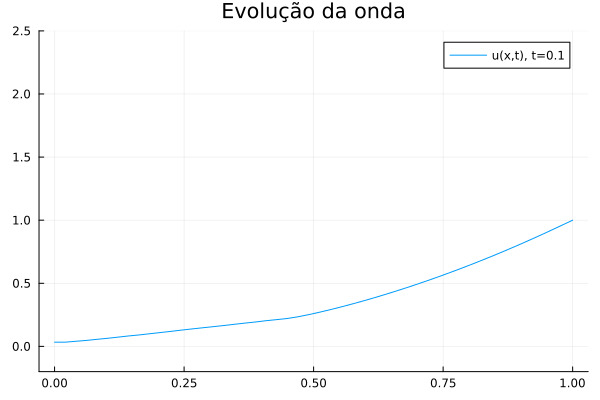
\includegraphics{Trabalho_final_AN_files/gifs/onda13-1}} &
        \adjustbox{max width=\dimexpr\textwidth/3\relax, max height=\dimexpr\textheight/5\relax}{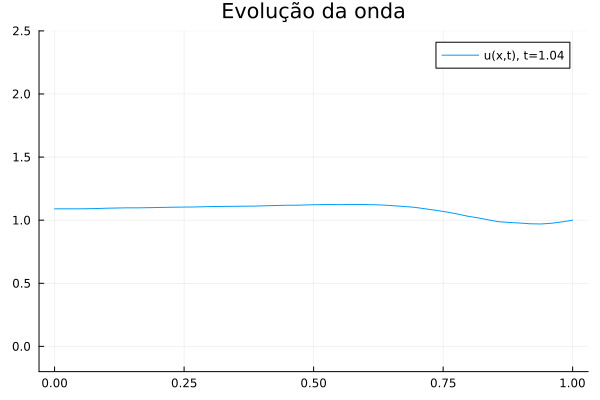
\includegraphics{Trabalho_final_AN_files/gifs/onda13-10}} &
        \adjustbox{max width=\dimexpr\textwidth/3\relax, max height=\dimexpr\textheight/5\relax}{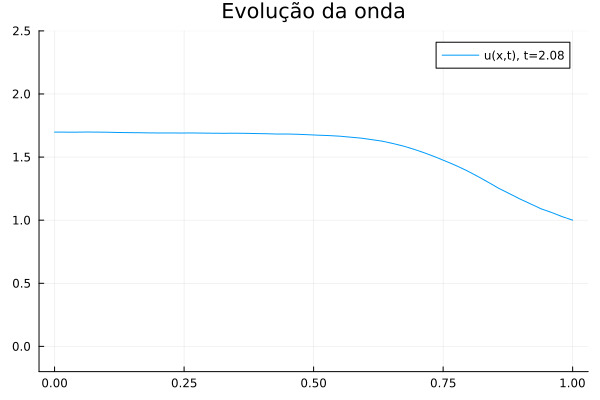
\includegraphics{Trabalho_final_AN_files/gifs/onda13-20}} \\

        % --- Linha 2 ---
        \adjustbox{max width=\dimexpr\textwidth/3\relax, max height=\dimexpr\textheight/5\relax}{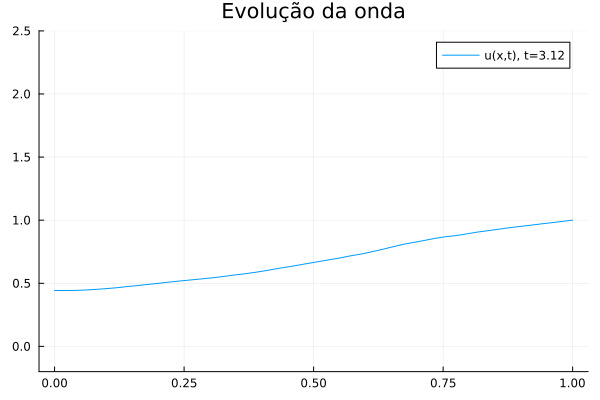
\includegraphics{Trabalho_final_AN_files/gifs/onda13-30}} &
        \adjustbox{max width=\dimexpr\textwidth/3\relax, max height=\dimexpr\textheight/5\relax}{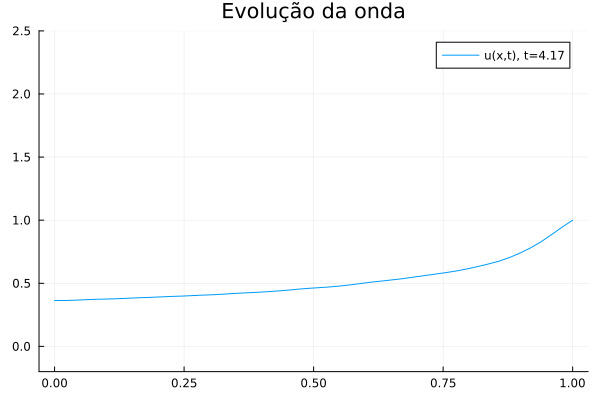
\includegraphics{Trabalho_final_AN_files/gifs/onda13-40}} &
        \adjustbox{max width=\dimexpr\textwidth/3\relax, max height=\dimexpr\textheight/5\relax}{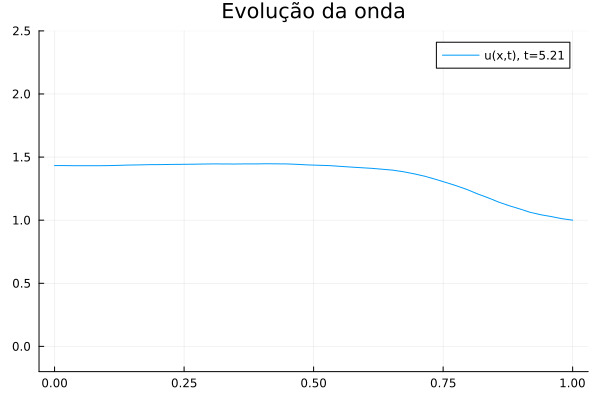
\includegraphics{Trabalho_final_AN_files/gifs/onda13-50}} \\

        % --- Linha 3 ---
        \adjustbox{max width=\dimexpr\textwidth/3\relax, max height=\dimexpr\textheight/5\relax}{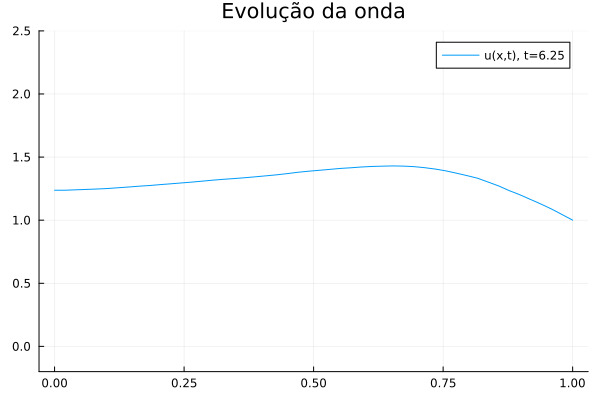
\includegraphics{Trabalho_final_AN_files/gifs/onda13-60}} &
        \adjustbox{max width=\dimexpr\textwidth/3\relax, max height=\dimexpr\textheight/5\relax}{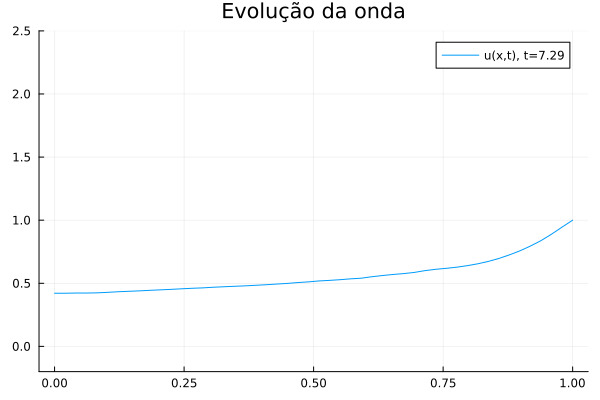
\includegraphics{Trabalho_final_AN_files/gifs/onda13-70}} &
        \adjustbox{max width=\dimexpr\textwidth/3\relax, max height=\dimexpr\textheight/5\relax}{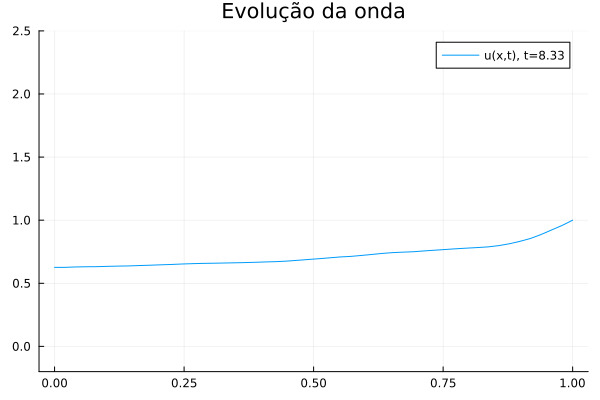
\includegraphics{Trabalho_final_AN_files/gifs/onda13-80}} \\
        
        % --- Linha 4 ---
        \adjustbox{max width=\dimexpr\textwidth/3\relax, max height=\dimexpr\textheight/5\relax}{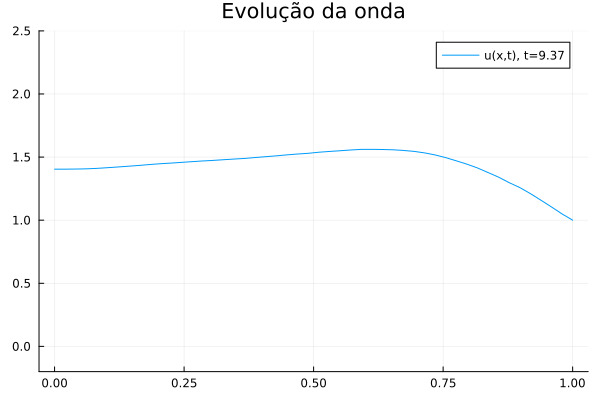
\includegraphics{Trabalho_final_AN_files/gifs/onda13-90}} &
        \adjustbox{max width=\dimexpr\textwidth/3\relax, max height=\dimexpr\textheight/5\relax}{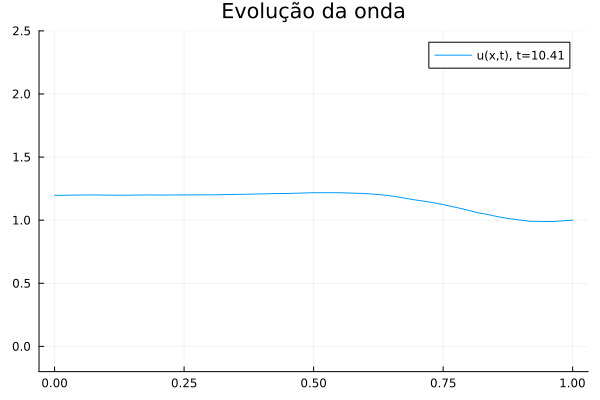
\includegraphics{Trabalho_final_AN_files/gifs/onda13-100}} &
        \adjustbox{max width=\dimexpr\textwidth/3\relax, max height=\dimexpr\textheight/5\relax}{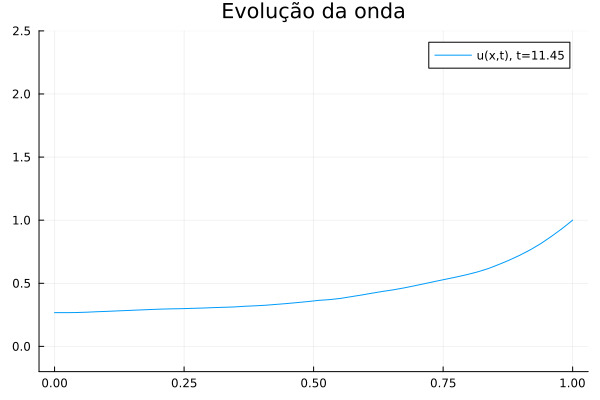
\includegraphics{Trabalho_final_AN_files/gifs/onda13-110}} \\

        % --- Linha 5 ---
        \adjustbox{max width=\dimexpr\textwidth/3\relax, max height=\dimexpr\textheight/5\relax}{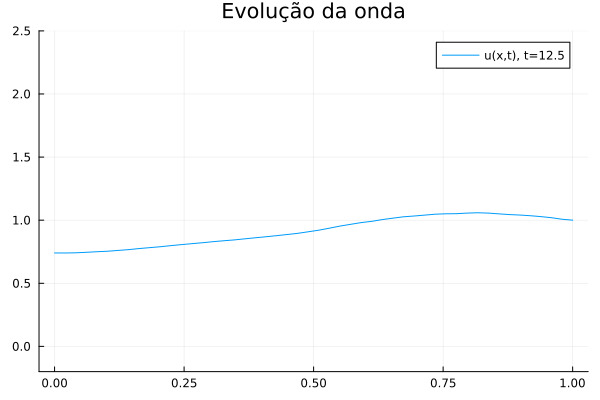
\includegraphics{Trabalho_final_AN_files/gifs/onda13-120}} &
        \adjustbox{max width=\dimexpr\textwidth/3\relax, max height=\dimexpr\textheight/5\relax}{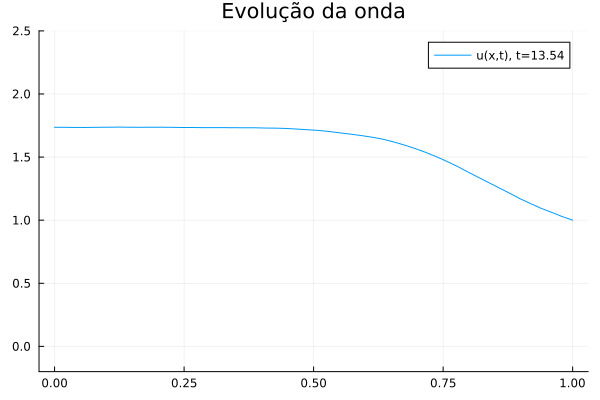
\includegraphics{Trabalho_final_AN_files/gifs/onda13-130}} &
        \adjustbox{max width=\dimexpr\textwidth/3\relax, max height=\dimexpr\textheight/5\relax}{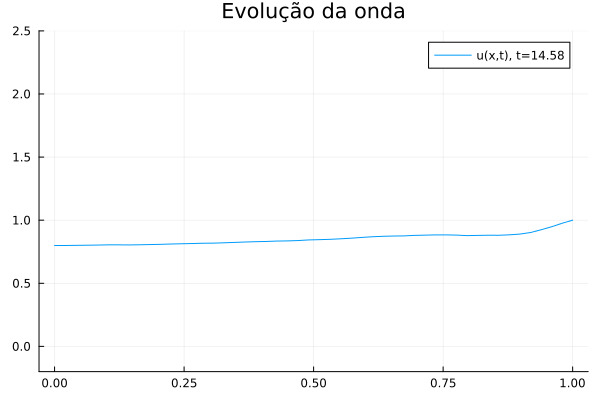
\includegraphics{Trabalho_final_AN_files/gifs/onda13-140}} \\
        
        % Se precisar de 15 imagens, você teria que usar 5 ondas (n=1 a 5) e os 15 frames
        % Os frames seriam: 0, 15, 30, 45, 60, 75, 90, 105, 120, 135, 150, 165, 180, 195, 210, 225

        % Para ter *exatamente* 15 imagens (5x3), precisamos de 15 frames.
        % Os frames solicitados são 0, 15, ..., 225 (16 frames). 
        % Adaptei para 15 frames: 0, 15, ..., 210, utilizando as primeiras 5 ondas. 
        % Para incluir o frame 225, você precisaria de um grid 6x3 ou 5x4.
        
        % Se quiser usar o frame 225, basta adicionar mais uma linha ao \begin{tabular}:
        % --- Linha 6 (Opcional - se o grid fosse 6x3) ---
        % \adjustbox{max width=\dimexpr\textwidth/3\relax, max height=\dimexpr\textheight/5\relax}{\includegraphics{Trabalho_final_AN_files/gifs/onda6-225}} & & \\
        
    \end{tabular}
\end{center}
        
    \hypertarget{conclusuxf5es}{%
\subsection{Conclusões}}

    Dentre os problemas apresentados, os mais difíceis são os que não tem
domínio limitado, tornando difícil a implementação para os pontos
extremos.

Outra parte complicada para os métodos numéricos é lidar com
descontinuidades.

A parte difícil das equações de advecção são principalmente a formação
de ondas de choque.


    % Add a bibliography block to the postdoc
    
    
    
\end{document}
